%% Local Variables:
%%% mode: latex
%%% TeX-master: t
%%% End:

% 通过使用draftformat或finalformat来控制是否有页眉,通过使用blackred或redhead来调整页眉格式
\documentclass[draftformat,redhead]{HUSTthesis}

% 所有其它可能用到的包都统一放到这里了,可以根据自己的实际添加或者删除。这样做
% 主要是为了避免class文件过于臃肿。
\usepackage{HUSTtils}

%\includeonly{body/chap02}
% \setcitestyle{authoryear, open={(},close={)}}

\usepackage[stable]{footmisc}

\usepackage{soul}


\newcommand*\red[1]{\textcolor{red}{#1}}
% \setul{0.5ex}{0.3ex}
\usepackage{xeCJKfntef}
\newcommand\redline[1]{\CJKunderline[skip=false,format=\color{red}]{#1}}

\usepackage{mathtools}

\DeclareMathOperator*{\argmax}{argmax}
\DeclareMathOperator*{\argmin}{argmin}
\DeclareMathOperator{\trans}{{\mathrm{T}}}
\DeclareMathOperator*{\avg}{Avg}
\newcommand*\abs[1]{\left \lvert#1 \right \rvert}
\newcommand*\norm[1]{\left \lVert #1 \right \rVert}
\newcommand\x{\bm{x}}
\newcommand\y{\bm{y}}
\newcommand\e{\bm{e}}
\newcommand\h{\bm{h}}
\newcommand\w{\bm{w}}
\newcommand\g{\bm{g}}
\newcommand\m{\bm{m}}
\newcommand\bs{\bm{s}}
\newcommand\bp{\bm{p}}
\newcommand\brho{\bm{\rho}}
\newcommand\bv{\bm{v}}
\newcommand\bu{\bm{u}}
\newcommand\mathr{\mathbb{R}}
\newcommand\mathd{\mathbb{D}}

% \usepackage[e]{esvect}
% \newcommand{\uv}[2][2mu]{\vec{#2\mkern-#1}\mkern#1}

% *** SPECIALIZED LIST PACKAGES ***
\usepackage{algorithm, algorithmic}
% \newcommand{\algorithmautorefname}{Algorithm}

\usepackage{breqn}

\usepackage{pifont}
\newcommand{\cmark}{\ding{51}}
\newcommand{\xmark}{\ding{55}}
\newcommand{\rfist}{\ding{192}~}
\newcommand{\rsecond}{\ding{193}~}
\newcommand{\rthird}{\ding{194}~}

\usepackage{marginnote}
\usepackage{multirow,makecell}
\usepackage{tabularx}
% \usepackage{ltablex} %load to using long tabularx
% \keepXColumns %solve the problem that tabularx does not fill full textwidth when using ltablex
\newcolumntype{Y}{>{\centering\arraybackslash}X}
\newcolumntype{P}[1]{>{\centering\arraybackslash}p{#1}}

\newcommand\ph{$\phantom{1}$} 
\newcommand\s{$^\star$}

\newlength{\twosubht}
\newsavebox{\twosubbox}

% 修改autoref前后间距,解决标签应用后的前后间距问题
\usepackage{letltxmacro}
\LetLtxMacro\oldautoref\autoref
\DeclareRobustCommand{\autoref}[1]{{\let\nobreakspace\space\oldautoref{#1}\space}}

\newcommand*\secref[1]{\ref{#1}节}

\usepackage{cleveref}
\newcommand{\crefrangeconjunction}{~--~}
\Crefname{table}{表}{表}
\Crefname{figure}{图}{图}

% %%  using line number.
% \usepackage[pagewise]{lineno}
% \makeatletter
% \def\makeLineNumberLeft{%
%   \linenumberfont\llap{\hb@xt@\linenumberwidth{\LineNumber\hss}\hskip\linenumbersep}% left line number
%   \hskip\columnwidth% skip over column of text
%   \rlap{\hskip\linenumbersep\hb@xt@\linenumberwidth{\hss\LineNumber}}\hss}% right line number
% \leftlinenumbers% Re-issue [left] option
% \makeatother




\begin{document}
%定义所有的eps文件在 figures 子目录下
\graphicspath{{figures/}}

% 生成封面,版权页,摘要

\frontmatter

%%% Local Variables:
%%% mode: latex
%%% TeX-master: t
%%% End:

\ctitle{基于随机映射的时间序列深度学习预测建模技术}

\xuehao{D201880***} 
% \xuehao{D201880970} 
\schoolcode{10487}
\miji{\hei\textbf{公开}}
\csubjectname{管理科学与工程} 
\cauthorname{张心泽}
\csupervisoronename{{鲍玉昆}}
\csupervisoronetitle{教\hspace{1em}授}
% 若存在第二指导老师,请取消下列注释。取消后,将自动显示第二导师。
% \csupervisortwoname{{李\hspace{1em}四}}
% \csupervisortwotitle{副教授}
\defencedate{2023~年~4~月~26~日} \grantdate{}
\chair{}%
\firstreviewer{} \secondreviewer{} \thirdreviewer{}


\etitle{Stochastic Deep Learning Based Time Series
Forecasting Techniques}
\edegree{Doctor of Philosophy in
    Management}
\esubject{Management Science and Engineering}
\eauthor{Zhang Xinze}
\esupervisorone{Prof. Bao Yukun}
% 若存在第二指导老师,请取消下列注释。取消后,将自动显示第二导师。
% \esupervisortwo{Assoc. Prof. Li Si}
\edate{April, 2023}

\dctab{\begin{tabular}{|P{0.9cm}|P{1.8cm}|P{1.8cm}|P{5.4cm}|}
    \hline
    &{\hei\textbf{姓名}}&{ \hei\textbf{职称}}&{\hei \textbf{单位}}\\
    \hline
    主席&X\hspace{1em}X&教授&武汉大学~信息管理学院\\
    \hline
    \multirow{4}{*}{委员}&X\hspace{1em}X&教授&武汉大学~信息管理学院\\
    \cline{2-4}
    &XXX&教授&华中科技大学~管理学院\\
    \cline{2-4}
    &XXX&教授&华中科技大学~管理学院\\
    \cline{2-4}
    &X\hspace{1em}X&教授&华中科技大学~管理学院\\
    \hline
\end{tabular}
}


%定义中英文摘要和关键字
\cabstract{
    时间序列预测建模技术是能源、金融和公共卫生等众多应用领域的重要技术。针对时间序列预测建模问题,深度学习预测建模技术因其优异的预测性能成为了近年的研究热点。然而,以卷积神经网络和循环神经网络为代表的深度神经网络预测模型受限于梯度下降权重训练方法,需要在反复训练权重参数的基础上才可具备优异的预测性能,因此带来昂贵的计算消耗;加之深度学习预测模型复杂的结构参数设置,使得深度学习预测建模技术面临建模效率低与模型选择难等问题。随机映射方法作为神经网络模型的一种非迭代训练方法,通过固定模型随机初始化的输入层与隐藏层权重,利用简单直接的闭式求解算法计算模型输出层权重,以此完成权重参数训练过程,因而可有效提升神经网络模型的构造效率。

    本学位论文基于随机映射方法对时间序列深度学习预测建模技术展开研究,针对随机深度神经网络预测模型在卷积结构和循环结构上的模型选择特有个性问题,提出随机卷积隐藏结构的构造优化方法和随机循环输出结构的构造优化方法;在此基础上探索随机深度神经网络特定代表结构的共性优化问题,提出随机深度神经网络预测模型一般结构下的二重特征选择方法和混合结构下的生长优化方法,进一步提升模型预测性能;在技术方法研究的同时,结合流感阳率预测、原油价格预测、电力负荷预测与电力价格预测等重要应用场景进行应用研究。本文的主要研究工作和创新性成果如下:


    首先,针对卷积结构的随机深度神经网络预测模型构造与优化问题,提出基于误差反馈随机建模和贪心优化的新颖构造与优化方法,解决了既有方法的参数选择不足及输出权重病态矩阵难题。通过向隐藏层中递归添加随机卷积核,利用最小二乘法局部更新输出权重,构造出随机卷积隐藏结构,并证明了该构造方法的收敛性;借助贪心搜索优化卷积核参数,使其在单卷积层内自适应选择不同宽度的卷积核,具备了不同尺度局部特征的学习能力。在合成数据和多项现实数据上的实验表明,该模型具有极高的模型构造与选择效率,表现出与梯度下降训练的深度学习预测模型媲美甚至更优的预测性能。

    其次,针对循环结构的随机深度神经网络预测模型构造与优化问题,提出了基于状态遮掩和粒子群优化的新颖构造与优化方法,解决了既有方法忽视的输出结构优化问题。基于对循环神经网络输出结构的随机映射实现,分析得出不同输出结构的异同优劣;通过向循环隐藏特征表示施加状态掩码,提出状态遮掩的随机循环输出结构,借助粒子群优化自适应选择循环隐藏特征表示和目标的映射取舍,提升了输出结构的学习能力。在人工合成、电力负荷和室外温度数据集上的实验表明,与既有随机循环神经网络及其输出结构优化方法相比,基于所提方法构造的模型具备明显的多步预测优势。

    再次,针对一般结构的随机深度神经网络预测模型特征选择问题,提出了基于二重特征结构选择和树状结构帕森斯估计的新颖特征选择方法,消除了既有选择方法的一维输入特征结构局限。结合深度神经网络的时步多维度读取能力,利用滑动窗口构造时步多维度的二维输入特征结构;通过向每一输入时步添加时步掩码,建立基于时步维度与时步掩码组合的二重特征结构表示,借助树状结构帕森斯估计自适应优化特征结构参数,降低了抽象特征的学习难度。在人工合成、电力负荷和电力价格数据集上的实验表明,与既有卷积与循环结构随机深度神经网络及其特征选择方法相比,基于所提方法优化的模型具有更好的预测准确性与稳定性。

    最后,针对混合结构的随机深度神经网络预测模型构造与优化问题,提出了基于误差反馈生长和三阶段优化的新颖混合结构构造与优化方法,消除了既有方法的单一结构局限。通过递归添加不同结构的随机子网络,利用岭回归局部更新输出权重,构造出鲁棒的混合隐藏结构,并证明了该构造方法的收敛性;通过预优化、子训练和调正则的三阶段优化方法对迭代添加的子网络进行完整优化,使其自适应选择出多种结构的子网络及参数,融合了不同深度结构的学习能力。在人工合成、空气污染和电力负荷数据集上的实验表明,与多种既有随机深度神经网络模型相比,基于所提方法构造的模型具有更好的预测性能。
}

\ckeywords{时间序列预测;深度学习;随机映射;卷积神经网络;回声状态网络}

\eabstract{
    Time series forecasting is of great importance for a learning system in dynamic environments, playing a vital role in many real-world applications, such as energy, traffic, finance, and industry. Recent studies have shown that deep learning technique has shown intriguing prediction performance, leading to extensive research on the applications of the DNN models for time series forecasting. However, represented by the convolutional neural network and recurrent neural network models, the deep neural network--based forecasting models have complex architecture-related parameters and rely on gradient-based algorithms to train the weight-related parameters, making it extremely time-consuming and challenging to well establish a forecasting model. As an alternative method of training the neural network model, the stochastic mechanism fixes the weights of the input layer and the hidden layer after random initialization, and uses a simple and direct closed-form solution algorithm to calculate the weight of the output layer of the model, which can effectively improve the construction efficiency of the neural network model. 
    
    Therefore, this study investigates time series deep learning prediction modeling technology based on the stochastic mechanism, pays attention to the structure selection problems under the specific structures, and proposes the hidden structure construction method of the stochastic convolutional neural network and the output structure selection method of the stochastic recurrent neural network. On this basis, the optimization problems under the universal structure are explored, and the feature selection method as well as the parameter optimization method of the stochastic deep neural network prediction model are proposed to further improve the prediction performance of the models. At the same time, the application research is carried out in combination with important application scenarios, such as influenza prediction, crude oil price prediction, electricity load prediction, electricity price prediction, and so on. The main contributions of this dissertation are summarized as follows:
    
    Focusing on the model construction problem of stochastic convolutional neural network--based forecasting model, a novel error-feedback stochastic modeling strategy and greedy-based selection algorithm are proposed to craft the random convolutional neural network for time series forecasting. The proposed method suggests that random filters and neurons of the error-feedback fully connected layer are incrementally added to steadily compensate for the prediction error during the construction process, and then a greedy-based filter selection is introduced to enable the model to extract the different sizes of temporal features. Comprehensive experiments on the simulated dataset and several real-world datasets show that the proposed method exhibits stronger predictive power and lower computing overhead compared to trained state-of-the-art deep neural network models.

    Focusing on the model construction problem of stochastic recurrent neural network--based forecasting model, a novel state mask strategy with particle swarm optimization is proposed to construct the random recurrent output structure for time series forecasting. Based on the investigation of the stochastic implementation of different recurrent output structures of training-based recurrent neural networks, the proposed method adds a mask to each step of the recurrent hidden features, and then a particle swarm optimization based mask selection is introduced to evolve the mapping relationships from recurrent hidden features to their targets, which improves the learning ability of the stochastic recurrent output architecture. Compared with the stochastic recurrent neural networks with the existing output architecture selection method, comprehensive experiments on the simulated dataset, electricity load dataset, and outside temperature dataset demonstrate the superiority of the proposed method. 

    Focusing on the input feature selection problem of stochastic deep neural network--based forecasting model, a novel dual feature-structured selection method with tree-structured parzen estimator is proposed. Based on the ability of deep neural architecture that can model multiple dimensions in each input time step, a multiple-step-dimension two-dimensional feature structure is established with a moving window schema. The proposed method adds a mask to each input step to represent the two-dimensional feature structure with the combination of step dimension and step mask, and then tree-structured parzen estimator is introduced to evolve the feature structure, which improves the learning ability of the stochastic deep neural networks. Compared with the stochastic deep neural networks with the existing feature selection method, comprehensive experiments on the simulated dataset, electricity load dataset, and electricity price dataset demonstrate the superiority of the proposed method.

    Focusing on the model construction problem of stochastic deep neural network--based forecasting model, a novel error-feedback triple-phase optimization strategy is proposed to grow stochastic deep neural network--based predictor with mixed deep neural architectures. The proposed method incrementally adds diverse deep subnetworks to the network, where the output weights of the subnetworks are calculated via ridge regression to improve the robustness of the constructed model, and the parameters of the subnetworks are evolved with pre-tuning, sub-tuning, and reg-tuning optimization, making the network take advantage of different deep neural architectures. Compared with the existing stochastic deep neural networks, comprehensive experiments on the simulated dataset, air pollution datasets and electricity load datasets demonstrate the superiority of the proposed method.
}

\ekeywords{
    Time series forecasting; deep learning; stochastic mechanism; convolutional neural network; echo state network
}

\makecover

%目录
\tableofcontents

% 对照表
% \include{body/denotation}

\mainmatter

\raggedbottom
%% using line count
% \linenumbers

% \nolinenumbers
%%% 结论
%%% mode: latex
%%% TeX-master: t
%%% End:

\chapter{绪论}
\section{研究背景与意义}
预测问题是经济生活、工业生产、公共卫生和能源系统等众多应用领域的重要问题。若能基于观测的现实预测出未来将要发生的现象,则能为控制或决策提供参考。自然,科学准确的预测是正确决策的重要依据。
然而,现实数据往往是复杂且动态的,难以通过某一确定性的物理定律或因果关系精确推算出未来的状态。因此需要考虑依赖于时间的现象,基于数据自身的历史观测值,建立预测模型从而估计和推测出未来状态,这样处理预测问题的方式被称为时间序列预测。其中,根据数据发生的历史时间顺序所得到的序列观测值即是时间序列数据。
在现实背景下,时间序列数据常常呈现出规模庞大、模态多样和关联复杂等性质,表现出感知度量难、特征融合难和模式挖掘难等问题。
对于这种动态机制不确定的数据,如何建立一种建模技术来解决大规模时间序列数据非平稳状态下的动态性预测问题,对学界和业界都具有重要的理论价值和实际意义。

% \section{研究意义}
在预测科学的发展进程中,各种预测技术和方法推陈出新。
其中,以卷积神经网络(Convolutional neural network,CNN)和循环神经网络(Recurrent neural network,RNN)为代表的深度学习(Deep learning,DL)预测建模技术成为该领域近年来的研究热点。深度学习是一种大数据背景下基于深度神经网络(Deep neural network,DNN)的机器学习(Machine learning,ML)建模思想,着重研究样本数据的内在规律与表示层次~\cite{hintonReducing2006}。相较于传统的统计机器学习方法,即基于统计模型依赖经验选取特征的浅层学习方法,如支持向量机(Support vector machine,SVM)和多层感知机(Multilayer perceptron,MLP)等,DNN采用卷积池化或循环记忆的网络结构,在成功解决了复杂网络结构下训练初始化~\cite{heDelving2015,glorotUnderstanding2010}与梯度不稳定问题~\cite{mikolovContext2012,pascanuDifficulty2013}后,构造的模型具有优异的特征学习能力和预测性能,并根据网络结构的不同,在面对海量时间序列数据时表现出不同的效率与性能侧重优势。

例如,基于卷积结构的DNN(即CNN)预测模型通过卷积与池化,在降低网络参数的同时进行局部特征的抽象表征,使得模型具备良好的学习能力与效率优势;而基于循环结构的DNN(即RNN)预测模型考虑输入数据的时序关系,通过历史的隐藏特征表示与当前的输入数据特征,迭代完成样本的时序特征抽象学习,使得模型具备优异的预测性能。因此,近年来涌现出大量基于深度学习建模技术的预测应用研究,这些技术方法在多项应用领域,如金融市场~\cite{wuImproved2019,zhaoDeep2017,sezerFinancial2020},能源市场~\cite{caiDayahead2019,lindbergLongterm2019,shiDeep2018}和交通管理~\cite{laptevTimeseries2017,wangTraffic2016,xiaoShortterm2019}等,取得了显著的预测效果,表现出良好的应用前景。

尽管深度学习预测建模技术在管理领域中得到不断推广与应用,但研究表明,深度学习模型与浅层学习模型一样受到多种技术因素的影响(如神经网络结构,输入选择和输出策略等)~\cite{sezerFinancial2020,lindbergLongterm2019}。在现实的时间序列预测任务中,这些在其他领域(如图像识别、目标检测、文本分类和机器翻译等)展现出优异性能的深度学习算法会因不恰当的模型参数设置而无法表现出预期性能。此外,深度学习模型普遍依赖梯度下降(Gradient decent,GD)方法~\cite{sutskeverImportance2013,kingmaAdam2015,reddiConvergence2018,allen-zhuConvergence2019,loshchilovDecoupled2019}多次迭代训练其权重参数以优化其预测性能。同时,现有的深度学习预测建模技术普遍依赖人工经验来解决模型神经网络结构设计、参数设置和特征选择等模型选择问题,使得研究人员与从业人员不得不付出高昂的计算开销来摸索与尝试合适的模型参数与输入特征,降低了深度学习建模技术在时间序列预测问题中的应用效率与实际性能。因此,高效解决深度学习预测建模技术中的模型选择问题,以探索和提高其在现实典型时间序列情景中的预测性能和学习效率,是发展时间序列深度学习预测模型及其应用研究中的重要内容。

与梯度下降方法的迭代学习机制不同,随机映射是一种采用非迭代学习机制的神经网络建模方法~\cite{scardapaneRandomness2017,liInsights2017,wang2015jiyu,shen2018jiyu}。随机映射方法通过随机初始化并固定神经网络输入层权重与隐藏层权重,结合闭式求解算法确定输出层权重,构造出随机(Stochastic)神经网络模型。与梯度下降方法构造的训练(Trained)神经网络模型相比,随机神经网络模型具有极低的计算开销、优异的学习效率与良好的非线性表达能力。基于随机映射方法,已发展出极限学习机(Extreme learning machine,ELM)~\cite{shen2017jiyu}、随机向量函数链接网络(Random vector version of the functional-link,RVFL)~\cite{fu2021jiyu}等神经网络学习技术,并在时间序列预测任务中得到了广泛应用~\cite{scardapaneRandomness2017,caoReview2018,tanakaRecent2019}。

然而,基于随机映射的深度神经网络,即随机深度神经网络(Stochastic deep neural network,SDNN),其预测建模技术研究却较未深入。一方面,既有方法多聚焦于随机映射方法的直接应用~\cite{yuImpact2019,huForecasting2020,sunReview2020,hu2021jiyu}或是对现有SDNN模型的组合集成~\cite{wang2018effective,lv2018stacked,lv2019jiyu};另一方面,随机映射方法在大幅提升建模效率的同时,使得所构造的SDNN模型的预测性能对网络结构与参数设置更加敏感,且由于与梯度下降方法在神经网络模型权重参数确定机制上的本质差异,使得传统神经网络建模技术下的模型选择方法对于SDNN预测模型而言适用有限。

此外,SDNN预测模型的模型选择对象及问题,在以卷积和循环为代表的不同特定神经网络结构实现方法下,呈现出个性且复杂的特点。
例如,基于卷积结构的SDNN预测模型在进行模型选择时,区别于传统的训练CNN模型,在卷积结构SDNN模型由多个卷积核组成的随机卷积层中,每个随机卷积核的结构及权重分布都可以是不同的~\cite{zhangErrorfeedback2021};再如,基于循环结构的SDNN预测模型在进行学习建模时,每个循环节点都可生成当前输入的对应目标输出值,区别于传统的训练RNN模型,随机映射方法下其输出权重的闭式求解需考量这些节点的选取与否。
这些特性问题使得基于SDNN的预测建模技术需要考虑不同神经网络结构实现下的方式特点,建立针对且有效的模型选择方法,以更好提升SDNN模型预测效能。

同时,SDNN建模技术在不同结构实现下的特定优化问题外,亦存在区别于传统机器学习方法与随机浅层神经网络模型的共性优化问题。例如,卷积层的单卷积核多通道输入能力\cite{wangTraffic2016}和循环层的单循环节点多时步输入能力\cite{bandaraForecasting2020}均可将单变量时间序列预测建模中的传统一维输入结构提升为二维输入结构,使得时间序列数据在SDNN预测模型中的特征选择这一关键问题更为复杂。


通过对以上背景的分析可知,有必要进行系统、全面、针对且深入的SDNN预测建模技术研究。基于此,本研究在充分利用DNN拓扑结构优异的特征学习能力和随机映射方法低开销与高效率的建模优势基础上,关注SDNN预测建模技术模型选择的问题与挑战,研究SDNN预测模型构造与优化的创新方法与提升策略。

首先,针对SDNN预测模型在不同典型代表结构下实现下的特定问题,例如SDNN预测模型在基于卷积结构实现时的隐藏结构构造与优化问题以及基于循环结构实现时的输出结构构造与优化问题,分别进行深入且细致地探索,创新提出高效且自适应的随机映射卷积隐藏结构构造方法和循环输出结构优化方法;而后,归纳SDNN预测模型在不同结构实现时的共性优化问题,例如特征选择问题,提出一般结构下的SDNN新型时间序列输入特征选择方法;最后,结合不同深度神经网络结构的特有能力优势,例如卷积结构的局部特征学习能力和循环结构的长期特征学习能力,以及考虑SDNN预测建模的整体优化问题,提出混合结构的SDNN预测模型生长与优化方法,构造出强健、鲁棒且准确的SDNN预测建模技术框架。

本研究旨在建立基于随机映射的深度学习预测建模方法,通过结合随机映射方法的建模效率优势与DNN模型的预测性能优势,聚焦既有SDNN预测模型方法的关键问题与挑战,创新提出一系列SDNN预测模型构造与优化方法,并用于解决管理应用中多种复杂现实时间序列预测问题,以期为决策提供更为高效且智能的支持。

在理论层面,本论文将深入研究不同神经网络结构下的SDNN预测模型和新的理论分析框架,如构建基于卷积结构和混合结构的SDNN预测模型的预测误差收敛性分析框架,直观理解SDNN预测模型的构造与决策逻辑。这些新颖的模型与理论分析框架的提出有助于丰富既有SDNN预测建模技术研究的理论体系,具有一定的理论意义。
% ,为完善DNN预测模型的解释性研究提供一定支撑。

在方法层面,本论文将构造多套预测模型构造与优化方法,包括适用于卷积结构、循环结构、一般结构至混合结构SDNN模型的优化技术,形成从特定到一般再到混合的综合技术体系与框架,为SDNN预测建模技术的复杂模型选择问题提供新颖的方法与思路。这些新方法的提出将拓展既有SDNN预测建模技术研究的方法体系,为完善SDNN预测模型的模型选择问题研究提供一定支撑。

在现实层面,本论文将立足于现实时间序列预测任务的多个场景,包括公共卫生领域中的流感阳性样本率预测任务、能源市场中的原油价格预测任务、金融市场中的股票指数预测任务、大气污染中的PM2.5预测任务、电力系统中的电力负荷与电力价格预测任务等。基于模型在不同场景下的预测结果和优势特点,如基于卷积结构SDNN模型的效率优势和基于混合结构SDNN模型的性能优势,可为管理部门制定决策提供效能层面的不同支撑,对SDNN预测建模技术的应用具有良好的现实意义。

\section{研究面临的关键问题}

针对时间序列预测建模这一重要问题,基于SDNN的预测建模技术因其高效的构造效率和良好的预测潜能受到了广泛关注和应用,但既有方法面临着如下关键问题:

(1)如何构建基于卷积结构SDNN预测模型的新颖构造及自适应优化方法,以解决已有卷积结构SDNN预测建模技术中参数选择时的人工依赖、输出权重求解时的病态矩阵和预测过程的不稳定性,是本研究的关键问题。

SDNN模型预测性能对于隐藏结构的设计与参数设置以及输出权重的闭式求解方式非常敏感,这一现象在卷积结构的实现中尤为明显。原因在于,SDNN建模方法下接隐藏层的输入权重与隐藏权重是随机且固定的,输出层权重是基于隐藏特征表征和预测目标的映射通过闭式求解予以确定。更具体的,一方面在卷积结构的SDNN模型实现中,输入层与隐藏层权重统一地被卷积层权重所取代,同时卷积核权重的随机设置与其结构参数息息相关,使得卷积结构SDNN预测模型性能敏感于卷积层结构参数及随机权重,然而既有SDNN的卷积实现方法在进行隐藏卷积结构构造时依赖于人工试错,缺少自适应确定隐藏结构及参数设置的构造与选择方法;另一方面,同时,随着卷积核数量的增加会导致输出层读取的隐藏特征维度呈倍数增大,使得既有的输出层权重求解方法出现病态矩阵问题(Ill-posed problem),从而降低了输出层权重的求解质量,严重影响了模型的拟合能力和预测稳定性。因此,有必要设计一种能够自适应确定隐藏卷积结构及参数,兼具良好预测性能和高效建模效率的SDNN卷积结构实现方法,以更好发挥卷积结构的建模效率优势。

% 通常而言,SDNN模型对时间序列数据的表征通过隐藏层结构的随机映射和输出层的特征学习共同完成。随机映射方法下链接隐藏层的输入权重与隐藏权重是随机且固定的,输出层权重是基于隐藏特征表征和预测目标的映射通过闭式求解予以确定,因此。既有SDNN的卷积实现方法在进行隐藏卷积结构构造时依赖于人工试错,缺少自适应确定隐藏结构及参数设置的构造与选择方法;同时,随着卷积核数量的增加会导致输出层读取的隐藏特征维度呈倍数增大,使得既有的输出层权重求解方法出现病态矩阵问题,从而降低了输出层权重的求解质量,严重影响了模型的拟合能力和预测稳定性。因此,有必要设计一种能够自适应确定隐藏卷积结构及参数,兼具良好预测性能和高效建模效率的SDNN卷积结构实现方法,以更好发挥卷积结构的建模效率优势。

(2)如何构建基于循环结构SDNN预测模型的新颖构造及自适应优化方法,以解决已有循环结构SDNN预测建模技术所忽视的循环隐藏特征表示与预测目标的复杂对应问题,是本研究的关键问题。

区别于直接对局部特征进行高效前馈表征的卷积结构,SDNN循环结构实现方法则更侧重于捕捉与学习时序性特征,利用循环构造当前时间序列观测值与目标值间的映射完成预测建模。在此过程中,每个循环节点都将生成当前读取输入值的对应隐藏特征表示,建立出隐藏特征表示与拟合目标的时间序列对应队列,基于队列内的隐藏特征表示与拟合目标的对应关系闭式求解输出权重。然而,由于时间序列数据的复杂性,队列内的匹配关系并不一定都有助于得到良好的输出权重解。在进行匹配选取时,既有方法采用直接丢弃初始区间的做法,忽视了时间序列隐藏特征表示与拟合目标匹配队列的复杂性,从而降低了输出层权重的求解质量,限制了SDNN循环结构实现方法的时序特征学习能力。因此,有必要设计一种能够自适应确定循环输出结构及参数,兼具良好预测性能和高效建模效率的SDNN循环结构实现方法,以更好发挥循环结构的预测性能潜力。

(3)如何将特征选择与深度神经网络结构相结合,以利用已有SDNN预测模型特征选择方法所忽视的时步多维度输入能力,提出适用于以卷积和循环结构为代表的一般结构SDNN预测模型的自适应特征选择方法,是本研究的关键问题。

与传统机器学习方法或浅层神经网络方法不同,以卷积结构和循环结构为代表的DNN因其隐藏结构的特殊性,如卷积层中的单卷积核多通道结构和循环层中的单循环节点多神经元输入结构,使得DNN预测模型能够将传统的单变量输入的一维特征结构表示在每个输入时步节点囊括入邻近的时域特征,从而将传统一维输入特征作为特例,呈现出复杂的二维输入特征结构表示。此外,相较梯度下降方法训练的DNN预测模型,随机映射方法内在随机机制在提升建模效率的同时,一定程度上降低了模型直接对时间序列原始输入特征进行抽象学习的能力,因此更需要从复杂的输入中挖掘与选择出合适的特征以提升模型预测性能。然而,既有的SDNN预测模型特征选择方法未考虑时间序列输入数据的二维结构性质,仍在一维输入结构表示上进行特征取舍,削弱了特征选择对于SDNN预测模型性能的提升能力。因此,有必要设计一种种能够自适应确定输入特征结构及取舍的SDNN预测模型特征选择方法,以进一步提高模型的预测精度。

(4)如何将不同深度神经网络相结合,以消除已有SDNN预测建模方法固守于某一特定结构的局限,提出可包纳卷积结构、循环结构及其他DNN结构的混合结构SDNN预测模型构造与自适应优化方法,是本研究的关键问题。

面对复杂不同的时间序列预测任务,基于单一结构主体的SDNN预测模型可能难以完全胜任。事实上,SDNN预测模型在不同的神经网络结构实现下侧重不同的特征学习能力,如卷积结构对局部特征的学习能力和循环结构对时序特征的学习能力。故需要混合不同深度神经网络结构,以融合不同结构的性能优势,使SDNN预测模型具备综合的学习能力。然而,既有的SDNN预测建模方法局限于单一结构实现。同时,混合结构的SDNN预测模型对模型参数的选择与建模稳定性提出了更高要求。因此,有必要设计一种可兼容不同种类深度神经网络结构,能够自适应确定隐藏结构组成类别及对应参数,稳健且鲁棒的混合结构SDNN预测模型构造与选择方法,以更好解决时间序列预测问题。

\section{研究内容与创新点}
本文研究目标如下:以精准和高效的时间序列预测为目标,基于随机映射方法与深度神经网络预测模型,构造自适应确定模型参数与特征,准确、高效且稳健的SDNN预测建模技术,以适应复杂不同的时间序列预测场景需要,为管理决策提供更为快捷、智能、安全和稳定的支持。为此,本研究探索SDNN预测建模技术既有方法的关键问题,创新提出对应解决方法和改进策略,利用主流人工时间序列数据和多种现实时间序列数据验证所提方法策略的有效性,以期具备一定的理论意义和良好的现实意义。

\subsection{研究内容}
本研究以高效准确时间序列预测为研究目的,以SDNN预测建模技术为主要研究方法,其主要研究内容如下:

(1)基于卷积结构的SDNN预测模型构造与优化方法

既有SDNN预测模型的卷积结构实现方法依赖于人工设计隐藏结构,其全局更新输出权重的方式易产生不稳定的预测结果,使得随机映射卷积结构的效率优势意义有限。基于此,提出一种基于误差反馈的SDNN预测模型卷积结构构造与优化方法,采用递归添加随机卷积核的方式,逐步构造隐藏结构,通过误差反馈机制局部更新输出权重以此稳步降低模型预测误差,使得所构造模型具有理论保证的收敛误差;同时,利用贪心算法解决卷积结构参数与随机权重选择问题以增强模型感知不同尺度局部特征的能力;最后,结合人工合成时间序列数据、比特币价格、流感阳性样本率、国际原油价格和股票指数时间序列数据,验证所提方法的准确性、收敛性和建模效率。

(2)基于循环结构的SDNN预测模型构造与优化方法

既有SDNN预测模型的循环结构实现方法在采用闭式求解算法计算输出权重时,一般采用直接丢弃循环队列初始区间内隐藏状态与目标间映射关系的方式,这种做法未考虑参与求解的隐藏特征表示与目标队列的复杂关系,限制了随机映射循环结构的预测建模潜能。基于此,考虑堆栈结构、线性解码器结构和循环解码器等不同循环输出结构的实现形式,提出一种基于状态遮掩的SDNN预测模型循环结构构造与优化方法,利用粒子群优化算法对隐藏特征表示与目标队列进行选择以增强模型感知复杂时序特征的能力。同时,结合人工合成时间序列数据、电力负荷和室外温度时间序列数据,从预测准确度和结果稳定性等方面验证所提方法的有效性。

(3)SDNN预测模型的二重特征结构选择方法

既有SDNN预测模型特征选择方法局限于一维的时步单输入结构,其直接对各时步输入特征进行选择的方式未考虑深度神经网络结构对输入时间序列数据的时步多维度结构表示能力,限制了SDNN预测模型的特征学习能力。基于此,提出一种基于输入特征结构变换的二重特征结构优化方法,对输入时间序列的输入步长、时步维度和输入时步加以优化,利用树状帕尔森估计算法优化“时步维度-时步掩码”的输入特征结构元组,完成模型的特征结构选择,进一步提升SDNN模型的时间序列数据学习能力与预测精度。同时,结合人工合成时间序列数据、电力负荷和电力价格时间序列数据,以及不同深度神经网络结构验证所提方法的有效性。

(4)SDNN预测模型的混合结构生长与优化方法

既有SDNN预测模型的构造与选择方法局限于单一的深度神经网络结构,而不同类别的神经网络结构侧重不同的时间序列特征学习能力,现有方法难以主动适应复杂不同的时间序列预测场景。基于此,提出一种基于混合结构的SDNN预测模型生长与优化方法,通过迭代添加不同种类随机深度子网络构造隐藏结构,引入正则项改进误差反馈生长策略以此确定子网络输出权重,建立预优化、子训练和调正则的三阶段优化策略对子网络参数及权重进行优化,以此提升模型的学习能力、预测精度和稳定性。同时,结合人工合成时间序列数据、空气污染和电力负荷时间序列数据,验证所提方法的有效性、必要性、稳定性和收敛性。


\subsection{研究创新点}
基于对面向时间序列预测问题的SDNN预测建模技术理论与应用研究,本文主要创新点如下:

1)针对卷积结构SDNN预测模型中卷积层参数选择及输出权重病态矩阵难题,通过构造误差反馈随机建模构造策略和建立贪心搜索选择方法,提出基于卷积结构的SDNN预测模型构造与优化方法。其创新之处包括以下方面:

(1)通过代数推导证明了基于该方法所构造的预测模型具有随着卷积核的增加而单调下降的预测误差,以此保证了所提方法的收敛性,且其确定的输出权重与既有方法相比具有更小的$L_2$范数,以此提升了模型的预测稳定性;

(2)区别于既有方法仅能用相同宽度的卷积核构造单卷积层,通过贪心选择由不同卷积核宽度组成的备选集,使得模型能够在迭代构造模型的过程中自适应确定卷积参数,其构造的单卷积层具备不同宽度的卷积核,使模型借助单卷积层具备不同尺度局部特征的学习能力;

(3)在人工合成数据、流感阳率数据、国际原油价格数据和股票指数数据上的实验表明,与梯度下降训练的深度神经网络预测模型相比,基于本方法所构造的模型在具备相近甚至更优的预测准确度同时具备极高的建模效率,验证了所提方法的有效性。


2)针对循环结构SDNN预测模型中循环隐藏特征表示与预测目标间的复杂关系处理难题,通过考虑多种SDNN循环输出结构实现方法和利用粒子群优化算法,提出基于循环结构的SDNN预测模型构造与优化方法。其创新之处包括以下方面:

(1)在既有随机映射循环输出结构实现方法外,借鉴梯度下降训练循环神经网络输出结构提出多种随机映射循环输出结构实现方法,并实验分析不同输出结构间的异同优劣,为随机映射循环输出结构的实现应用提供更多支撑;

(2)区别于既有现方法强制丢弃一定初始区间内所有的隐藏状态表示,通过对循环结构每个循环节点生成的隐藏状态表示及目标施加状态掩码,借助粒子群优化方法进行循环队列完整区间内的隐藏状态表示取舍,使得模型能够更好学习输入时间序列数据的时序性特征,降低模型输出权重的学习难度,提升模型的预测性能;

(3)在人工合成数据、电力负荷数据和室外温度数据上的实验表明,与已有的SDNN循环输出结构优化方法相比,所提方法具备更好的多步预测准确度和稳定性,验证了所提方法的有效性。


3)针对以卷积和循环结构为代表的一般SDNN预测模型多输入时步多时步维度特征选择难题,通过构造二维输入特征结构和利用树状帕尔森估计算法,提出了SDNN预测模型的二重特征结构选择方法。其创新之处包括以下方面:

(1)区别于既有SDNN特征选择方法局限于一维输入结构,且仅利用时步掩码对输入特征进行选择的方式,基于以卷积结构和循环结构为代表的深度神经网络时步多维度特征读取能力,利用滑动窗口构造出时步多维度的新颖输入特征结构,丰富模型输入信息;

(2)将既有的多输入特征选择方法作为被囊括的特例,通过树状帕尔森估计算法对输入的二维特征结构时步维度和时步掩码参数同时进行优化,使得模型能够根据不同的时间序列任务在每个时步输入节点丰富邻近特征信息的同时,去除冗余和嘈杂的输入时步节点,降低模型抽象特征的学习难度,提升模型的预测性能;

(3)在人工合成数据、电力负荷数据和电力价格数据上的实验表明,与已有的SDNN特征选择方法相比,基于所提方法构造的模型具有更优的预测性能,验证了所提方法的有效性。

4)针对混合卷积、循环和其他深度神经网络结构的SDNN预测模型构造与自适应优化难题,通过改进误差反馈生长策略和建立三阶段优化算法,提出了SDNN预测模型的混合结构生长与优化方法。其创新之处包括以下方面:

(1)区别于既有SDNN预测模型传统的单一隐藏神经网络结构,构造混合结构的生长策略,通过矩阵分析证明了基于该策略所构造的预测模型随着不同结构子网络的加入具有单调下降的预测误差,以此保证了所提方法的收敛性,且通过向输出权重的计算过程引入正则项,避免了既有随机映射方法更新输出权重时可能遇到的病态矩阵问题和过拟合问题,提升了模型的鲁棒性;

(2)区别于既有SDNN参数优化方法仅对部分参数进行选择的做法,提出预优化、子训练和调正则的三阶段优化方法对定义子网络的结构参数、输入与隐藏权重参数,以及输出权重进行完整优化,使得模型能够根据不同的时间序列任务自适应地生长神经网络结构与选择参数,进一步提升模型预测性能;

(3)在人工合成数据、空气污染数据和电力负荷数据上的实验表明,与已有的先进SDNN预测模型相比,基于所提方法构造的模型具有更优的预测性能,验证了所提方法的有效性。

% \clearpage
\begin{figure}[!t]
    \centering
    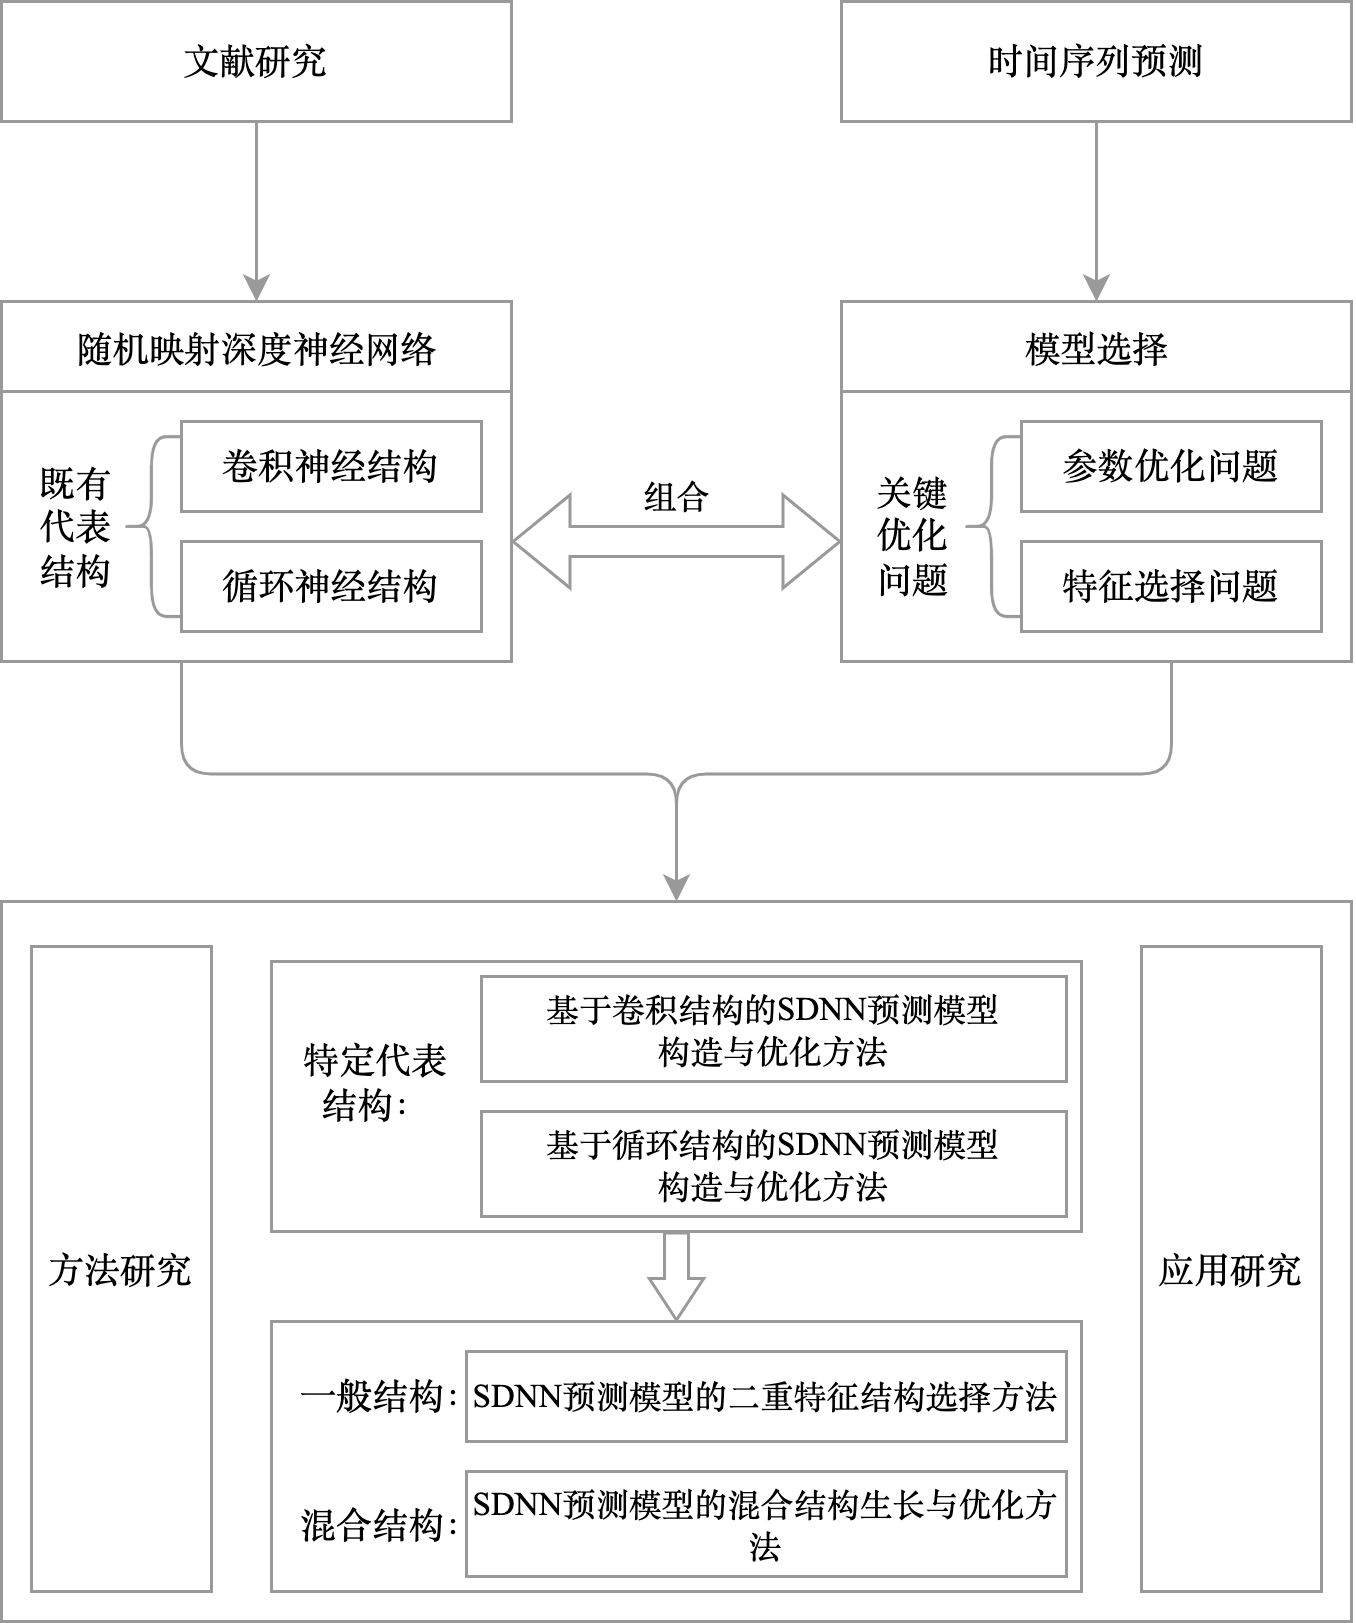
\includegraphics[width=0.8\linewidth]{float/ch.intro/thesis_arch.png}
    \caption{\label{fig:body}本研究技术路线}
\end{figure}
\section{技术路线与论文结构}
\subsection{技术路线\label{sec:thesisRoad}}
本研究以时间序列预测问题为背景,结合随机映射方法的建模效率与深度神经网络的学习潜能,基于SDNN预测建模技术进行方法研究和现实应用。
本研究的技术路线如\autoref{fig:body}所示,通过文献研究法分析SDNN预测建模技术的背景、现状与不足,归纳以卷积神经网络和循环神经网络结构为代表的既有SDNN建模方法,从参数优化与特征选择两方面,系统分析其在时间序列预测建模时的模型选择关键优化问题。

首先,针对不同特定代表结构下的SDNN模型参数优化个性问题展开研究,分别构造基于卷积结构的SDNN预测模型构造与优化方法,以及基于循环结构的SDNN预测模型构造与优化方法;而后,将典型且个性的特定结构研究在神经网络结构层面予以推广,关注以卷积结构与循环结构为代表的一般结构下SDNN预测模型的特征选择问题,提出兼容不同深度神经网络结构的二重特征结构选择方法,并进一步考虑混合不同神经网络结构的SDNN模型参数优化问题,提出SDNN模型的混合结构生长与优化方法。
在此技术路线中,结合主流人工合成时间序列数据与多种复杂的现实时间序列数据,通过准确性比较实验、收敛性验证实验和消融实验,结合定量对比与机器学习理论分析,验证所提方法的有效性。

\begin{figure}[!t]
    \centering
    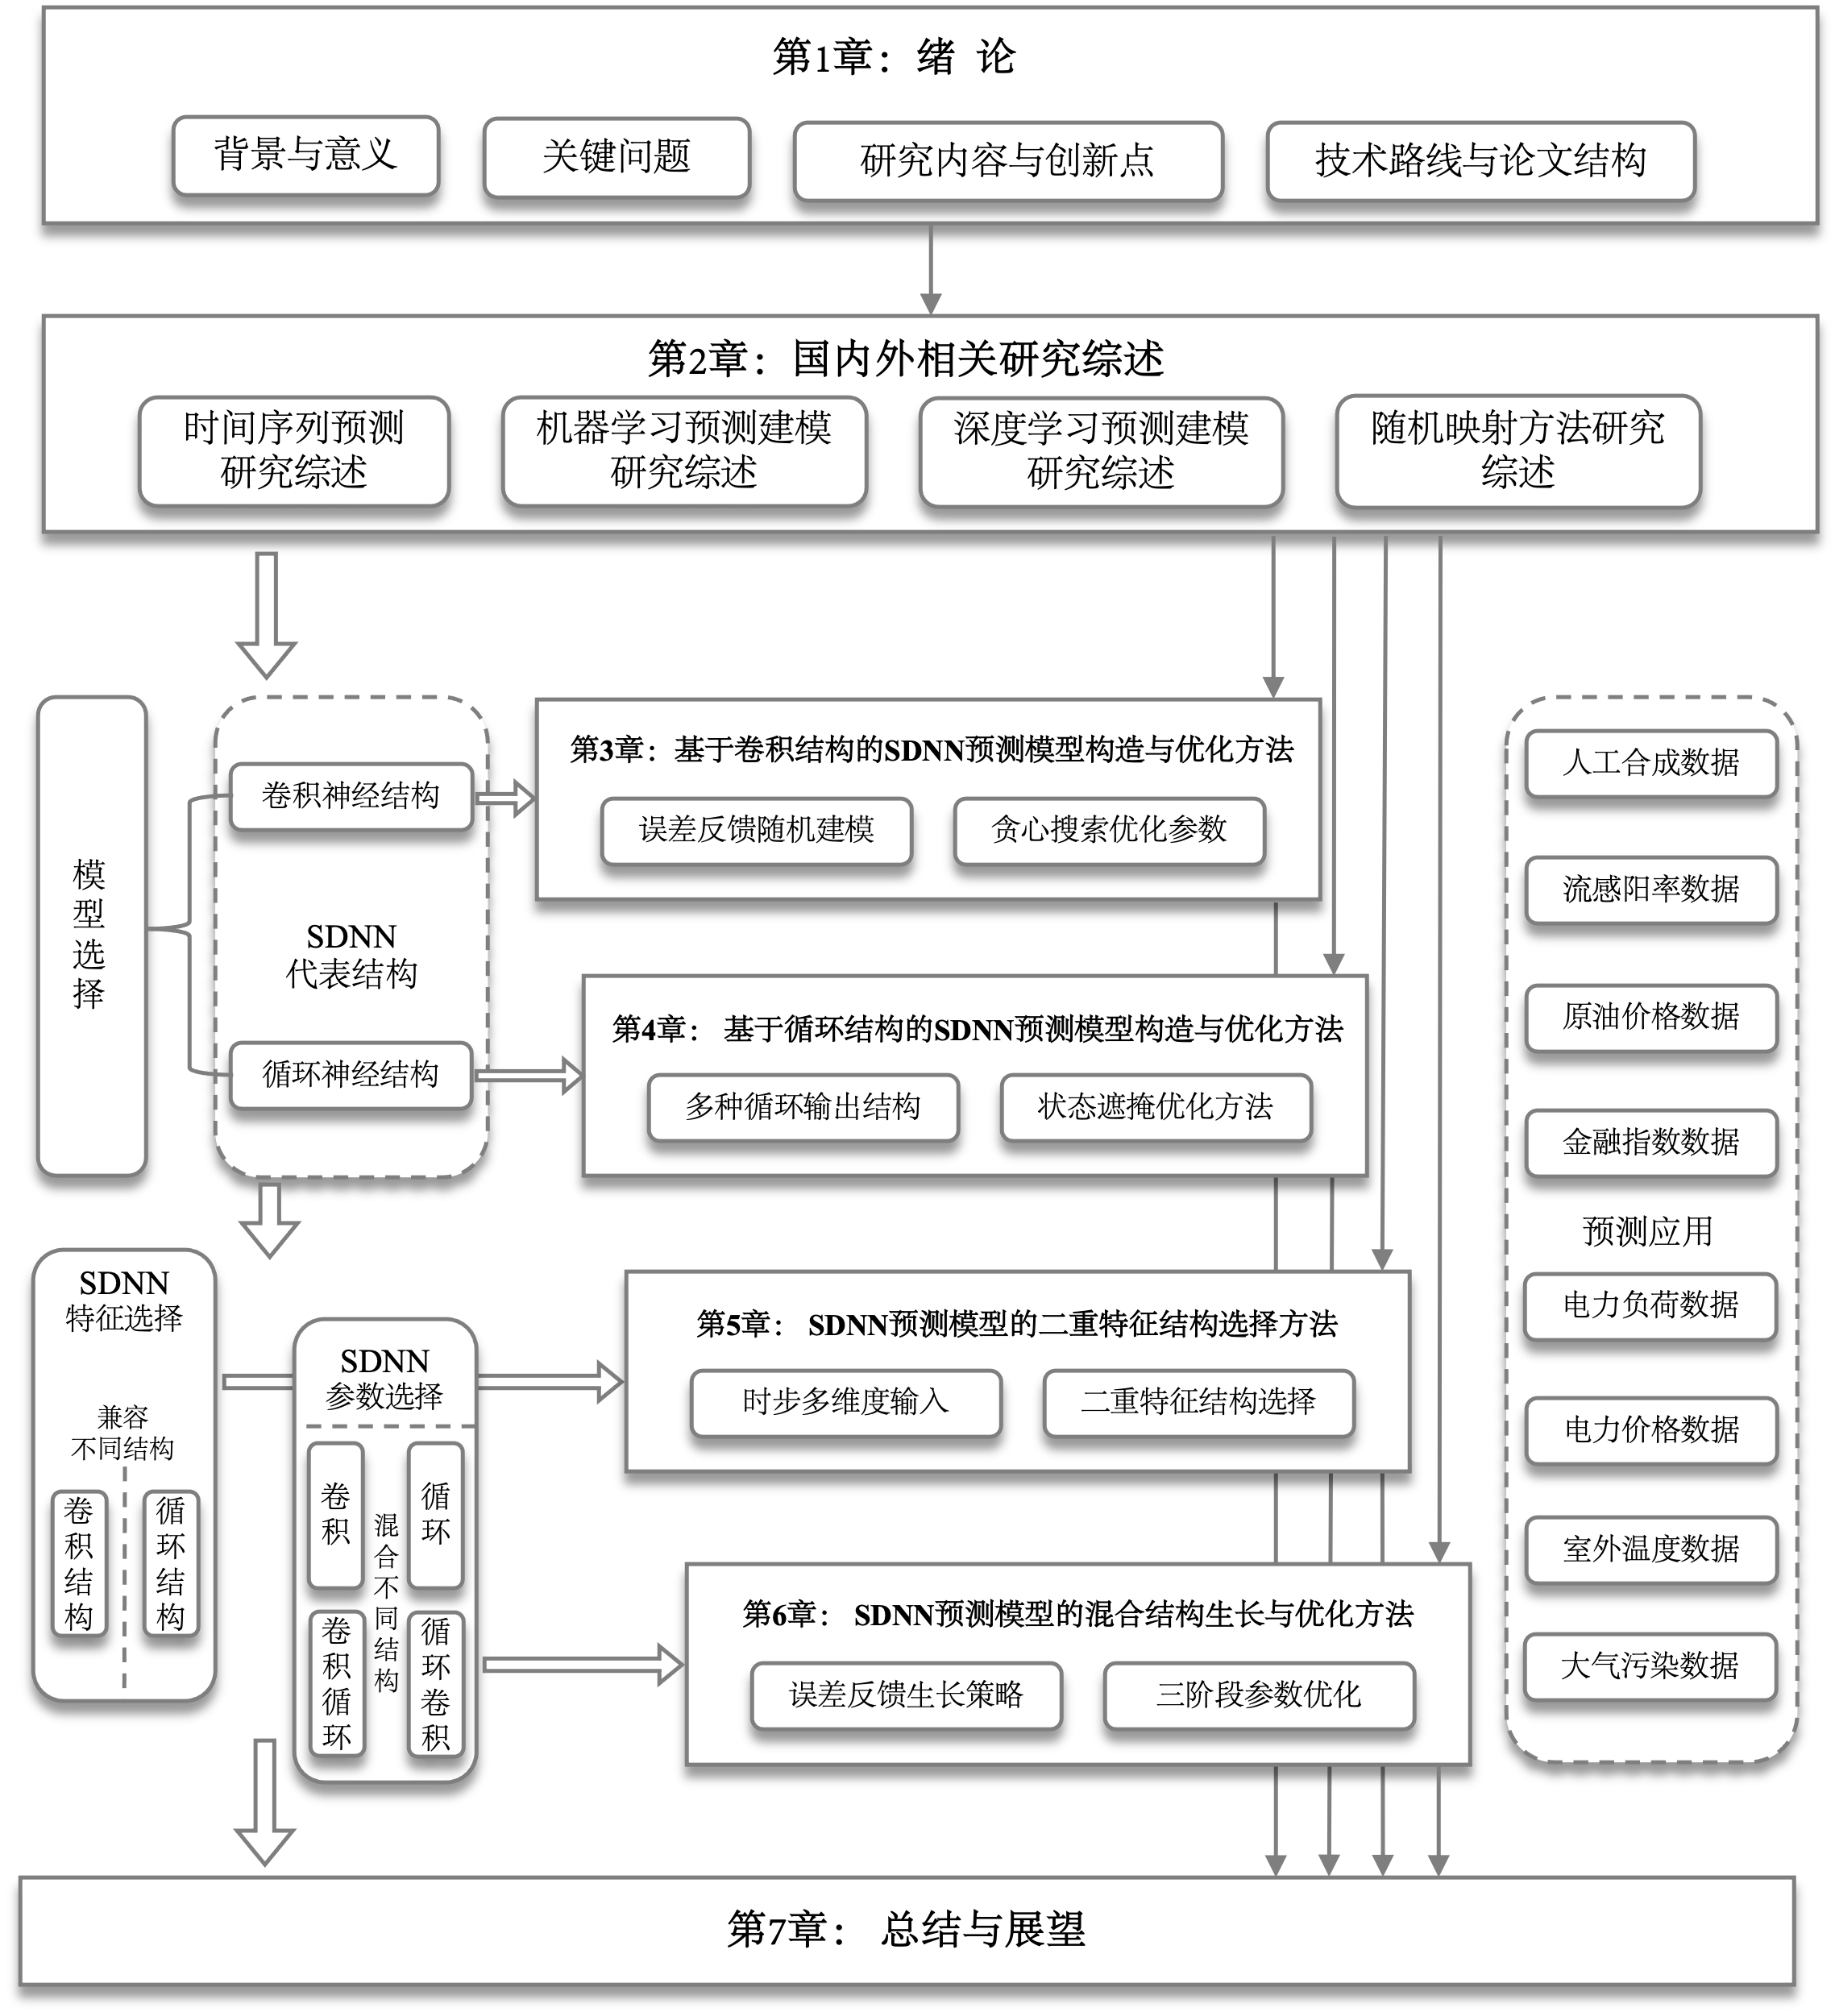
\includegraphics[width=0.95\linewidth]{float/ch.intro/thesis_content.png}
    \caption{\label{fig:body.arch}本论文主要结构}
\end{figure}

% \clearpage
\subsection{论文结构}
全文共七章,主要结构如\cref{fig:body.arch}所示,各章内容如下:

第1章~绪论:介绍了本研究的背景与意义、所面临的关键问题、主要的研究内容与创新点、研究内容间的技术路线及全文结构。

第2章~国内外相关研究综述:介绍了时间序列预测问题的定义、机器学习预测建模技术至深度学习预测建模技术的演进与现状、随机映射方法的动机及随机映射深度学习预测建模技术的现状及不足。

第3章~基于卷积结构的SDNN预测模型构造与优化方法:提出误差反馈随机建模构造方法及贪心搜索参数优化方法,建立出一种高效且收敛的卷积结构SDNN预测模型,结合人工合成数据、流感阳率数据、原油价格数据和金融指数数据的预测问题进行实验验证。

第4章~基于循环结构的SDNN预测模型构造与优化方法:考量多种随机映射循环输出结构及提出基于粒子群优化的状态遮掩优化方法,建立出一种改进的循环结构SDNN预测模型,结合人工合成数据、电力负荷数据和室外温度数据的预测问题进行实验验证。

第5章~SDNN预测模型的二重特征结构选择方法:构造兼容卷积结构与循环结构深度神经网络的时间序列数据二维输入特征结构及提出基于树状帕尔森估计的二重特征结构选择方法,建立出基于改进特征选择的SDNN预测模型,结合人工合成数据、电力负荷数据和电力价格数据的预测问题进行实验验证。

第6章~SDNN预测模型的混合结构生长与优化方法:改进误差反馈生长策略及提出子网络参数的三阶段优化方法,建立出一种准确、收敛且稳健的混合结构SDNN预测模型,结合人工合成数据、空气污染数据和电力负荷数据的预测问题进行实验验证。

第7章~总结与展望:总结本研究的主要内容、不足之处及改进方向。

其中,第3章至第6章为本文的主要研究内容章节,其逻辑关系在于以下方面:

(1)第3章与第4章为并列关系,该两章主要研究内容是第5章与第6章研究内容的基础。具体地,本研究聚焦基于随机映射的时间序列深度学习预测建模技术,卷积结构和循环结构作为既有深度神经网络的代表结构,本文第3章与第4章分别针对深度神经网络基于随机映射方法在特定于卷积结构和循环结构实现下的构造与优化问题展开研究,解决了既有卷积结构实现方法的性能瓶颈,改进了既有循环结构实现方法的输入输出映射,提升了在卷积结构和循环结构这类特定深度神经网络结构实现上的SDNN预测模型准确性。

(2)基于输入特征选择视角,第5章是对第3、4章内容的改进。具体地,凝练第3章与第4章所述SDNN卷积结构和循环结构对时步多维度输入能力的支持共性,设计了兼容卷积结构和循环结构的SDNN预测模型二重特征结构选择方法,突破了既有SDNN预测模型特征选择方法在一维输入结构上的局限,提升了基于卷积结构和循环结构的一般深度神经网络结构下的SDNN预测模型准确性。

(3)基于整体参数优化视角,第6章是对第3、4章内容的改进。具体地,将第3章与第4章所述SDNN卷积结构和循环结构作为超参数控制下的子网络结构状态,提出自适应混合多种不同特定类型子网络的SDNN预测生长策略,建立对子网络在生长过程中超参数、编码过程权重参数和生成过程权重参数的整体参数优化方法,进一步提升了自适应选择卷积结构和循环结构等混合深度神经子网络结构下的SDNN预测模型准确性。



% 第六章 总结与展望:本章对全文的研究工作进行总结,指出本文研究的不足和未来的展望。

% % \section{课题来源}
% % 本课题来源于:

% % 国家自然科学基金面上项目:基于多输出支持向量回归的预测技术研究(立项时间:2016-01,项目编号:71571080)。

% % 国家自然科学基金面上项目:大数据环境下基于计算智能的预测建模技术及其在电力负荷预测中的应用(立项时间:2019-01,项目编号:71871101)。

% % 国家电网公司华中分部科技项目:华中区域共享型电力交易与服务平台关键技术研究(立项时间:2020-03,项目编号:52140019000U)。
\chapter[国内外相关研究综述]{国内外相关研究综述}

\section{时间序列预测研究综述}
预测建模问题是气象水文~\cite{mudelseeTrend2019},公共卫生~\cite{chimmulaTime2020},电力系统~\cite{qiuEmpirical2017}和金融市场~\cite{niuDeveloping2020}等众多领域进行管理决策时的重要问题。例如,在电力系统的运行中,电力管理部门与发电企业需要预知未来时间的区域电力负荷、火电燃煤价格、风能光伏出力等信息,从而调整电力生产与配送电计划、燃料购买与存取用计划以及电力价格定价策略等决策,以确保电网安全、稳定、经济和高效的运行~\cite{hu2015jiyu};用电企业则需要预知未来的电力价格,从而调整工业生产计划,以降低企业用能成本,维持电力交易市场的稳定\cite{hongEnergy2020}。

如果能够建立一种模型以精准描述现实现象发生的规律,如构造区域电力负荷变化规律的确定性函数,则能够正确推算出未来的状态。然而,在复杂且动态的现实背景下,管理应用领域所关注的现象往往是不确定的,比如,经济的发展、天气的变化、甚至席卷世界的COVID19疫情波动等因素都会使得电力供需发生改变\cite{heHybrid2019,liuPower2022,obstAdaptive2021}。因此,种种未知因素的存在使得难以建立完备的因果关系来给出现象发生的定律,从而不可能建立出一个确定性的模型来精确计算现象的未来表现\cite{boxTime2011}。

尽管如此,依然有可能基于对现实现象的历史观测推导出一个模型,用来计算一定提前期的未来状态。这种基于现实现象自身的历史状态建立未来状态预测模型的方法被称为时间序列预测方法。其中,时间序列是指根据时间发生的历史先后顺序得到的序列形式数据观测值。众多管理领域的核心关注数据都是以时间序列的形式存在,例如气象水文领域中的温度时间序列、公共卫生领域中的流感阳性样本率时间序列、电力系统领域中的电力负荷时间序列和金融市场领域中的股票指数时间序列,等等。这类数据的典型特征便是相邻的观测值之间存在着相互依赖性。时间序列预测正是通过对时间序列观测值之间相互依赖性的分析,发展出动态模型,进而对时间序列的未来状态进行预测。

因此,时间序列预测的本质是一个以历史时间序列输入为自变量,以未来时间序列目标为因变量的函数逼近过程。
如Hewamalage et al.~\cite{hewamalageRecurrent2021}所定义的,时间序列预测问题可以被表示为如何基于过去时刻的时间序列观测值来生成未来时刻时间序列观测值的问题,具体如下:

给定一个历史T步的时间序列向量$\bm{x} = (x_1, \ldots, x_T)$,\(\x \in \mathr^{T}\),以及未来提前H步的时间序列向量$\bm{y} = (x_{T+1},\ldots,x_{T+H})$, \(\y \in \mathr^{H}\),时间序列预测问题可被公式化定义为:
\begin{equation}
    \mathcal{F} : f(\bm x) + \bm e = \bm y. \label{eq:sec.intro.def}
\end{equation}

\autoref{eq:sec.intro.def}中,$\mathcal{F}$是指时间序列预测模型所逼近的函数。\(f\)是指时间序列预测模型所学习出的预测函数,预测函数\(f\)基于历史$T$步内的时间序列观测值,生成提前$H$步的时间序列观测值\(\hat{\y} = f(\x)\)。$T$是历史的输入步长,$H$是未来的预测时长。\(\e\)表示模型的预测误差向量:\( \e = \y - \hat{\y} \),\(\e \in \mathr^{H}\)。

时间序列预测问题作为普遍存在于不同领域中的重要问题,成为了学术界与工业界长久以来的关注焦点,受到了诸多研究者和从业者的广泛重视。针对时间序列预测问题,已发展出了众多的时间序列预测建模技术。
传统的预测建模技术主要包括以自回归(Auto-regressive,AR)模型~\cite{boxTime2011}、移动平均(Moving average,MA)模型\cite{gershenfeldFuture1993}、自回归移动平均混合(Auto-regressive moving average,ARMA)模型\cite{chuForecasting2009}、整合移动平均自回归(Auto-regressive integrated moving average,ARIMA)模型\cite{floresEvolutive2012}和指数平滑(Exponential smoothing,ES)模型~\cite{gardnerjrExponential1985,gardnerExponential2006}等以统计学为基础的时间序列预测模型。这些模型通过构造历史观测值与相关因素的经验方程,对时间序列进行拟合和预测。例如,ARMA模型通过构造当前时刻滞后一定阶数的自回归项和误差累计项的线性组合,得到提前单步的预测值。
这些传统的预测建模方法通过分析特定领域的时间序列数据特征,建立出合适的预测函数,在一些时间序列预测问题中得到了成功应用。比如,Ediger et al.~\cite{edigerARIMA2007}应用ARIMA模型对土耳其2005年至2020年间的初级能源需求量进行了预测,并在结果中展示了ARIMA模型相对人工预测方法更高的准确度。
Chu\cite{chuForecasting2009}应用ARMA模型对亚太地区的游客数量进行了预测。
Christiaanse\cite{christiaanseShortTerm1971}针对短期电力负荷预测问题建立了一种基于ES的电力负荷预测模型。

然而,这些传统的统计预测方法往往将时间序列数据的输入输出映射视为预定义的函数,因此仅适用于某一特定类型的非平稳过程,而不能有效处理复杂非线性非平稳的时间序列预测问题\cite{boxTime2011}。
基于此,非线性预测的方法和技术成为时间序列预测建模研究中的热点。
其中,基于数据驱动的机器学习方法在时间序列建模预测领域备受关注。


\section{机器学习预测建模研究综述\label{sec:ch.intro.ml}}
对于时间序列预测问题,基于机器学习(Machine learning,ML)的预测建模技术一般是将该预测问题考虑为一种以历史T步的时间序列$\bm{x} = (x_1, \ldots, x_T)$为输入,以未来提前H步的时间序列$\bm{y} = (x_{T+1},\ldots,x_{T+H})$为输出的回归问题,进而构造监督机制下的回归模型予以求解。因此,对于基于机器学习的预测建模技术而言,其拟合过程可表示为:
\begin{equation}
    f(\bm x) + \bm e = \bm y, \quad f \in \{\vartheta, \theta\}\label{eq:sec.intro.ml}.
\end{equation}

\autoref{eq:sec.intro.ml}中,\(\theta\)表示机器学习预测模型的权重参数集合,\(\vartheta\)表示定义机器学习预测模型与权重学习机制的超参数集合。这里的超参数一般指代模型中权重参数以外的参数。针对不同的模型,\(\vartheta\)具有不同的内涵。例如,支持向量机(Support vector machine, SVM)模型中的\(\vartheta\)包含了核函数(Kernel function)的类型与参数、求解输出权重时的惩罚因子、误差松弛系数等参数,神经网络(Neural Network,NN)模型的\(\vartheta\)则包含了隐藏层的层数、每个隐藏层内神经元的数量以及激活函数的类型、权重训练方法的类型及其参数,等等。

概括而言,\(\vartheta\)定义了机器学习预测模型的结构以及权重参数的训练机制,\(\theta\)表示机器学习模型从输入变换到输出间的权重参数集合。在\(\vartheta\)与\(\theta\)的联合定义下,基于机器学习建模技术的时间序列预测模型\(f\)得以确定,即\(f \in \{\vartheta, \theta\}\)。

自然地,如何选择合适的\(\vartheta\)与\(\theta\)从而建立一个精准的预测模型\(f\)以降低模型预测误差,便是时间序列机器学习预测建模技术研究所关注的核心问题。
围绕此问题,涌现了大量的模型构造方法研究与模型优化机制研究。其中,以SVM和NN为代表的机器学习模型及其优化技术在时间序列建模问题中得到了广泛研究与应用。

在此,为更好介绍基于数据驱动的时间序列机器学习预测建模技术研究,以一组给定包含\(N\)个样本的时间序列数据\(\mathbb{D} = \left\{\left(\x_{n}, \y_{n}\right) \in\left(\mathbb{R}^{T} \times \mathbb{R}^{H}\right)\right\}_{n=1}^{N}\)为例,对基于SVM与NN的预测建模技术与应用展开概述。\(\left(\x_{n}, \y_{n}\right) \)表示第\(n\)个时间序列数据输入与输出的样本对。


\begin{figure}[t!]
    \centering
    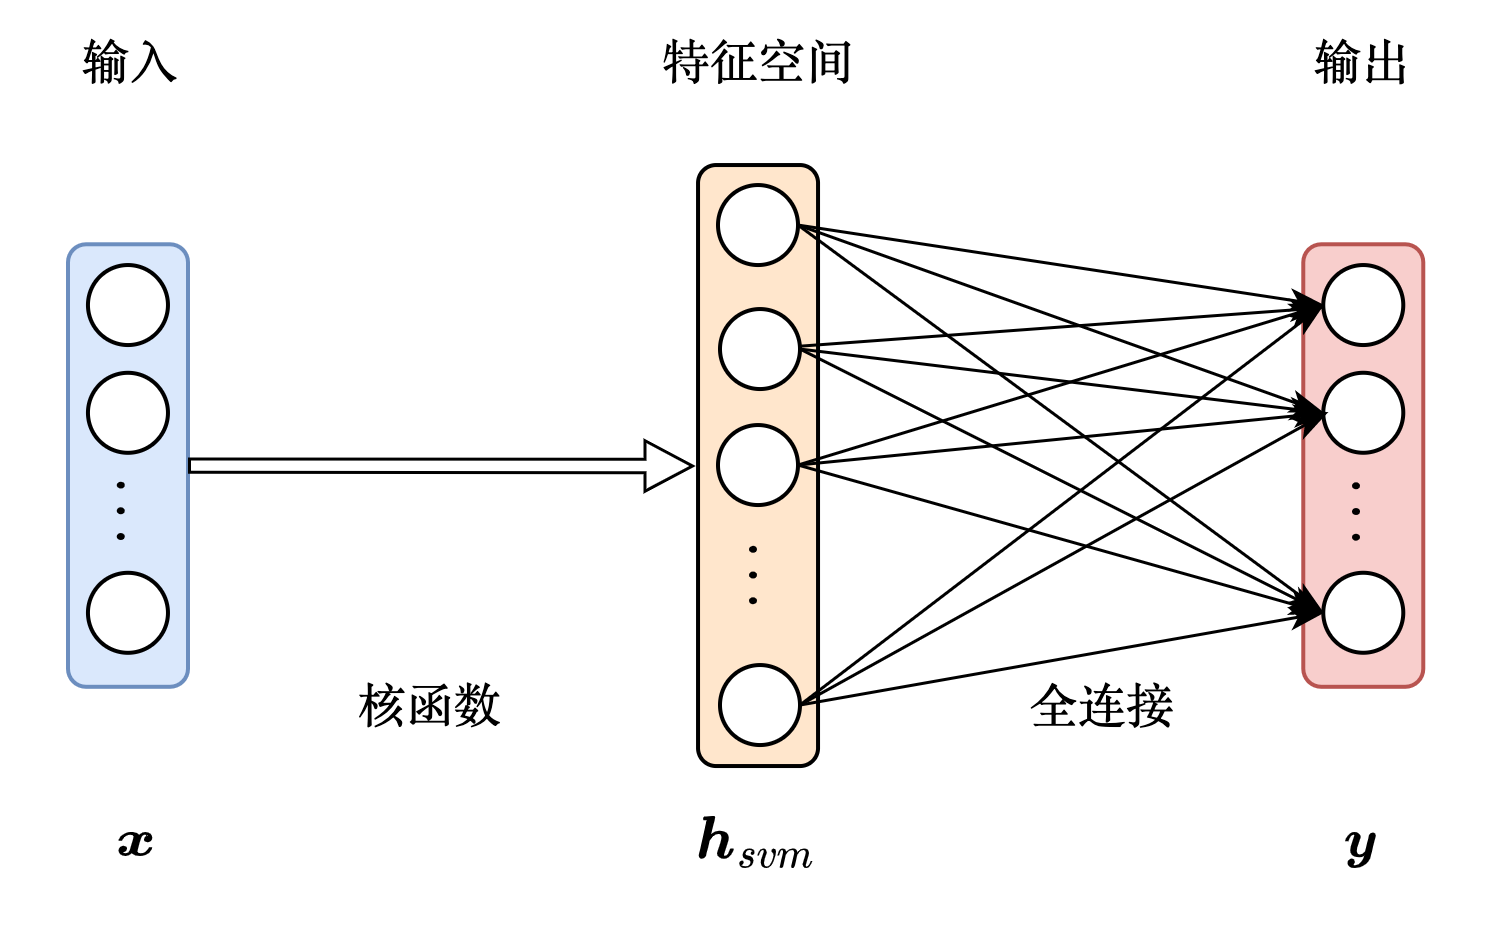
\includegraphics[width=0.8\textwidth]{float/ch.intro/svm.png}
    \caption{支持向量机结构示例\label{fig:ch.intro.svm}}
    % \setlength{\belowcaptionskip}{-10pt}
\end{figure}

\subsection{基于SVM的预测建模方法}
SVM是Vpanik~\cite{vapnikNature2013}基于统计学习理论所提出的一种机器学习方法,通过使用结构风险最小化原则代替传统的经验风险最小化原则,使其能较好解决有限样本的学习问题与过拟合问题。针对非线性不平稳的时间序列建模问题,如\autoref{fig:ch.intro.svm}所示,SVM预测模型通过引入核函数对非线性非平稳的时间序列输入特征\(\x\)进行核化,从而建立时间序列输入特征的高维特征空间表达\(\h_{svm}\),在求解输出权重时采用结合$L_2$正则化的合页损失(Hinge loss)实现结构风险最小原则,以此实现建模预测:
% \vspace{-4pt}
\begin{align}
    f_{svm}(\x) &= \w_{out}\h_{svm}, \label{eq:ch.intro.svmA} \\
    \h_{svm} &= \phi (\x)  \label{eq:ch.intro.svmC}.
\end{align}

\autoref{eq:ch.intro.svmA}中\(\w_{out}\)表示SVM预测模型的输出权重,\(\h_{svm}\)是SVM基于\autoref{eq:ch.intro.svmC}中核函数\(\phi(\cdot)\)所建立的特征空间状态表示。在经过以\(\mathd\)为训练集的核化后,\(\{\phi(\x_n)\}_{n=1}^N\)是一个维度为\(\mathr^{N\times N}\)的半正定(Positive semidefinite)矩阵,即有,\(\w_{out} \in \mathr^{H\times N}\)。
{\setlength{\abovedisplayskip}{12pt plus 3pt}
\setlength{\belowdisplayskip}{12pt plus 3pt}
\begin{equation}
    \w_{out} = \argmin_{\w_{out} }\left(\frac{\vartheta_{c}}{N}\sum^{N}_{n=1}\max(0, \left\lvert \y_n - f_{svm}(\x_n)\right\rvert  - \vartheta_{e}) + \frac{1}{2}\left\lVert \w_{out} \right\rVert^2\right)  .\label{eq:ch.intro.svmB}
\end{equation}
}

\autoref{eq:ch.intro.svmB}具体展示了SVM预测模型中\(\w_{out}\)通过$L_2$正则的合页损失予以求解的过程。\(\vartheta_{c}\)是指SVM的惩罚因子,用以调节合页损失与正则强度的平衡。\(\vartheta_{e}\)是指SVM的误差松弛系数,用以控制支持向量机的支持向量边界距离,从而增强SVM模型的鲁棒性。

显而易见,SVM预测模型中\(\w_{out}\)的求解问题是以约束条件为线性不等式组,目标函数为凸函数的问题。该问题是一个易于求解的典型二次规划问题。此外,对于时间序列数据\(\mathd\),一般\(N\)远大于\(T\)与\(H\)。由此,对于\(\{\x_n\}_{n=1}^N\)张成维度为\(N \times T\)的低维空间\(\mathbb{X} = \{\x_n\}_{n=1}^N \in \mathr^{N \times T}\)向由\(\{\y_n\}_{n=1}^N\)张成维度为\(N \times H\)的目标空间\(\mathbb{Y} = \{\y_n\}_{n=1}^N \in \mathr^{N \times H}\)的复杂非线性映射\(\mathcal{F}\)求解问题,SVM预测模型通过非线性核函数将其转变为高维特征空间\(\mathbb{H} := \{\phi(\x_n)\}_{n=1}^N \in \mathr^{N \times N}\)向低维空间\(\mathbb{Y}\)做线性映射的简单问题,同时利用\autoref{eq:ch.intro.svmB}中所展示的平衡性,具备了良好的预测性能。

因此,SVM预测模型具有高效、鲁棒、直接与参数易调整等特点,在时间序列预测建模研究中取得了广泛的关注和发展。例如,Fu et al.~\cite{fuEvolutionary2019}提出了一种基于SVM的人民币汇率预测模型;Hu et al.~\cite{huHybrid2015}针对短期电力负荷预测问题提出了一种基于SVM和混合特征提取策略的电力负荷预测模型;Tang et al.~\cite{tangNew2019}基于加权SVM提出了一种股票市场拐点预测模型;Xiong et al.~\cite{xiongCombination2015}将SVM模型与误差修正模型进行结合,提出了一种农产品价格预测模型。针对传统支持向量机的单步输出特点,面向时间序列的多步预测建模问题,Bao et al.~\cite{baoMultistepahead2014}基于传统的SVM模型提出了面向多步预测的多输出支持向量回归(Multiple-ouput support vector regression, MSVR)模型,并实验比较了传统单输出SVM模型与MSVR模型在不同多步预测策略(如迭代预测策略、直接预测策略和多输入多输出预测策略)下的性能表现。

针对时间序列预测建模任务下SVM的参数选择与模型选择问题,基于SVM收敛快,参数调整成本低等特点,Bao and Liu~\cite{baoFast2006}针对时间序列预测问题提出了一种基于快速网格搜索算法的SVM模型选择算法。在此基础上,Bao et al.~\cite{baoPSO2013}提出了基于粒子群优化(Particle swarm optimization,PSO)与模式搜索(Pattern search,PS)相结合的文化基因进化算法(Memetic algorithm,MA),并将其应用在SVM模型选择优化中。Hu et al.~\cite{huShortterm2016}利用PSO搜索SVM参数提出了一种基于PSO-SVM的预测模型。Hu et al.~\cite{huElectricity2013}提出了基于萤火虫算法(Firefly algorithm,FA)与PS算法相结合的MA算法,以此解决SVM电力负荷预测模型的模型选择问题。


\subsection{基于NN的预测建模方法\label{sec:ch.intro.nn}}
相较于SVM预测模型采用核函数方法进行非线性变换,且其输出权重具有闭式解的特点,基于神经网络的预测模型使用从输入层(Input layer)到隐藏层(Hidden layer)的非线性映射,对输入的非线性时间序列特征进行非线性变换,再由输出层(Output layer)对隐藏层表征的特征空间做线性组合进行预测输出。同时,基于神经网络的预测模型一般通过以均方误差(Mean square error,MSE)为损失函数(Loss function)的反向传播(Back propagation,BP)方式,通过梯度下降算法训练和优化神经网络各连接层(如输入层到隐藏层,隐藏层到隐藏层,隐藏层到输出层)的权重参数\(\theta\),从而实现预测建模~\cite{zhangSimulation2001}。

基于神经网络自身的结构特性,神经网络预测模型通过不同的神经网络隐藏结构构造方式以及网络权重参数训练方式衍生发展出了众多的变体。其中,多层感知机(Multilayer perceptron,MLP)作为一种以直接前馈(Feedforward)多层结构且层间均以全连接方式构造的神经网络,成为了机器学习方法下神经网络预测模型的代表结构。\autoref{fig:ch.intro.mlp}展示了一种经典的单隐藏层结构MLP模型。

\begin{figure}[t!]
    \centering
    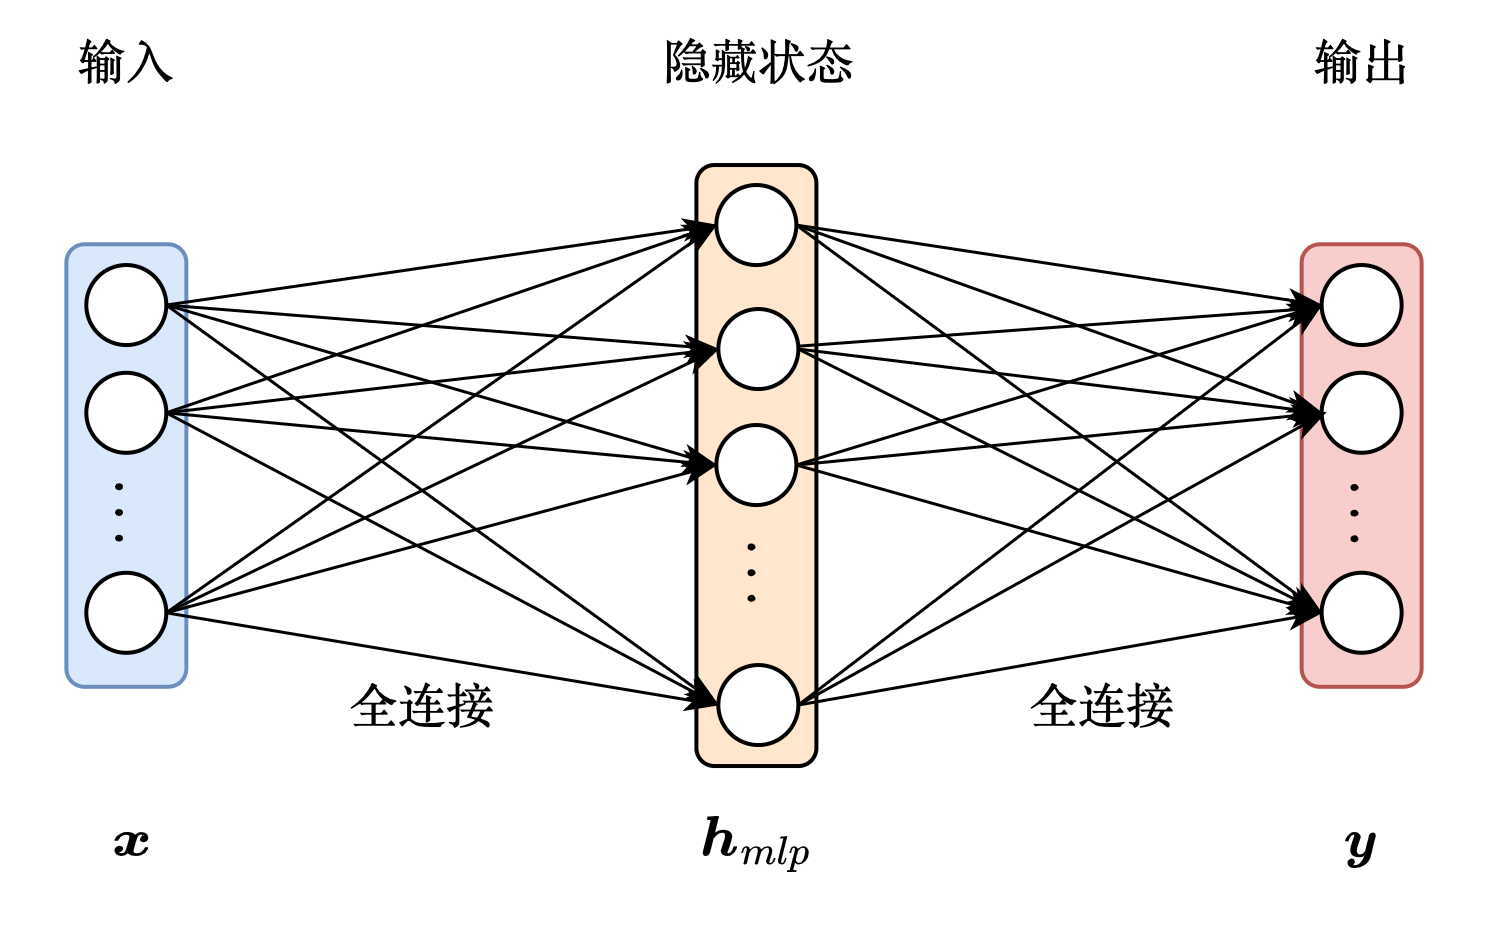
\includegraphics[width=0.8\textwidth]{float/ch.intro/mlp.png}
    \caption{多层感知机结构示例\label{fig:ch.intro.mlp}}
\end{figure}

以\autoref{fig:ch.intro.mlp}所示结构为例,其预测建模过程为:
\begin{align}
    f_{mlp}(\x) &= \w_{out}\h_{mlp}, \label{eq:ch.intro.mlpA} \\
    \h_{mlp} &= \sigma (\w_{hid}\x).  \label{eq:ch.intro.mlpB} 
\end{align}

\autoref{eq:ch.intro.mlpA}中\(\w_{out}\)同样表示模型的输出权重,\(\h_{mlp}\)是MLP通过\autoref{eq:ch.intro.mlpB}中激活函数\(\sigma(\cdot)\)对输入特征\(\x\)做非线性变换得到的隐藏层中隐藏状态状态表示。设该MLP模型中隐藏层神经元数量为\(K\),一般\(K\)大于 \(T\),远大于\(H\)。在经过训练集\(\mathd\)上的非线性变换后,使得低维输入空间\(\mathbb{X} = \{\x_n\}_{n=1}^N \in \mathr^{N \times T}\)至目标空间\(\mathbb{Y} = \{\y_n\}_{n=1}^N \in \mathr^{N \times H}\)的复杂非线性映射\(\mathcal{F}\)求解问题,通过隐藏层的非线性变换转变为高维特征空间\(\mathbb{H} := \{\sigma (\w_{hid}\x_n)\}_{n=1}^N \in \mathr^{N \times K}\)向低维空间\(\mathbb{Y}\)线性映射的简单问题。

通过对比\autoref{fig:ch.intro.mlp}与\autoref{fig:ch.intro.svm},以及对比\autoref{eq:ch.intro.mlpA}与\autoref{eq:ch.intro.svmA},可见MLP模型与SVM模型处理时间序列预测这一复杂问题的思路是一致。区别在于,SVM模型低维输入空间向高维特征空间变换是基于其\(\vartheta\)所定义的核函数,\autoref{eq:ch.intro.svmB}中输出权重的求解是闭式的;而MLP模型的特征空间变换是基于其\(\vartheta\)所定义的隐藏层结构与\(\theta\)所包含的隐藏层权重,且权重参数\(\theta:=\{\w_{out},\w_{hid}\}\)的优化问题是非凸的。

事实上,以MLP为代表,神经网络模型权重参数\(\theta\)的优化问题是普遍非凸的,且随着神经网络模型隐藏结构复杂程度的加深,例如隐藏层数的增加,而更加难以求解。针对此问题,基于反向传播(Back propagation,BP)的梯度下降(Gradient descent,GD)方法是一种有效且通行的方案。也因此,常有学者将基于梯度下降训练的神经网络模型称为反向传播神经网络(Back propagation neural network,BPNN)模型\cite{wangBack2015,wongTime1991,wangForecasting2011,dongSmall2018}。

其中,反向传播是指梯度下降训练方法中计算各层权重参数梯度时所使用的链式法则梯度传导过程。具体地,\(\theta\)的优化问题可以被视为以权重参数为自变量,以损失函数值为因变量,寻找合适的权重参数以找寻最小损失函数值的问题。设,\(\w\)表示权重参数集合\(\theta\)中的某一权重项,例如\autoref{eq:ch.intro.mlpA}中的输出层权重\(\w_{out}\)或\autoref{eq:ch.intro.mlpB}中的隐藏层权重\(\w_{hid}\),神经网络模型的损失函数为\(\ell(\w)\)。在经过以\(\mathd\)为训练集的神经网络预测模型表征后,一般有:
\begin{align}
    \ell(\w) &= \frac{1}{N \times H} \sum^N_{n=1} \|\e_{n}\| ,\label{eq:ch.intro.mse}\\
    \e_{n} & = \y_n - f(\x_n) \label{eq:ch.intro.en}.
\end{align}

\autoref{eq:ch.intro.mse}展示了神经网络预测模型在训练集\(\mathd\)上的MSE损失,其中,如\autoref{eq:ch.intro.en}所示,\(\e_n\)表示模型在训练集\(\mathd\)中第\(n\)个样本对上的预测误差向量,\(\norm{\e_n}\)是预测误差向量\(\e_n\)的$L_2$范数。

梯度下降方法的核心思想在于,基于神经网络中激活函数的连续性与可微性,通过向\(\w\)添加一个很小的动量\(\Delta_{\w}\),即\(\norm{\Delta_{\w}}\)很小,等价于\(\w + \Delta_{\w}\)近似\(\w\),利用泰勒近似将复杂非凸的\(\ell(\w)\)函数优化问题当作一个简单的函数极小值求解问题。其中,\(\ell({\w + \Delta_{\w}})\)可用一阶泰勒展开予以近似:
\begin{equation}
    \ell({\w + \Delta_{\w}} ) \approx \ell({\w}) +  \nabla_{\w}^\trans \Delta_{\w}. \label{eq:ch.intro.gd}
\end{equation}

\autoref{eq:ch.intro.gd}中,\(\nabla_{\w}\)表示\(\w\)在误差函数\(\ell\)中的梯度。此时,梯度下降方法的目标便是找寻合适的动量\(\Delta_{\w}\)使得\autoref{eq:ch.intro.gd}中损失函数\(\ell\)最小。在最陡下降中,定义学习速率(Learning rate)为\(\eta \),且\(\eta  > 0\),令:
\(\Delta_{\w} = -\eta \nabla_{\w}\)。
则有如\autoref{eq:ch.intro.eta}所示不等式性质:
\begin{equation}
\ell({\w}) > 0 \quad \text{且} \quad \eta  \nabla_{\w}^\trans \nabla_{\w} > 0. \label{eq:ch.intro.eta}
\end{equation}

当\(\eta \)足够小时,\autoref{eq:ch.intro.gd}的条件得到满足,即可直接证明出如\autoref{eq:ch.intro.lr}所示收敛性质:
\begin{equation}
    \ell({\w -\eta \nabla_{\w}} ) \approx \ell({\w})  -\eta  \nabla_{\w}^\trans \nabla_{\w} < \ell({\w}). \label{eq:ch.intro.lr}
\end{equation}


\begin{algorithm}[t!]
    \caption{神经网络模型梯度下降方法训练过程}
    \renewcommand{\algorithmcfname}{算法}
    \renewcommand{\algorithmicrequire}{\textbf{输入:}}
    \renewcommand{\algorithmicensure}{\textbf{输出:}}
    \label{alg:ch.intro.gd}
    \begin{algorithmic}[1]
        \REQUIRE {数据集\(\mathd= \left\{\left(\x_{n}, \y_{n}\right) \in\left(\mathbb{R}^{T} \times \mathbb{R}^{H}\right)\right\}_{n=1}^{N}\),神经网络模型超参数集合\(\vartheta\)
        }
        \REQUIRE {
            基于设定的神经网络模型超参数集合\(\vartheta\),初始化如下参数:\\
            梯度下降方法的当前迭代次数\(i\leftarrow 0\)\\
            当前迭代次数下神经网络权重参数集合\(\theta^i\)\\
            与模型训练相关的其他参数
        }
        \ENSURE{神经网络模型权重参数集合\(\theta\),神经网络模型超参数集合\(\vartheta\),确定神经网络模型\(f \in \{\vartheta, \theta\}\)
        }
        \WHILE{未满足\(\vartheta\)界定的收敛条件}
        \STATE \(i\leftarrow i+1\)
        \STATE 基于\(\theta^i\),确定模型\(f \leftarrow  f \in \{\vartheta, \theta^i\}\)
        \STATE 基于数据集\(\mathd\)和模型\(f\),完成前馈过程\(f(\x)\),计算模型损失函数值\(\ell({\w}) \)
        \FOR{\(\w\) in \(\theta^i\) }
        \STATE 选取计算梯度所需的样本
        \STATE 根据反向传播链式法则计算梯度信息\(\nabla_{\w}\)
        \STATE 根据梯度下降更新公式更新权重参数\(\w\)
        \ENDFOR
        \ENDWHILE
        \RETURN {
            已完成更新过程的权重参数集合\(\theta \leftarrow \theta^i\)
        }
    \end{algorithmic}
    \medskip
\end{algorithm}

同时,借助从输出层向输入层的反向传播过程,通过链式法则可以依次计算出输出端至输入端所有权重参数的局部梯度,
从而完成模型权重参数集合\(\theta\)内所有权重参数的单次更新。完整的神经网络预测模型训练过程如算法\ref{alg:ch.intro.gd}所示。

显然,梯度下降方法的性能与效率直接决定了基于梯度下降方法训练权重参数的神经网络模型性能与建模效率~\cite{liuImproved2020}。因此,神经网络梯度下降方法的改良问题成为了神经网络建模技术研究中的重要问题。围绕此问题,已发展出了众多梯度下降改进方法。
例如,基于牛顿法的梯度下降方法~\cite{bennettNewton1916}将凸优化中的牛顿法(Newton method)引入非凸的神经网络权重参数优化问题中,通过将\autoref{eq:ch.intro.gd}中的一阶泰勒近似调整为二阶泰勒近似,加速了神经网络模型的收敛速度\cite{nesterovMethod1983a,nesterovCubic2006}。
随机梯度下降(Stochastic gradient descent,SGD)方法~\cite{bottouStochastic2012}则通过将\autoref{eq:ch.intro.mse}中基于完整训练集的损失函数计算方式修改为基于随机选取的单个样本来计算损失函数值,从而大大降低了梯度下降方法的计算复杂度。
为抑制SGD方法随机选取样本所带来的梯度震荡,Sutskever et al.~\cite{sutskeverImportance2013}引入了动量(Momentum)的概念,通过向\autoref{eq:ch.intro.gd}中的梯度向量添加动量,使得模型权重参数向相关方向加速变换,从而实现加速收敛。
针对\autoref{eq:ch.intro.lr}中学习速率的选择问题,Duchi et al.~\cite{duchiAdaptive2011}提出了自适应梯度法(Adaptive gradient algorithm,AdaGrad),通过对较为密集的特征设置较小的学习速率,对较为稀疏的特征设置较大的学习速率,从而实现了针对特征的学习速率自适应设置。

% \raggedbottom
概括而言,尽管这些梯度下降方法的细节各有不同,但基于梯度下降方法的神经网络模型总体遵循算法\ref{alg:ch.intro.gd}中所示的输入、输出与执行步骤完成模型的参数优化。由此,通过梯度下降方法的权重参数训练,机器学习方法下的神经网络预测模型具备了良好的预测性能。

其中,前文所举例的MLP预测模型凭借其神经网络结构相对简单,权重参数较易训练,可通过构造具有多个神经元的输入层与输出层自然实现多输入多输出(Multiple-input Multiple-output,MIMO)策略等特点,被广泛应用于时间序列预测建模任务,尤其是提前多步预测的预测建模任务中。例如,Hamzaçebi et al.~\cite{hamzacebiComparison2009}比较了MLP在多步时间序列预测任务中采用直接策略与迭代策略的性能差异。相对于以往采用单一MLP进行多步预测的方法,Adeodato and Monteiro~\cite{adeodatoMLP2011}提出了一种基于集成思想的多步预测方法,通过集成多个MLP进行多步时间序列预测,从而提升了预测精度。
Flores et al.~\cite{floresEvolutive2012}通过遗传算法(Genetic algorithm,GA)对MLP中的隐藏层单元数、激活函数的种类进行优化,提出了一种基于GA-MLP的预测方法。
Bao et al.~\cite{baoPSOMISMO2014}针对时间序列的多步预测问题,以MLP作为预测模型,提出了一种基于PSO的多输入子多输出时间序列预测建模策略,更进一步地提升了多层感知机在时间序列多步预测上的性能。针对流感预测问题,Yang and Bao~\cite{yangComprehensive2021}通过实验表明了在多输入多输出策略、直接策略和迭代策略以及MLP预测模型和MSVR模型的策略与模型两两组合中,基于MIMO策略的MLP模型和MSVR模型具备更高的预测精度。
% \clearpage

\section{深度学习预测建模研究综述}
\subsection{深度学习建模方法}
近年来,得益于海量数据的积累、计算设备浮点运算能力的大幅提升、梯度下降方法的改进、以及通用神经网络建模框架(如Google推出的Tensorflow~\cite{abadiTensorflow2016},Meta\footnote{曾用名Facebook。Facebook于2021年10月改名为Meta。}推出的Pytorch~\cite{paszkePytorch2019}和Microsoft推出的CNTK~\cite{seideCNTK2016}等)的出现与推广,以卷积神经网络(Convolution Neural Network,CNN)~\cite{li2016juanji}和循环神经网络(Recurrent Neural Network,RNN)~\cite{yang2018xunhuan}为代表结构的深度学习(Deep learning,DL)建模技术受到了学术界和工业界的广泛关注和研究。

深度学习建模技术是机器学习建模技术中一类基于深度神经网络(Deep neural network,DNN)的建模技术\cite{lecunDeep2015}。其中,DNN是对基于不同深度神经结构所构建的神经网络的统称。例如,基于卷积结构的CNN和基于循环结构的RNN均属于DNN,其是DNN在不同特定结构上的具体实现。

深度学习建模技术与传统机器学习建模技术之间的区别在于,针对一些复杂场景的建模问题,例如计算机视觉(Computer vision,CV)中的图像分类问题\cite{dengImageNet2009}和自然语言处理(Natural language processing,NLP)中的文本分类问题\cite{maasLearning2011},传统的机器学习建模技术受限于简单的模型结构,在原始输入特征的基础上难以直接取得较好的分类结果,因此往往需要人工经验建立特定的特征提取方法,如基于图像像素数值高斯分布(Gaussian distribution)描述图像特征的Fisher Vector方法\cite{sanchezHighdimensional2011,sanchezImage2013,perronninLargescale2010}和基于语言文档内词频信息描述语句特征的词频-逆文档(Term frequency - inverse document frequency,TF-IDF)方法\cite{aizawaInformationtheoretic2003,jonesStatistical1972,luhnStatistical1957},从原始数据输入特征中提取出新的特征以提升机器学习模型处理这些问题的能力。而深度学习建模技术则直接将原始数据特征作为输入,依靠DNN的神经网络结构,如CNN中的卷积结构和RNN中的循环结构,在模型权重参数的训练中学习出数据的特征表示,成功增强了模型对于问题理解能力与解决能力。

\begin{figure}[t!]
    \centering
    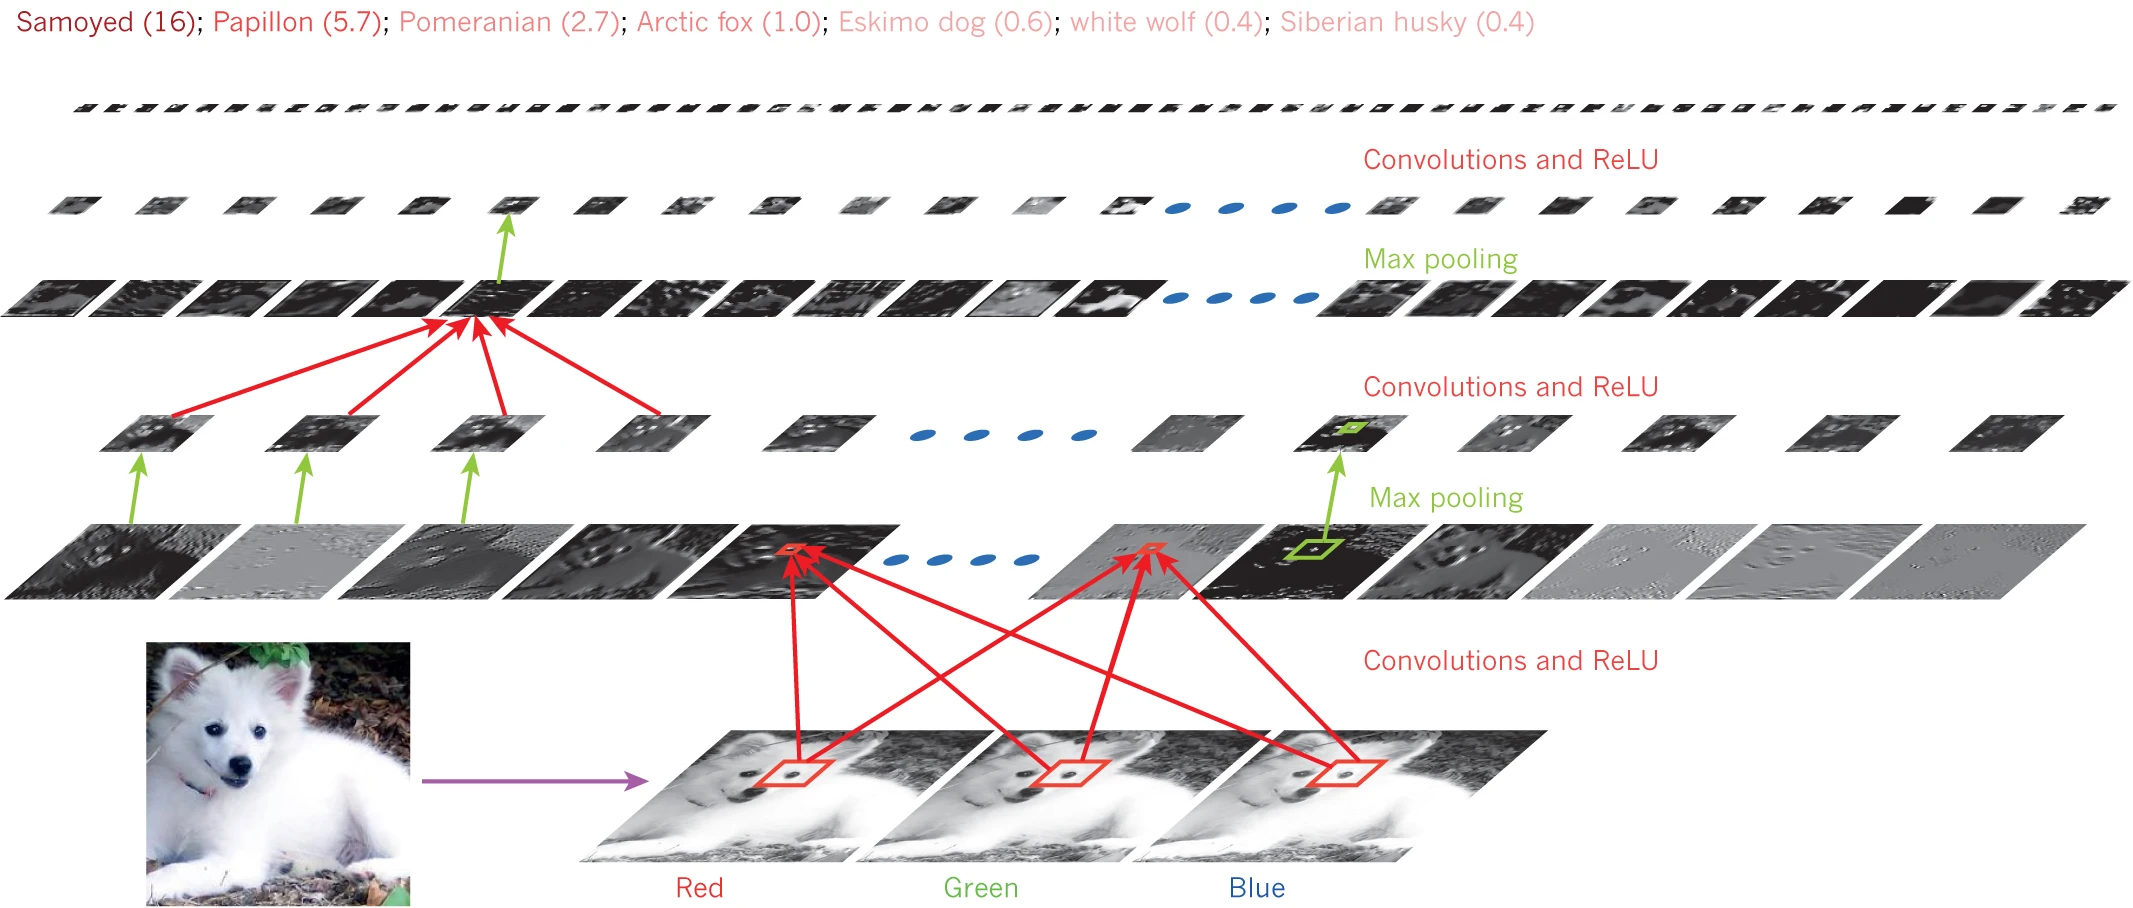
\includegraphics[width = \linewidth]{float/ch.intro/lecun.png}
    \caption{卷积神经网络图像分类模型示例(引用于Lecun et al. Deep Learning. Nature, 2015, 521(7553): 436-444,详见文献~\cite{lecunDeep2015})} 
    \label{fig:ch.intro.lecun}
\end{figure}

\autoref{fig:ch.intro.lecun}通过引用Lecun等\cite{lecunDeep2015}在Nature期刊上的CNN图像分类模型示例,形象展示了CNN基于卷积结构逐层学习图像特征表示的过程。其中,红色线表示卷积层(Convolutional layer)的卷积操作,绿色线表示池化层(Pooling layer)的下采样操作,图底处的“Red”、“Green”和“Blue”分别表示彩色图片在红绿蓝三原色下的数值状态,图顶处“Samoyed(16)”等信息展示出模型在各图片类别上的置信度,基于置信度信息,可知模型成功分类出了图片所展示的萨摩耶犬种类别。

作为在图像处理和自然语言处理等领域表现出优异性能的深度神经网络~\cite{alomStateoftheart2019},CNN与RNN在时间序列预测建模任务上的应用也成为了近年来的研究热点~\cite{sezerFinancial2020,lindbergLongterm2019,mudelseeTrend2019}。例如,Sadaei et al.~\cite{sadaei2019short}提出了一种基于CNN的短期负荷预测模型,通过将多变量的时间序列以图像的形式加以封装,使其作为输入来训练CNN预测模型,实验展示了该CNN负荷预测模型的优异性能。Salinas et al.~\cite{salinasDeepAR2020}对长短期记忆(Long-short term memory,LSTM)神经网络这一具有门控(Gate)机制的RNN加以改进,提出了一种名为深度自回归(Deep autoregression,DeepAR)的时间序列多步概率预测模型。Wang et al.~\cite{wangPhotovoltaic2019}将CNN与LSTM结合,通过LSTM对时间序列数据的长短期特征进行特征学习和表达,而后基于CNN对LSTM结构的表征在空间特征上进行学习,提出了一种长短时记忆卷积神经网络结构的深度时间序列预测模型,并结合光伏发电预测任务开展应用研究。



\subsection{模型选择问题}

\begin{algorithm}[t!]
    \caption{基于梯度下降方法的神经网络预测建模技术模型选择过程}
    \renewcommand{\algorithmcfname}{算法}
    \renewcommand{\algorithmicrequire}{\textbf{输入:}}
    \renewcommand{\algorithmicensure}{\textbf{输出:}}
    \label{alg:ch.intro.ms}
    \begin{algorithmic}[1]
        \REQUIRE {数据集\(\mathd= \left\{\left(\x_{n}, \y_{n}\right) \in\left(\mathbb{R}^{T} \times \mathbb{R}^{H}\right)\right\}_{n=1}^{N}\),神经网络模型超参数集合\(\vartheta\)的搜索空间\(\Omega\)
        }
        \REQUIRE {
            基于设定的超参数搜索空间\(\Omega\),初始化如下参数:\\
            模型选择方法的当前迭代次数\(j\leftarrow 0\)\\
            当前迭代次数下最优的神经网络超参数集合\(\vartheta^*\)\\
            当前迭代次数下最优的神经网络权重参数集合\(\theta^*\)\\
            与模型选择相关的其他参数
        }
        \ENSURE{神经网络模型权重参数集合\(\theta\),神经网络模型超参数集合\(\vartheta\),确定神经网络模型\(f \in \{\vartheta, \theta\}\)
        }
        \WHILE{未满足模型选择方法界定的收敛条件}
        \STATE \(j\leftarrow j+1\)
        \STATE 从超参数集合\(\vartheta\)的搜索空间\(\Omega\)中选择或更新出当前的超参数集合\(\vartheta^j\)
        \STATE 基于\(\vartheta^j\):\\
        \hspace{2em}执行算法\ref{alg:ch.intro.gd}所示步骤\\
        \hspace{2em}得到当前\(\vartheta^j\)试验下的权重参数集合\(\theta|\vartheta^j\)\\
        \hspace{2em}确定模型\(f \leftarrow  f \in \{\vartheta^j, \theta|\vartheta^j\}\)
        \STATE 基于数据集\(\mathd\)和模型\(f\),计算模型误差
        \STATE 基于模型误差与超参数更新方法:\\
        \hspace{2em}更新最优的神经网络超参数集合\(\vartheta^*\)\\
        \hspace{2em}更新最优的神经网络超参数集合\(\theta^* \leftarrow  \theta|\vartheta^*\)
        \ENDWHILE
        \RETURN {
            已完成更新过程的超参数集合\(\vartheta \leftarrow \vartheta^*\)与权重参数集合\(\theta \leftarrow \theta^*\)
        }
    \end{algorithmic}
\end{algorithm}
尽管深度学习预测建模技术在一些时间序列建模预测任务中表现出了优秀的学习能力,但在面对具体应用问题时,深度学习预测建模技术仍然会遇到建模技术所普遍面临的模型选择(Model selection)问题。具体地,模型选择问题是指,针对一个应用问题,如何找寻合适的模型参数以优化该模型性能的问题\cite{guyonModel2010,hastieElements2009,escalanteParticle2009}。

在本文所关注的时间序列预测问题中,如\autoref{eq:sec.intro.def}所示,对于由超参数集合\(\vartheta\)和权重参数集合\(\theta\)所定义的NN预测模型\(f\),其模型选择问题便是如何选择合适的\(\vartheta\)与\(\theta\)从而提升模型\(f\)预测性能的问题。具体地,模型选择过程如算法\ref{alg:ch.intro.ms}所示。

其中,权重参数集合\(\theta\)是基于算法\ref{alg:ch.intro.gd}所示的梯度下降训练方法予以确定。但如算法\ref{alg:ch.intro.gd}中的输入所示,权重参数集合\(\theta\)依赖于超参数集合\(\vartheta\)所定义的模型神经网络结构参数(如CNN模型中卷积层层数、卷积核宽度和卷积核数量等等)和梯度下降方法参数(如SGD方法中的学习速率、批次样本选取数量和动量惯性系数等等),不同的\(\vartheta\)必然会导致\(\theta\)的差异。因此,作为一类梯度下降方法训练的神经网络建模技术,基于DNN的深度学习预测建模技术在处理模型选择问题时同样需要遵循如算法\ref{alg:ch.intro.ms}所示的模型选择过程。

% \begin{figure}[t!]
%     \centering
%     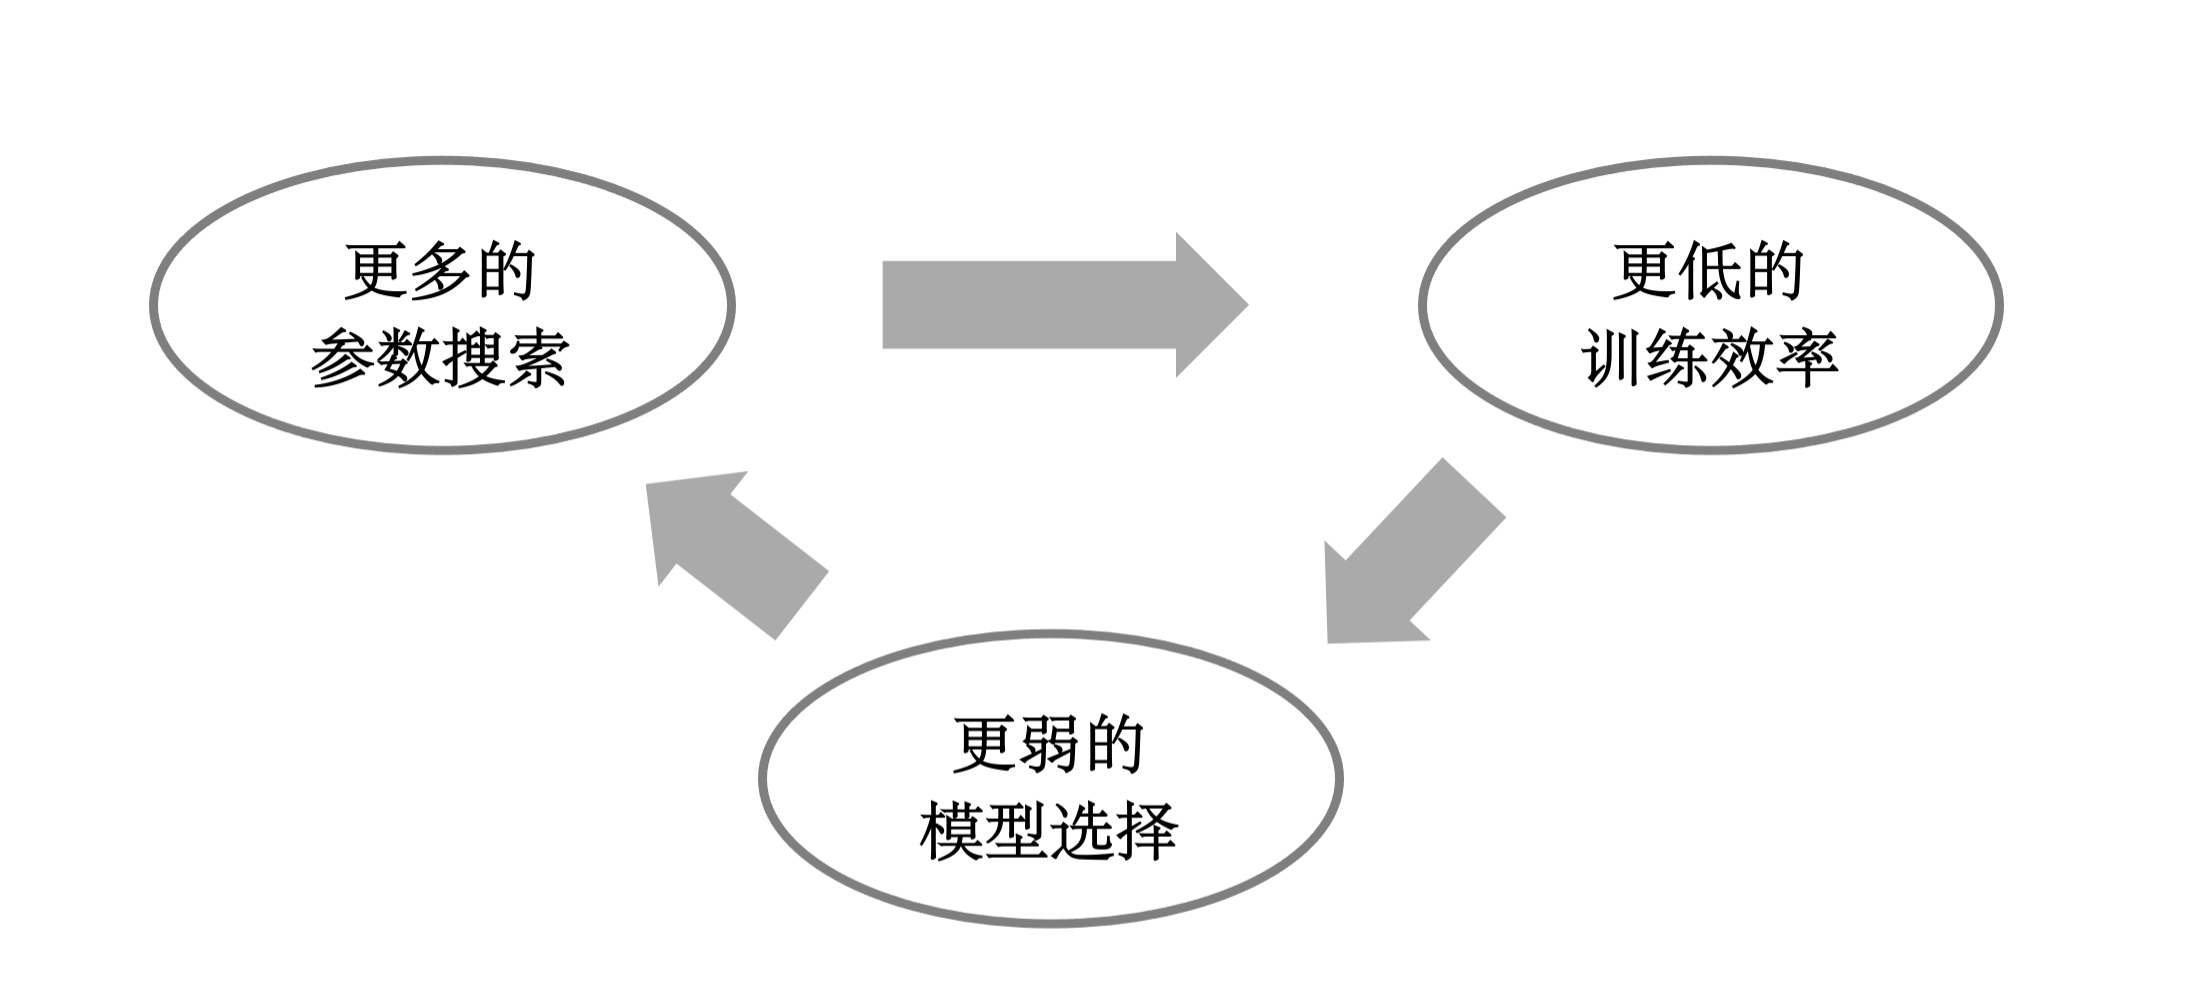
\includegraphics[width = \linewidth]{float/ch.intro/DL.png}
%     \caption{深度学习预测建模技术的模型选择挑战} 
%     \label{fig:ch.intro.dl_c}
% \end{figure}

与传统机器学习预测建模技术所遇到的模型选择挑战不同,深度学习预测建模技术所面临的模型选择挑战尤为突出。深度学习模型复杂的神经网络构型使其在实际应用时难以选择出合适的神经网络结构\cite{miikkulainenChapter2019}。这里的困难主要体现在两个方面:一是相较以MLP为代表的浅层简单结构神经网络模型,深度学习模型往往因其更深的隐藏结构而具有更多的权重参数以及更加复杂的梯度计算方式,降低了算法\ref{alg:ch.intro.ms}中步骤4所示的权重参数优化效率\cite{glorotUnderstanding2010,pascanuDifficulty2013},从而导致了深度神经网络预测建模技术模型选择效率低的问题;二是复杂的神经网络结构加深了算法\ref{alg:ch.intro.ms}中超参数搜索空间\(\Omega\)的复杂程度,从而导致了深度神经网络预测建模技术神经网络结构选择效果差的问题。尤其,
% 如\autoref{fig:ch.intro.dl_c}所示,
较低的权重参数优化效率会再次增加神经网络结构选择的难度,神经网络结构难度的加大会进一步降低模型选择的效率。


因此,在本文所聚焦的时间序列预测建模问题中,深度学习预测建模技术梯度下降方法效率低、神经网络结构复杂所导致的模型选择效果差的问题使得当前时间序列深度学习预测建模技术应用存在较大局限。这些问题大大增加了优化时间序列深度学习预测模型所需的计算时间、计算资源和人员精力,使得现实任务中的深度学习预测模型难以被精细优化,进一步限制了时间序列深度学习预测模型的准确性、稳定性、可靠性和应用性。其中,梯度下降方法是造成深度学习预测建模技术模型选择效率低下的主要因素。尽管已有众多提高梯度下降过程效率的方法\cite{bottouStochastic2012,duchiAdaptive2011,liuImproved2020},但如\autoref{sec:ch.intro.ml}中所述,这些方法仍需遵循算法\ref{alg:ch.intro.gd}中所示步骤,多次迭代计算梯度以渐进优化权重参数的本质没有改变。因此,基于梯度下降方法的深度学习预测建模技术从根源上便存在模型选择效率低的问题,在改变试验超参数时始终需要重新训练权重参数才可得到当前超参数的模型效果,其模型选择的效率难以显著降低。因而,现有的时间序列深度学习预测建模技术模型选择研究多集中于神经网络结构选择问题的研究。


时间序列深度学习预测技术中的神经网络结构选择问题是指,根据时间序列预测任务的场景如何选择合适的深度神经网络结构以实现更优的预测性能。
根据深度学习模型预测建模过程的阶段可以将神经网络结构选择问题分解为深度学习模型的表征结构选择问题与输出结构选择问题。
时间序列深度学习预测模型表征结构与输出结构分别是指深度学习模型对时间序列数据输入特征进行深层非线性表征的神经网络结构,以及对深层非线性表征结果进行解码以生成输出结果的神经网络结构。
前者具体如,CNN的输入层(Input layer)、卷积层(Convolutional layer)与池化层(Pooling layer)结构~\cite{koprinskaConvolutional2018},RNN的输入层和隐藏层(Hidden layer)结构~\cite{salinasDeepAR2020}等;而后者具体如,基于全连接层(Fully connected layer)的解码器结构~\cite{koprinskaConvolutional2018,caiDayahead2019},基于循环结构的解码器结构~\cite{liuDSTPRNN2020}
和自回归结构~\cite{caiDayahead2019,salinasDeepAR2020}等。其中,CNN预测模型因其神经网络结构的前馈机制,一般采用全连接解码器结构作为其输出结构;而RNN预测模型因其神经网络的循环机制,衍生出包括全连接结构解码器、循环结构解码器和自回归结构在内的多种输出结构。因此,表征结构的选择问题是CNN预测建模技术与RNN预测建模技术的共性问题,而输出结构的选择问题是基于RNN建模技术的深度学习预测模型特有问题。同时,RNN预测建模技术可通过调整解码器结构自然地实现不同的多输出生成策略。因此,对于基于RNN的DNN预测模型而言,时间序列预测中的多输出选择问题是其神经网络结构选择问题中的一类特定问题,表现为输出结构的选择问题。

此外,深度学习模型的表征结构可进一步细分为输入结构与隐藏结构。对基于神经网络的预测建模技术而言,因其输出层单元与时间序列多输入特征的一一对应,神经网络预测建模技术输入结构的选择直接反映了输入特征的选择。例如,Sezer and Ozbayoglu~\cite{sezer2018algorithmic}利用CNN卷积核的多通道输入能力,将金融时间序列转换为二维输入结构,以此构造基于CNN的算法交易模型。Yang et al.~\cite{yangShortterm2021}借助扩充RNN的输入层结构将传统的单变量时间序列预测建模多输入策略加以优化,使其从传统的单个输入时步对应单个输入观测值扩充为了单个输入时步对应连续多个输入观测值,通过PSO算法优化输入步长进一步提高了RNN预测模型的准确率。因此,DNN预测建模技术的特征选择问题亦可视为其神经网络结构选择问题中的一类特定问题,表现为输入结构的选择问题。

基于对时间序列深度学习预测技术神经网络结构选择问题的上述分析,加之隐藏结构在深度神经网络中权重参数与结构参数占比最多,其结构选择问题是当前神经网络结构选择问题的研究重点,本节将对神经网络隐藏结构的选择研究予以重点介绍,并将输出结构选择研究和多输出选择研究予以合并介绍,输入结构选择研究与特征选择研究亦合并介绍。

\subsubsection{DNN隐藏结构选择}
针对神经网络隐藏结构选择这一跨应用领域的共性关键建模技术问题,国内外学者展开了大量的研究与实践工作,并在一些领域率先取得了成效。这一问题的研究途径主要是将神经网络结构选择问题视为神经网络结构搜索(Neural architecture search,NAS)问题。Elsken et al.~\cite{elskenNeural2019a}针对该问题总结出搜索空间、搜索策略和性能评价三个要素,即将一系列不同的神经网络隐藏结构作为候选单元组成搜索空间,在既定的搜索空间或是自适应增长的搜索空间内,通过启发式搜索算法或强化学习算法等智能优化与搜索技术建立搜索策略寻找适应问题的最优神经网络隐藏结构,并对每一次的更新结构重新训练以做出评价。例如,Baker et al.~\cite{bakerDesigning2017}面向图像分类问题提出了一种基于强化学习的NAS方法,通过逐层的搜索和构造CNN的卷积与池化结构,从而在CIFAR-10~\footnote{图像分类领域内的基准数据集之一,共有10个类别,包含50000个训练样本与10000个测试样本。}任务上取得了优异成绩。
此外,基于Baker et al.~\cite{bakerDesigning2017}的工作,Liu et al.~\cite{liuHierarchical2018a}提出了一种基于遗传进化算法的层级NAS策略,将层级的卷积结构或池化结构作为CNN神经网络隐藏结构的候选单元个体,通过遗传进化算法的融合和变异等动作自适应地构造了分类任务下的CNN神经网络隐藏结构,并刷新了CIFAR-10任务分类准确率的历史(截至其论文发表时)最好成绩。

针对时间序列深度学习预测建模中的神经网络结构选择研究,现有研究亦关注于隐藏结构参数选择问题。Bouktif et al.~\cite{bouktifOptimal2018}针对电力负荷预测情景提出了一种基于遗传(Genetic)算法的输入特征选择与网络层数选择的LSTM时间序列预测模型,通过将既定步长的时间序列输入时步进行$\left[0,1\right]$编码,以及将LSTM隐藏层网络层数参数离散编码,以此作为基因个体代入LSTM模型中迭代训练和评价,以此对电力负荷输入数据和LSTM神经网络的隐藏层层数进行选择。
Peng et al.~\cite{pengEffective2018}针对电力价格预测任务提出了一种基于差分进化(Differential Evolution,DE)算法的LSTM预测模型选择算法。作者以固定隐藏层层数参数的LSTM神经网络作为预测模型,通过将不同输入步长,不同最大训练次数和不同隐藏层神经元个数向量化编码作为DE算法的种群个体,以此优化预测模型的输入步长和隐藏层单元数,从而提升模型预测性能。
在Bouktif et al.~\cite{bouktifOptimal2018}和Peng et al.~\cite{pengEffective2018}的研究基础上,Peng et al.~\cite{pengEffective2020}针对能源月度消耗量预测等场景,以固定隐藏层层数的LSTM作为预测模型,基于果蝇优化(Fruit fly optimization)算法对LSTM的输入步长、训练次数、隐藏层神经元个数和每批次训练样本数(Batch size)一同进行优化,以此进行参数选择。
Li et al.~\cite{liAutoST2020}针对交通流量预测情景提出了一种构造式的CNN预测模型。作者将不同的卷积结构或池化结构封装成候选单元,人工定义了不同的单元组合方式作为构造神经网络结构的动作,并建立一个独立的神经网络对动作适应性加以评估,以此解决CNN预测模型的隐藏结构选择问题。

然而,这些通过不断训练不同结构的深度学习模型来解决模型选择问题的方式意味着很高的建模复杂度、极长的优化时间和不菲的计算资源。例如,Baker et al.~
\cite{bakerDesigning2017}在CIFAR10任务的模型选择工作消耗了10张NVIDIA显卡8-10天的算力。Li et al.~\cite{liAutoST2020}需5.1小时完成北京交通流量数据集(30分钟级,共15072个观测点)上的模型选择工作。
因此,本文将针对找寻合适方法,探求高效稳定的时间序列深度学习预测模型隐藏结构构造理论与选择策略。
% \clearpage

\subsubsection{DNN输出策略选择}
深度学习预测建模技术也面临着多输出策略选择问题。由于时间序列预测任务的多输出变量与输入变量之间同样存在着复杂的关联性,且随着预测步长的增加,可能出现预测误差累计等问题\cite{sorjamaaMethodology2007}。因此针对时间序列的提前多步预测问题,需要深度学习预测模型选择合适的多输出策略。
既有多步预测策略主要包括:直接策略、迭代策略~\cite{sorjamaaMethodology2007}和MIMO策略~\cite{bontempiLong2008}。

直接策略是指对于提前多步预测任务,直接针对每个提前时步单独构造预测建模完成对应提前时步预测。
迭代策略是通过构造基于完整的多输入和提前单步观测值的组合训练出单步预测模型,而后将最早时步的输入观测值去除,将上步提前单步预测值新增进输入中,以此得到当前提前单步预测值,迭代此过程直至得到所有提前时步的预测结果。
MIMO策略则是通过构造基于完整的多输入和提前多步观测值的组合训练得到多输出预测模型。
这三种预测策略中,直接策略在破坏了输入与输出的时序连续性的同时增加了建模任务的计算开销,迭代策略则因采用无法避免误差的预测值代替真实值生成下步预测值的做法,易使预测误差随预测步长的增加显著扩大。
相比之下,MIMO策略这种构造完整的多输入多输出关系的方法能够在一定程度上解决迭代策略多步预测任务中的误差累积问题~\cite{baoPSOMISMO2014},同时避免了直接策略构造多个模型所带来的额外计算开销。

因此,现有的时间序列深度学习预测建模技术普遍采用MIMO策略构造多步预测模型~\cite{hewamalageRecurrent2021}。
如,Wu et al.~\cite{wuImproved2019}提出了一种基于经验模态分解的LSTM原油价格预测模型,结合MIMO策略进行了多步预测。
Niu et al.~\cite{niuWind2020}基于MIMO策略建立了一种基于注意力机制的GRU风力预测模型。
Masum et al.\cite{masumInvestigation2019}针对水压时间序列预测问题,比较研究了LSTM和双向LSTM(Bidirectional long short term memory,BI-LSTM)预测模型直接策略、迭代策略和MIMO策略下的表现,实验发现LSTM和BI-LSTM模型在MIMO策略下预测性能更为优异。

由于深度学习预测建模技术的灵活性,即使是在MIMO策略下,深度学习模型依然存在多种不同的多输出生成策略。Hewamalage et al.~\cite{hewamalageRecurrent2021}归纳出了RNN预测模型在MIMO预测策略下基于堆栈结构、全连接解码结构和循环解码结构的输出结构。Salinas et al.~\cite{salinasDeepAR2020}在循环解码结构的基础上,通过将编码器中的循环神经网络复用为解码器展示了一种自回归结构的多输出生成策略。
但这些研究较为简单,未有关注输出结构的选择与优化问题。
基于这样的研究背景,深度学习预测模型在时间序列多步预测任务下的输出结构选择研究仍有待补充和完善,从而建立合适的多输出生成策略,进一步提高预测模型的多步预测性能。


\subsubsection{DNN输入特征选择}

目前,已有较多研究关注了深度学习预测模型多输入的特征选择(Feature selection)问题~\cite{gaoShortTerm2019,wangNovel2020,niuDeveloping2020}。
特征选择是指从已知的输入特征候选集中,按照一定的标准,通过删除一些弱相关的输入特征以寻找出最优输入特征子集,进而降低输入特征空间的维度来改善预测模型性能的方法。

根据是否依赖预测模型的不同,可以将常用的特征选择方法分为过滤法(Filter)和封装法(Wrapper)。过滤法是一种依靠独立于预测模型的统计量来评估多输入特征与输出目标间关系的方法,而封装法是指直接通过预测模型在特征子集上预测性能表现选择特征的方法。
例如,Bouktif et al.~\cite{bouktifOptimal2018}基于封装法对电力负荷LSTM预测模型的输入特征进行挑选。 Wang et al.~\cite{wangNovel2020}利用相关特征算法对输入特征进行挑选后,再将特征子集送入RNN预测模型来对风力进行预测。基于Wang et al.~\cite{wangRandom2018}所构造的电力负荷随机森林预测模型,Zahid et al.~\cite{zahidElectricity2019}提出了一种混合过滤法和封装法的特征选择算法,首先通过递归特征消除法对电力负荷输入数据进行初步筛选,而后利用随机森林完成最终的特征选择,最终构造出基于特征选择CNN的电力负荷预测模型。
Niu et al.~\cite{niuDeveloping2020}提出了一个两阶段特征选择的深度学习预测框架,作者先通过相关特征算法对输入特征进行初筛后,再将初筛后的特征以封装法的方式送入ELM预测模型中完成第二次特征选择,最后将选择后的特征子集送入由卷积长短时记忆(Convolutional long short term memory,CLSTM)网络、LSTM网络、控制循环单元(Gated recurrent unit,GRU)网络组成的复杂网络中进行学习和训练,从而完成预测建模。

对比过滤法和封装法,已有研究表明封装法能够更有效地提升模型预测性能\cite{huHybrid2015}。
鉴于封装法下特征选择提升预测模型准确度的有效性,目前已有众多学者提出了基于封装法的多输入特征选择方法\cite{renMultivariate2022,naModified2022,wangRandom2018,yangComprehensive2021}。
例如,
Yang et al.\cite{yangComprehensive2021}等借助二元粒子群优化算法(Binary particle swarm optimization,BPSO)对以\(0,1\)二元变量编码的多输入特征和模型结构参数进行筛选,提出了一种流感阳性样本率预测的综合学习粒子群优化建模框架。

然而,深度学习建模技术兼容处理每一输入时步内多维特征的性质,如CNN卷积核的多通道性质,RNN的时步多维输入性质,使得深度学习预测建模技术的多输入选择问题不仅包含特征选择问题,也包含特征结构选择(Feature structure selection)问题。
这里的特征结构选择是指,从已知的输入时间序列特征中,通过折叠或展开相关的输入特征到对应输入时步中以寻找出最优输入特征结构,进而改善深度学习预测模型性能。
例如,Bandara et al.\cite{bandaraForecasting2020}利用RNN循环读取每一时步输入的机制,通过滑动窗口方法(Moving window schema)将单变量时间序列数据在每个时步折叠出窗口范围的连续特征,增强了RNN预测模型的准确性。Yang et al.~\cite{yangShortterm2021}针对华中地区的电力负荷预测问题,借助RNN的递归多维输入性质,通过将每条样本中时间粒度为小时的7天电力负荷输入样本数据,展开为每一输入步长包含一小时负荷值的输入结构或折叠为每一输入步长包含一天负荷值的输入结构,从而更好的建模这种内在关联性,进一步提高预测准确度。Wang et al.~\cite{wangTraffic2016}利用CNN卷积层卷积核的多通道输入性质,将每条样本中的一维道路流量时间序列折叠为二维矩阵,从而提升了CNN预测模型对于时空特征的提取学习能力。

通过上述研究与分析,基于过滤法的多输入选择方法并不完全适用于深度学习模型下的多输入特征结构选择问题,而基于封装法下的特征选择研究在深度学习建模背景下的多输入特征结构选择问题关注较少。
同时,基于封装法下的深度学习预测模型特征选择算法同样面临由于反复多次完备训练以评估特征子集而导致的计算开销高昂,效率低下等问题。
因此,本文将继续深入研究时间序列深度学习预测建模多输入选择问题,探索和发展高效优化深度学习预测模型多输入特征结构的方式方法。


\section{随机映射方法研究综述}
\subsection{基于SMLP的预测建模方法}


对于深度学习预测建模技术模型选择问题,不论是隐藏结构的及参数选择,或是输出策略与结构的选择,还是输入特征结构的选择,都受限于梯度下降方法所导致的低效性,难以在有限时间内有效解决模型选择问题,从而无法高效提升模型预测性能。针对此不足,随机映射方法是一种替代梯度下降构造深度学习预测模型的可行方法。

随机映射是最早由Schmidt et al.~\cite{schmidt1992feed}提出的一种采用非迭代学习机制的MLP建模方法。这种方法利用随机初始化,固定神经网络的输入与隐藏层权重,而后基于有监督的反馈闭式地求解神经网络输出层权重的思路建立神经网络模型,具有具备很低的计算开销、很高的学习效率与良好的非线性表达能力等优势和特点,已发展出随机向量函数链接网络(Random Vector Functional Link Network,RVFL)、极限学习机(Extreme Learning Machine,ELM)等成熟有效的随机多层感知机(Stochastic multiple percentage, SMLP)学习技术~\cite{scardapaneRandomness2017,caoReview2018,tanakaRecent2019}。

\begin{figure}[!t]
    \begin{subfigure}[b]{0.25\textwidth}
        \includegraphics[height=\linewidth]{float/ch.cnn/layer.pdf}
        \caption*{}
    \end{subfigure}
    \hspace*{-0.15\textwidth}
    \begin{subfigure}[b]{0.25\textwidth}
        \includegraphics[height=\linewidth]{float/ch.cnn/schmidt.pdf}
        \caption{Schimidt网络}
    \end{subfigure}
    \hspace*{0.03\textwidth}
    \begin{subfigure}[b]{0.25\textwidth}
        \includegraphics[height=\linewidth]{float/ch.cnn/rvfl.pdf}
        \caption{RVFL网络}
    \end{subfigure}
    \hspace*{\fill}
    \begin{subfigure}[b]{0.25\textwidth}
        \includegraphics[height=\linewidth]{float/ch.cnn/elm.pdf}
        \caption{ELM网络}
    \end{subfigure}
    \caption{\label{fig:randomnet}随机多层感知机模型示例}
\end{figure}

\autoref{fig:randomnet}展示了以Schimidt网络、RVFL网络和ELM网络为代表的SMLP模型。
以\autoref{eq:ch.intro.mlpA}和\autoref{eq:ch.intro.mlpB}及其参数定义为例,SMLP模型的预测过程如\autoref{eq:ch.intro.smlp}和\autoref{eq:ch.intro.smlp.h}所示:
\begin{align}
    f_{smlp}(\x) &= \w_{out}\h_{smlp}, \label{eq:ch.intro.smlp}\\
    \h_{smlp} &= \sigma (\w_{hid}\x). \label{eq:ch.intro.smlp.h}
\end{align}

以最小二乘法为例,\autoref{eq:ch.intro.lsq}展示了SMLP模型输出层权重\(\w_{out}\)的计算过程。其模型损失函数依然保持\autoref{eq:ch.intro.mse}所展示的MSE损失形式:
\begin{align}
    \w_{out} &= \argmin_{\w_{out}} \norm{\y - \w_{out}\h_{smlp}} \label{eq:ch.intro.lsq}\\ 
    & = \y \h_{smlp}^{\trans} (\h_{smlp}\h_{smlp}^\trans)^{-1}. \notag
\end{align}


与梯度下降方法迭代训练输出层权重\(\w_{out}\)与隐藏层权重\(\w_{hid}\)不同,随机映射方法在以一随机分布初始化隐藏层权重\(\w_{hid}\)后,固定\(\w_{hid}\),而后基于最小二乘法(Least square method)和岭回归(Ridge regression)等闭式求解方法直接计算输出层权重\(\w_{out}\)。
联系\autoref{sec:ch.intro.ml}中所述的SVN预测建模方法,对于一个确定核函数与训练数据\(\mathd\)的SVM模型,其高维特征空间\(\mathbb{H}\)与输入空间\(\mathbb{X}\)是固定的,意味着输入空间与特征空间之间存在一个确定且固定的非线性矩阵变换(即隐藏权重),且如\autoref{eq:ch.intro.svmB}所示,SVM模型的输出权重求解方法同样是闭式求解方法。
因此,\autoref{sec:ch.intro.ml}中所述的支持向量机模型是一种SMLP模型的特例\cite{vapnikNature2013}。由此可见,相比于算法\ref{alg:ch.intro.gd}所描述的迭代式梯度下降权重参数训练方法,随机映射方法通过单次模型前馈过程即可完成整个模型的权重参数训练,极大提高了模型构造效率。

虽然传统的SMLP模型避免了梯度下降训练计算开销高的问题,但这种权重随机机制使其模型性能的收敛性与稳定性受到质疑。针对于此,Huang et al.~\cite{huang2006universal}基于递归添加神经元的方式构造了一种增长极限感知机(Incremental extreme learning machine,IELM),并证明了IELM对于任意连续有界目标函数的学习收敛能力。
在此基础上,Wang and Li\cite{wang2017stochastic}提出了一种随机配置网络(Stochastic configuration network,SCN),通过迭代增加隐藏层神经元,基于监督机制闭式挑选神经元隐藏层权重,全局更新输出层权重的方式,构造出增长的SMLP模型,并证明了SCN的普适逼近性质(Universal approximation property)。基于此,通过改进模型神经网络构造方法,所建立的SMLP模型可具有理论保证的拟合收敛性与稳定性。

目前,国内外学者基于SMLP模型展开了广泛的时间序列预测建模技术与应用研究。如,Xue et al.~\cite{xueFinancial2018}提出了一种基于ELM和正则化方法的现金流预测模型。Xiong et al.~\cite{xiongSeasonal2018}利用ELM和季节趋势分解技术建立了一种农产品价格时间序列预测模型。利用RVFL收敛速度快,建模效率高的优势,Yu et al.~\cite{yuInvestigation2020}集成了多个不同参数设置的RVFL,构造集成模型进行原油价格预测。基于分类问题下ELM在深层神经网络结构方向上的探索和尝试~\cite{yuLearning2015,tangExtreme2016},Song et al.~\cite{songNovel2017}建立了一种集成ELM的时序序列预测建模型,作者使用了90个改进型ELM作为集成预测模型中的预测单元,在Marckey-Glass时间序列数据集~\footnote{https://en.wikipedia.org/wiki/Mackey-Glass\_equations}、St. Louis Fed金融指数时间序列数据集~\footnote{https://www.stlouisfed.org/news-releases}和太阳黑子时间序列时间数据集~\footnote{http://www.sidc.be/silso/home}上进行了测试,展示与分析了集成多层ELM的性能优越性和建模高效性。

\subsection{基于SDNN的预测建模方法}

与此同时,一系列基于随机映射方法的深度学习建模技术不断被探索和研究。
为解决RNN权重参数训练开销大,收敛速度慢等问题,Jaeger~\cite{jaegerEcho2001}于2001年基于随机映射方法提出了基于随机映射的RNN模型,并将其命名为状态回声网络(Echo state network,ESN)。作为文献中最早提出与最具代表性的随机深度神经网络(Stochastic deep neural network,SDNN)建模技术,ESN在传统RNN的基础上,基于随机映射方法将RNN中的输入层与隐藏层权重随机初始化并固定,通过最小二乘法、岭回归($L_2$正则化的最小二乘法)等闭式求解算法计算出输出层权重~\cite{shen2018duoxishu}。
这种神经网络继承了RNN序列建模的特点,能够有效的建立时间序列多输入与输出间的非线性关系,同时发挥了随机映射非迭代式训练的快速收敛优势~\cite{jaegerAdaptive2002},在时间序列预测建模领域中得到了广泛的应用和发展。
例如,Deihimi and Showkati~\cite{deihimiApplication2012}针对短期电力负荷预测问题提出了一种基于ESN的预测模型。Hu et al.~\cite{huForecasting2020}通过加深ESN的隐藏层结构,提出了一种深度的ESN时间序列预测建模,并在电力需求预测任务和风力预测任务中进行了应用研究。

针对ESN预测模型的参数选择问题,Chouikhi et al.~\cite{chouikhiPSObased2017}利用PSO对ESN预测模型的随机化权重进行训练与优化,从而提升ESN预测模型的预测性能。
在此基础上,Li et al.~\cite{liPSObased2019}建立了一个多循环池结构的ESN预测模型,通过PSO和奇异值分解对循环池权重进行训练和优化后再依次将其加入ESN网络结构中,以此进一步提升ESN的预测表现。
此外,由于ESN模型的内在随机机制,ESN预测模型的神经网络结构成为了影响其预测性能的重要因素。


针对ESN预测模型的神经网络结构构造问题,众多研究者进行了相关研究。例如,Xue et al.~\cite{xueDecoupled2007}发现ESN网络隐藏层神经元的紧密耦合使得,使得模型无法较好学习出不同尺度的时间序列特征。针对此问题,Luko{\v s}evi{\v c}ius et al.\cite{lukovsevivcius2009reservoir}将ESN网络的隐藏层分割成多个子网络,降低了隐藏层神经元间的耦合效应(Coupling effect)。基于Xue et al.~\cite{xueDecoupled2007}的工作,Qiao et al.~\cite{qiaoGrowing2017}通过向ESN隐藏层中递归添加子网络的方式逐渐加宽其隐藏结构,同时利用最小二乘法全局更新网络输出层权重,构造出生长回声状态网络(Growing echo state network,GESN)预测模型,解决了多子网络ESN模型隐藏层结构的设计问题。
但随着隐藏层的不断加宽,全局更新输出权重的加宽构造方法会显著增大输出权重计算时出现病态问题的可能性,从而破坏模型的拟合能力与预测稳定性\cite{yangDynamical2019}。
为解决此问题,Yang et al.\cite{yangDynamical2019}通过向GESN输出权重计算中的最小二乘方法加入$L_2$正则项,以岭回归的闭式计算方法求解GESN输出权重。
Li et al.\cite{liPSObased2019} 通过引入GESN迭代构造过程中的预测误差反馈,基于迭代局部更新的方式降低了输出权重计算时发生病态问题的可能性。
与GESN的加宽机制不同,Gallicchio and Gallicchio~\cite{gallicchioDeep2017}提出了一种多层隐藏结构的深度回声状态网络(Deep echo state network,DESN),提升了ESN模型的学习建模能力。进一步地,Gallicchio et al.~\cite{gallicchioDesign2018}给出了DESN的经验设计方法。Huang et al.\cite{huangFunctional2021}提出了一种双层优化算法,通过分别优化DESN的神经网络结构参数与权重参数的方式进一步提升DESN模型性能。
GESN和DESN的结构差异如\autoref{fig:ch.intro.esns}所示。

\begin{figure*}[t!]
    \sbox\twosubbox{%
        \resizebox{\dimexpr.9\textwidth-1em}{!}{%
            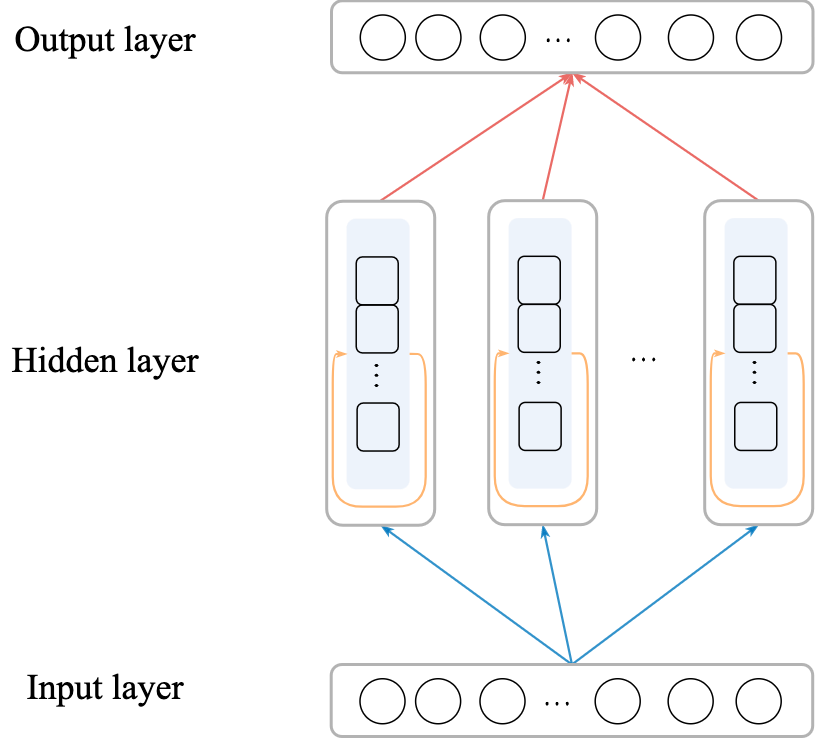
\includegraphics[height=3cm]{float/ch.intro/gesn.png}%
            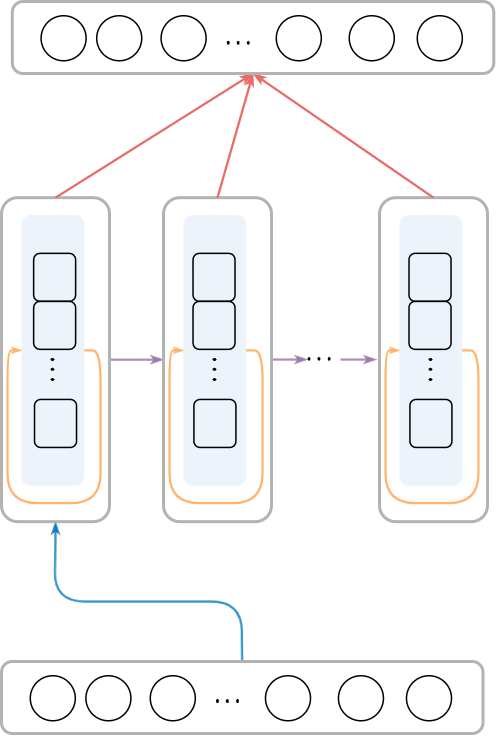
\includegraphics[height=3cm]{float/ch.intro/desn.png}%
        }%
    }
    \setlength{\twosubht}{\ht\twosubbox}    
    \centering
    \subcaptionbox{\label{fig:ch.intro.gesn}GESN结构}{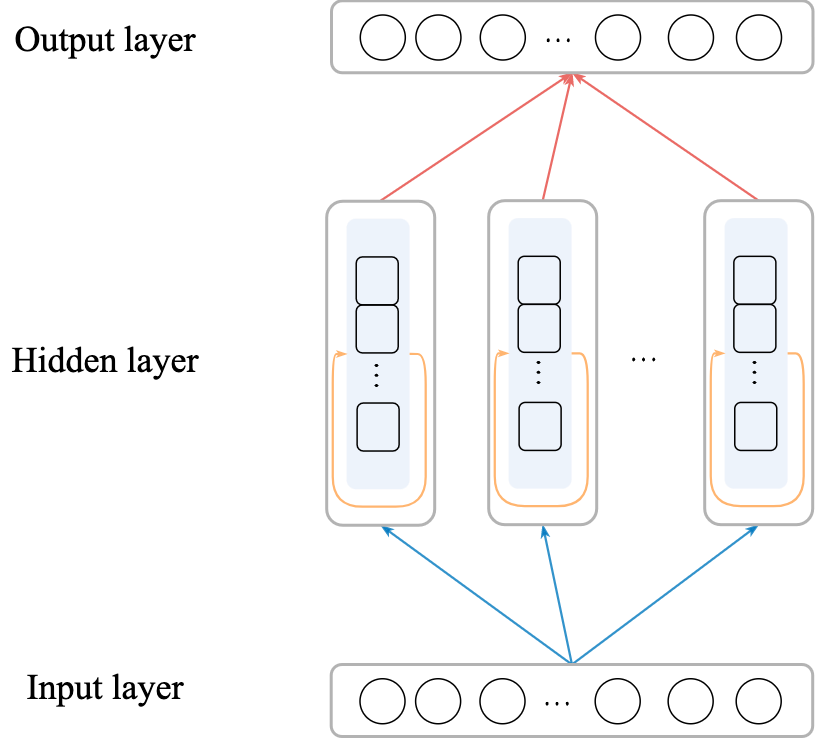
\includegraphics[height = \twosubht]{float/ch.intro/gesn.png}}
    \quad
    \subcaptionbox{\label{fig:ch.intro.desn}DESN结构}{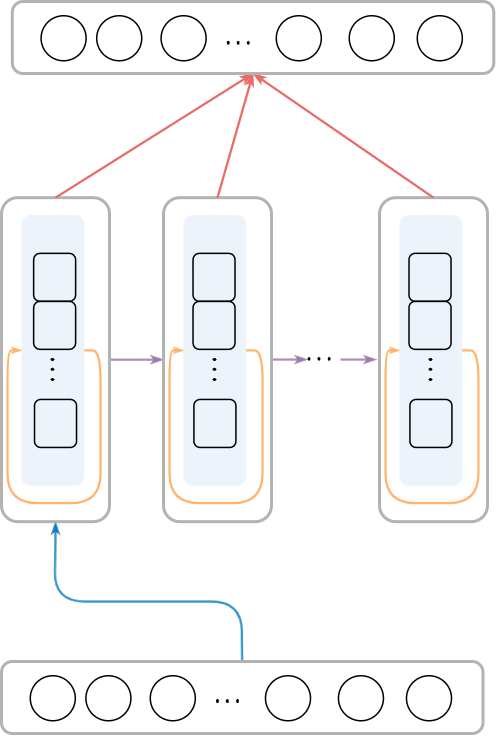
\includegraphics[height = \twosubht]{float/ch.intro/desn.png}}
    \caption{\label{fig:ch.intro.esns} GESN与DESN结构示例}
\end{figure*}

相比循环结构的SDNN预测建模技术研究,基于卷积结构的SDNN预测建模研究则更为薄弱 。He et al.~\cite{hePowerful2016}首先发现了基于随机卷积核的VGG构型\footnote{{https://www.robots.ox.ac.uk/~vgg/research/very\_deep/}}~\cite{simonyanVery2015}CNN在纹理生成(Texture synthesis)和风格迁移(Style transfer)等任务上具有不亚于梯度下降训练CNN的表现。受此启发,Antognini et al.~\cite{antogniniAudio2019}发现了基于一维卷积结构的随机CNN模型在音频纹理生成任务上同样可以达到与训练CNN一样的性能。进一步地,Yu et al.~\cite{yuImpact2019}在合成时间序列数据集和煤气供应数据集等现实时间序列数据集上进行了一维随机CNN的预测建模实验,展示了随机映射方法在CNN预测建模技术中的可行性。

由此,针对时间序列深度学习预测技术模型选择挑战中的低效问题,构造基于随机映射的深度学习预测建模技术是一种有效的解决途径,既可以兼具深度学习建模技术优异的预测潜能,又可以利用随机映射技术收敛快、效率高的优势,从而高效灵活的解决深度学习预测建模技术的模型选择效率问题,为时间序列深度学习预测建模技术的实际应用和发展提供支撑。

然而,基于随机映射方法的预测建模研究,尤其是SDNN预测建模研究,仍有一些突出的问题和限制。这些问题对于不同的神经网络结构,如卷积结构和循环结构,呈现出不同的复杂表现。
例如,相较于梯度下降方法,随机映射方法在提升模型建模效率的同时,因其输入层和隐藏层权重参数的随机性,不可避免地在一定程度上降低了模型的预测性能,这种现象对于具备复杂表征结构的卷积结构SDNN预测模型而言尤为突出,如何设计一种卷积结构SDNN预测模型构造与选择方法以保持模型建模效率与预测性能的平衡性是基于卷积结构的SDNN预测建模技术研究中的重要问题。

又如,现有循环结构SDNN预测模型(即ESN预测模型)的研究主要集中于隐藏神经网络结构的设计与优化\cite{liPSObased2019,chouikhiPSObased2017},而输出结构选择问题尚未有关注。在ESN预测模型的输出结构设计中,存在诸多问题,如基于梯度下降方法所构造的RNN模型输出结构是否适用于随机映射方法下的循环结构建模技术和方法,这些输出结构对于ESN模型输出结构的优化有何启示,如何选择与优化ESN预测模型的循环输出结构等。这些问题是基于循环结构的SDNN预测建模技术研究中的重要问题,需要进一步研究和探索。

再者,时间序列输入特征的选择问题是以CNN与RNN为代表的不同结构DNN预测建模技术共性问题,如何将深度神经网络结构与时间序列输入特征有效结合,从而建立兼容不同结构SDNN预测模型的特征选择方法,是进一步系统提升SDNN预测模型性能的关键。

此外,基于不同结构的SDNN预测建模有着不同的特性和适用场景。单一特定结构下的SDNN预测建模与优化方法难以适应复杂多变的现实时间序列预测需要。如何集成多种深度神经网络结构的优势,针对不同的时间序列预测建模场景,自适应地选择合适的神经网络结构及其参数,从而建立SDNN预测模型混合结构下的构造与优化技术,亦是基于随机映射的深度学习预测建模技术研究及其应用中的关键问题。

因此,为解决现有深度学习预测建模技术与随机映射方法的不足,本文将在时间序列深度学习预测建模技术与随机映射方法相关研究的基础上,尝试设计SDNN预测模型的新颖构造方法,以消除传统迭代训练的DNN预测模型所带来的低效性问题和随机映射方法在DNN网络结构上的不稳定性,同时建立与预测问题和预测模型相适应的模型选择算法,
探索具备高效自适性、理论创新性和良好应用性的SDNN时间序列建模技术。
本研究在一定程度上推动深度学习预测模型理论发展,充分挖掘随机映射方法在时间序列深度学习预测建模技术中的性能潜力,具有一定的理论创新意义和良好的现实应用意义。

% \chapter[误差反馈随机映射卷积神经网络预测模型构造方法]{误差反馈随机映射卷积神经网络预测模型构造方法
% \footnote[11]{本章主要内容已发表在:Zhang, Xinze, Kun He, and Yukun Bao. "Error-feedback stochastic modeling strategy for time series forecasting wi th convolutional neural networks." Neurocomputing 459 (2021): 234-248.}
% }

\chapter{基于卷积结构的SDNN预测模型构造与优化方法 \label{sec:chapter.cnn}
% \footnote[11]{本章主要内容已发表在:Zhang, Xinze, Kun He, and Yukun Bao. "Error-feedback stochastic modeling strategy for time series forecasting wi th convolutional neural networks." Neurocomputing 459 (2021): 234-248.}
}


\section{引言}
% 基于深度学习的时间序列预测建模技术在众多现实决策问题中发挥了重要作用。
% 发明准确高效的时间序列预测建模技术具有重要的理论意义和现实应用价值。
近年来,作为深度神经网络(DNN)的代表结构之一,基于卷积结构的卷积神经网络(CNN)因其优异的特征提取能力与学习能力已被广泛地应用于时间序列预测建模问题中~\cite{sezer2018algorithmic,cavalliCNNbased2021,sadaei2019short}。
然而,如何基于时间序列数据自适应地选择模型结构与参数是应用CNN预测建模技术中的关键挑战。
对于模型选择问题,已有众多研究者展开了相关研究。
Elsken et al.~\cite{elskenNeural2019a}对神经网络模型的既有模型选择方法进行了研究综述,总结出定义神经网络参数搜索空间、针对参数训练模型和基于训练模型结构对所搜索参数加以优化的模型选择范式。
但是,这种传统的模型选择范式需要消耗大量的计算资源与训练时间,使得卷积神经网络时间序列预测建模技术的现实应用面临参数构造难、计算开销大等阻碍~\cite{zela2018towards}。

相较于有训练权重参数的CNN模型,采用随机映射方法构造的CNN模型在图像风格迁移、语音合成、函数拟合等问题中展现出充分潜力~\cite{hePowerful2016,antogniniAudio2019,yuImpact2019}。
这种基于随机映射的CNN模型具有计算开销低、收敛速度快、学习性能好等特点,但也存在网络结构设计难、随机权重输出结果不稳定等问题。
针对时间序列预测问题,Yu et al.~\cite{yuImpact2019}通过将CNN模型中的卷积权重随机初始化并固定,利用最小二乘法闭式求解输出权重,建立了随机卷积神经网络预测模型,并结合合成时间序列数据和煤气供应数据,验证了其方法的可行性。
但此预测建模方法存在若干问题。首先,其卷积结构的选择依赖于人工经验,使得模型无法根据不同预测情景自适应选择合适参数;其次,输出权重全局更新的求解方式,随着卷积核数量的增加,将使卷积层的隐藏特征维度倍数增加,导致求解输出权重的最小二乘法出现病态矩阵问题,削弱了模型的稳定性,甚至使模型出现欠拟合的问题。
因此,如何建立基于卷积结构的随机深度神经网络(SDNN)预测模型的新颖构造及自适应优化方法,解决已有卷积结构SDNN预测建模技术中参数选择时的人工依赖、输出权重求解时的病态矩阵和预测过程的不稳定性,以有效利用随机映射方法的效率优势与卷积结构的学习能力,是本章的研究重点。

为此,本章在已有研究的基础上,针对基于卷积结构的SDNN预测模型构造与自适应优化问题,创新地提出了一种基于误差反馈随机建模(Error-feedback stochastic modeling, ESM)和贪心搜索选择的CNN构造与优化方法(ESM-CNN)。在ESM-CNN这一卷积结构的SDNN预测模型构造与优化方法中,ESM策略通过递归生成随机映射卷积核的方式提高了模型构造效率,并借助误差反馈策略,单独求解各卷积核输出权重,保证了所构造模型的理论收敛性,以此高效构造出具有理论收敛性的预测模型;同时,通过贪心算法解决模型构造中随机映射卷积核的选择问题,使得ESM-CNN能够自适应的在单卷积层内具备不同卷积宽度的卷积核,以此增强了ESM-CNN学习不同尺度时间序列特征的能力,进一步地提高了模型预测性能;最后,采用合成数据和多个真实数据集充分验证了ESM-CNN的有效性以及卷积核选择方法的必要性,与传统随机多层感知机(SMLP)模型和梯度下降训练DNN模型相比,ESM-CNN具有优秀的预测性能与建模效率,是解决时间序列预测问题的有效方法。



本章的主要内容包括:\secref{sec:esm.cnn}简要介绍了传统CNN预测模型的构造过程,并对本章节所提出的ESM-CNN模型构造与优化方法进行了详细阐述;\secref{sec:esm.exp}从数据集选取、对比模型选取、评价指标选取、实验流程和实验环境等方面介绍了本章的实验方案;\secref{sec:esm.ana}比较、分析和总结了各模型在所选数据集上的实验结果;最后,\secref{sec:esm.conc}对本章予以小结。

\section{ESM-CNN预测模型 \label{sec:esm.cnn}}

\subsection{CNN预测模型}
卷积神经网络(CNN)是将输入连接卷积核做局部非线性变换,并池化展开特征图所构成的神经网络~\cite{lecun1995convolutional}。
卷积是指输入的滑动局部非线性变换。
通过对时间序列输入特征的卷积操作,卷积核(Convolutional filter)能够基于完整输入学习出有用的非线性特征,并建立起所学习特征与对应卷积核宽度(Filter size)输入的关系,由此组成了卷积层(Convolutional layer)的输出特征图(Feature map)。这些特征图往往被送入池化层(Pooling layer)进行下采样(Subsample)以降低卷积层的输出带宽(Output band),同时增强神经网络对异常特征图值的鲁棒性~\cite{yang2015deep,zhao2017convolutional,koprinskaConvolutional2018}。
池化操作后的特征图会继续送入神经网络的下一层结构中,以学习更抽象的表示或生成输出结果。

这里,本节对一种典型结构CNN预测模型进行具体介绍,该模型由生成特征图的单卷积层、进行下采样的平均池化层(Pooling layer)和生成预测结果的全连接层(Fully connected layer)组成。
对于由$N$个样本组成的时间序列数据$D=\left\{\left(X_{i}, Y_{i}\right) \in\left(\mathbb{R}^{T} \times \mathbb{R}^{H}\right)\right\}_{i=1}^{N}$,其中$X_i$表示历史T步内的时间序列观测值$X_i = [x_1,\dots, x_T]^{\trans}$,$Y_i$表示预测时长H步内的时间序列观测值$Y_i = [x_{T+1},\dots, x_{T+H}]^{\trans}$。一个具有$C$个卷积核的CNN预测模型可表示为如\autoref{eq:conv},\autoref{eq:pool}和\autoref{eq:sec.cnn.fc}所示过程:
\begin{align}
    m_j^t &= \sigma \left(\sum^{K_m}_{k_m=1} w^{k_m}_j x_{t+k_m-1} +b_j\right), \quad &t &= 1,\dots, T-K_m +1, \label{eq:conv}  \\
    p_j^i &= \frac{\sum^{K_p}_{k_p=1} m_j^{i+k_p-1}}{K_p}, \quad &i &= 1,..., T-K_p - K_m+2, \label{eq:pool} \\
    f_C &= \sum^C_{j=1} \left( \sum^{T-K+2}_{i=1}\beta_{j}^i p_j^i\right) + \beta_0.& & \label{eq:sec.cnn.fc}
\end{align}

\autoref{eq:sec.cnn.fc}中,$K = K_p + K_m$,$K_p$和$K_m$分别为池化操作与卷积操作的宽度大小。
\autoref{eq:pool}中,${m}_j$为特征图向量$[m_j^1, \ldots, m^{T-{K_m}+1}_j]^{\mathrm{T}}$,基于第$j$个卷积在输入时间序列做如\autoref{eq:conv}所示的卷积操作后得到。
$\sigma(\cdot)$表示卷积核所使用的激活函数。在本章节中,$\sigma(\cdot)$为sigmoid激活函数。
${w_j} = [w_j^1,\ldots, w_j^{K_m}]$和$b_j$分别为第$j$个卷积核的权重与偏置项。
$p_j$表示对${m}_j$做如\autoref{eq:pool}所示平均池化操作后的池化特征图向量$[p_j^1, \ldots, p^{T-{K}+2}_j]^{\mathrm{T}}$。
$[\beta_1^1, \beta_1^2,\ldots,\beta_C^{T-K+2}]$和$\beta_0$为第$j$个卷积核与输出层间的全连接层权重与偏置项,$\beta_j^i = [\beta_{j}^{i,1},\ldots,\beta_{j}^{i,H}]^{\mathrm{T}}$。

\begin{figure*}[!t]
    \centering
    \includegraphics[width = \textwidth]{float/ch.cnn/esm-cnn.png}
    \caption{\label{fig:esm_arch} ESM-CNN预测模型神经网络结构}
\end{figure*}

在传统的CNN预测模型构造方法中,通过以减小预测误差$\| e \|$为目标,梯度下降训练包含所有权重项与偏置项在内的权重参数,CNN能够有效学习出历史输入时间序列与预测目标时间序列间的函数关系,生成良好的预测结果。
但这种构造方法需要预先定义包含卷积核宽度、卷积核数量、梯度下降学习速率等众多超参数(Hyper-parameters),进过反复迭代训练评价后,才能选择出合适的超参与权重参数组合。此过程往往会消耗大量的计算资源和时间,存在显著的改进空间。


为解决现有CNN预测建模技术模型选择困难、计算开销高等问题,本章提出了一种误差反馈随机建模(ESM)构造策略,结合基于贪心算法的卷积核选择算法,建立ESM-CNN预测模型。该模型神经网络结构如\autoref{fig:esm_arch}所示,其中绿色线、黄色线和蓝色线分别表示不同结构随机卷积核的卷积与池化操作,深浅不同的红色线表示迭代局部更新的输出权重,同一深度的红色线表示链接同一卷积核的输出权重。

\subsection{误差反馈随机建模策略\label{sec:esm.esm}}
为高效构造具备可靠预测性能的卷积结构SDNN预测模型,利用随机映射方法的优异建模效率,同时解决随机映射算法对预测性能稳定性的干扰,本节提出了一种ESM策略,建立CNN构型下的SDNN预测模型。
该方法通过在单卷积层内递归增长添加固定随机初始化权重卷积核的方式构造CNN隐藏结构,同时利用误差反馈闭式计算新增卷积核所对应的输出权重参数,以此完成整个预测模型的构造过程,同时为模型的预测函数拟合能力提供理论收敛保证。

具体地,对于一个已具有$C$个卷积核的单卷积层ESM-CNN,其模型可被公式表述为:
\begin{equation}
    \label{eq:sccnn}
    f_C = \sum^C_{j=1} \left( \sum^{T-K+2}_{i=1}\beta_{j}^i p_j^i + \beta^0_j \right),
\end{equation}
并进一步简写为:$f_C= \sum^C_{j=1}\sum^{T-K+2}_{i=0} \beta_j^i p_j^i$。



\autoref{eq:sccnn}中,$\beta_j = [\beta_j^0, \beta_j^1, \ldots, \beta_j^{T-K+2}]$ 表示全连接输出层中连接第$j$个卷积核池化特征图向量与输出单元的权重参数,$p_j^0 = I$。
ESM-CNN的预测误差如\autoref{eq:sec.cnn.error}所示:
\begin{equation}
    e_C = Y- f_C = [e_C^1,\ldots, e_C^H]. \label{eq:sec.cnn.error}
\end{equation}

若预测模型的均方误差(Mean square error,MSE)未降低至容忍水平$\varrho$,ESM策略将继续新增一个随机映射卷积核$m_{C+1}$生成对应的池化特征图向量$p_{C+1}$,并将$p_{C+1}$全连接至输出层中以加宽模型隐藏结构。
其中,新增卷积核所对应的全连接输出层权重将基于当前模型的预测误差$e_C$反馈,通过如\autoref{eq:scupdate}最小二乘法加以求解:
\begin{equation}\label{eq:scupdate}
    \left[\beta_{{C+1}}^0, \ldots, \beta_{{C+1}}^{T-K+2} \right]=\argmin _{\beta}\|e_C -\sum_{i=0}^{T-K+2} \beta_{C+1}^i p_{C+1}^i \|.
\end{equation}

通过此策略,所构造的ESM-CNN预测模型能够具备随着卷积核数量增加而单调下降并收敛的预测误差,从而完成对预测目标函数的逼近。该性质通过如下代数推导予以证明:
\begin{proof}

    定义ESM-CNN的预测误差中间项为:$\tilde{e}_{C+1}^{\, 0}, \ldots, \tilde{e}_{C+1}^{\, T-K+2} $,新增卷积核所对应的全连接输出层权重中间项为:$\tilde{\beta}_{C+1}^{\, 0}, \ldots, \tilde{\beta}_{C+1}^{\, T-K+2}$,中间项之间的计算关系为:
    \begin{alignat*}{2}
        & \tilde{e}_{C+1}^{\, i+1}       & = & \mspace{18mu} \tilde{e}_{C+1}^{\, i}-\tilde{\beta}_{C+1}^{\, i+1} p_{C+1}^{i+1}, \quad i = 0,\ldots,T-K+1,                                        \\
       \shortintertext{其中,}
        & \tilde{\beta}_{C+1}^{\, i+1}   & = & \mspace{18mu} [\tilde{\beta}_{C+1}^{\, i+1,1}, \ldots,\tilde{\beta}_{C+1}^{\, i+1,h},\ldots, \tilde{\beta}_{C+1}^{\, i+1,H}],                     \\
        & \tilde{\beta}_{C+1}^{\, i+1,h} & = & \mspace{18mu} \left\langle \tilde{e}_{C+1}^{\, i,h}, p_{C+1}^{\, i+1}\right\rangle /\left\|p_{C+1}^{\, i+1}\right\|^{2} , \quad h= 1, \ldots, H , \\
       \shortintertext{同时,}
        & \tilde{e}_{C+1}^{\, 0}         & = & \mspace{18mu} e_{C}- \tilde{\beta}_{C+1}^{\, 0} p_{C+1}^{\, 0},                                                                                   \\
        & \tilde{\beta}_{C+1}^{\, 0}   & = & \mspace{18mu} [\tilde{\beta}_{C+1}^{\, 0,1}, \ldots,\tilde{\beta}_{C+1}^{\, 0,h},\ldots, \tilde{\beta}_{C+1}^{\, 0,H}],                     \\
        & \tilde{\beta}_{C+1}^{\, 0,h} & = & \mspace{18mu} \left\langle {e}_{C}^{\, h}, p_{C+1}^{\, 0}\right\rangle /\left\|p_{C+1}^{\, 0}\right\|^{2} , \quad h= 1, \ldots, H , \\
        % \shortintertext{可得:}
        & \tilde{e}_{C+1}^{\, T-K+2} \,  & = & \mspace{18mu} {e}_{C} - \sum^{T-K+2}_{i=0} \tilde{\beta}_{C+1}^{\, i} p_{C+1}^{\, i}.
   \end{alignat*}
因新增卷积核所对应的全连接输出层权重基于最小二乘法予以求解:
$$
\left[\beta_{{C+1}}^0, \ldots, \beta_{{C+1}}^{T-K+2} \right]=\argmin _{\beta} \,\|e_C -\sum_{i=0}^{T-K+2} \beta_{C+1}^i p_{C+1}^i \|,
$$
则$\left\|e_{C+1}\right\|^{2}$与$\left\|\tilde{e}_{C+1}^{\, T-K+2}\right\|^{2}$存有不等式关系:
$$
    \|e_{C+1}\|^{2} \,= \min _{\beta} \,\| e_C -\sum_{i=0}^{T-K+2} {\beta}_{{C+1}}^i p_{C+1}^i \|^{2}  \, \leq  \| {e}_{C} - \sum^{T-K+2}_{i=0} \tilde{\beta}_{C+1}^{\, i} p_{C+1}^{\, i} \|^{2} \, =  \|\tilde{e}_{C+1}^{\, T-K+2}\|^{2}.
$$
同时,预测误差中间项之前存在着单调下降性质:
\begin{align*}
    & \|\tilde{e}_{C+1}^{\, i+1}\|^2-\|\tilde{e}_{C+1}^{\, i}\|^2 \\
    ={}    & \sum_{h=1}^{H}
    \left(
    \langle \tilde{e}_{C+1}^{\, i,h}-\tilde{\beta}_{C+1}^{\, i+1,h} p_{C+1}^{i+1}
    ,
    \tilde{e}_{C+1}^{\, i,h}-\tilde{\beta}_{C+1}^{\, i+1,h} p_{C+1}^{i+1} \rangle
    -
    \langle \tilde{e}_{C+1}^{\, i,h}, \tilde{e}_{C+1}^{\, i,h} \rangle
    \right)                                                              \\
    ={}    & \sum_{h=1}^{H}
    \left(
    \langle \tilde{\beta}_{C+1}^{\, i+1} p_{C+1}^{i+1}
    ,
    \tilde{\beta}_{C+1}^{\, i+1} p_{C+1}^{i+1} \rangle
    -
    2 \langle \tilde{e}_{C+1}^{\, i,h} , \tilde{\beta}_{C+1}^{\, i+1} p_{C+1}^{i+1} \rangle
    \right)                                                              
    \\
    ={}    & \sum_{h=1}^{H}
    \left(
    \langle 
    \frac{\left\langle \tilde{e}_{C+1}^{\, i,h}, p_{C+1}^{\, i+1}\right\rangle}{\left\|p_{C+1}^{\, i+1}\right\|^{2}}  
    p_{C+1}^{i+1}
    ,
    \frac{\left\langle \tilde{e}_{C+1}^{\, i,h}, p_{C+1}^{\, i+1}\right\rangle}{\left\|p_{C+1}^{\, i+1}\right\|^{2}}  
    p_{C+1}^{i+1}
    \rangle
    -
    2 
    \langle 
    \tilde{e}_{C+1}^{\, i,h} 
    ,
    \frac{\left\langle \tilde{e}_{C+1}^{\, i,h}, p_{C+1}^{\, i+1}\right\rangle}{\left\|p_{C+1}^{\, i+1}\right\|^{2}}  
    p_{C+1}^{i+1} 
    \rangle
    \right)                                                              
    \\
    ={}    & \sum_{h=1}^{H}
    \left(
    \frac{{\left\langle \tilde{e}_{C+1}^{\, i,h}, p_{C+1}^{\, i+1}\right\rangle}^2}{\left\|p_{C+1}^{\, i+1}\right\|^{4}}  
    \langle 
    p_{C+1}^{i+1}
    ,
    p_{C+1}^{i+1}
    \rangle
    -
    2 \frac{\left\langle \tilde{e}_{C+1}^{\, i,h}, p_{C+1}^{\, i+1}\right\rangle}{\left\|p_{C+1}^{\, i+1}\right\|^{2}}  
    \langle \tilde{e}_{C+1}^{\, i,h} 
    ,
    p_{C+1}^{i+1} 
    \rangle
    \right)                                                              
    \\
    ={}    & \sum_{h=1}^{H}
    \left(
    \frac{{\left\langle \tilde{e}_{C+1}^{\, i,h}, p_{C+1}^{\, i+1}\right\rangle}^2}{\left\|p_{C+1}^{\, i+1}\right\|^{4}}  
    {\left\|p_{C+1}^{\, i+1}\right\|^{2}}  
    -
    2 \frac{{\left\langle \tilde{e}_{C+1}^{\, i,h}, p_{C+1}^{\, i+1}\right\rangle}^2}{\left\|p_{C+1}^{\, i+1}\right\|^{2}}  
    \right)                                                              
    \\        
    ={}    & \sum_{h=1}^{H}
    \left(
    - {\langle \tilde{e}_{C+1}^{\, i,h}, p_{C+1}^{\, i+1} \rangle}^2 / \left\|p_{C+1}^{\, i+1}\right\|^{2}
    \right)                                                              \\
    \leq{} & 0 .
    \end{align*}
该性质在$\left\|\tilde{e}_{C+1}^{\, 0}\right\|^{2}$与$\left\|e_{C}\right\|^{2}$间仍然保持:
\begin{align*}
    & \|\tilde{e}_{C+1}^{\,0}\|^2-\|{e}_{C}\|^2 \\
    ={}    & \sum_{h=1}^{H}
    \left(
    \langle {e}_{C}^{\, h}-\tilde{\beta}_{C+1}^{\, 0,h} p_{C+1}^{0}
    ,
    {e}_{C}^{\, h}-\tilde{\beta}_{C+1}^{\, 0,h} p_{C+1}^{0} \rangle
    -
    \langle {e}_{C}^{\, h}, {e}_{C}^{\, h} \rangle
    \right)                                                              \\
    ={}    & \sum_{h=1}^{H}
    \left(
    \langle \tilde{\beta}_{C+1}^{\, 0,h} p_{C+1}^{0}
    ,
    \tilde{\beta}_{C+1}^{\, 0,h} p_{C+1}^{0} \rangle
    -
    2 \langle {e}_{C}^{\, h} , \tilde{\beta}_{C+1}^{\, 0,h} p_{C+1}^{0} \rangle
    \right)                                                              
    \\
    ={}    & \sum_{h=1}^{H}
    \left(
    \langle 
    \frac{\left\langle {e}_{C}^{\, h}, p_{C+1}^{\, 0}\right\rangle}{\left\|p_{C+1}^{\, 0}\right\|^{2}}  
    p_{C+1}^{0}
    ,
    \frac{\left\langle {e}_{C}^{\, h}, p_{C+1}^{\, 0}\right\rangle}{\left\|p_{C+1}^{\, 0}\right\|^{2}}  
    p_{C+1}^{0}
    \rangle
    -
    2 
    \langle 
    {e}_{C}^{\, h} 
    ,
    \frac{\left\langle {e}_{C}^{\, h}, p_{C+1}^{\, 0}\right\rangle}{\left\|p_{C+1}^{\, 0}\right\|^{2}}  
    p_{C+1}^{0} 
    \rangle
    \right)                                                              
    \\
    ={}    & \sum_{h=1}^{H}
    \left(
    \frac{{\left\langle {e}_{C}^{\, h}, p_{C+1}^{\, 0}\right\rangle}^2}{\left\|p_{C+1}^{\, 0}\right\|^{4}}  
    \langle 
    p_{C+1}^{0}
    ,
    p_{C+1}^{0}
    \rangle
    -
    2 \frac{\left\langle {e}_{C}^{\, h}, p_{C+1}^{\, 0}\right\rangle}{\left\|p_{C+1}^{\, 0}\right\|^{2}}  
    \langle {e}_{C}^{\, h} 
    ,
    p_{C+1}^{0} 
    \rangle
    \right)                                                              
    \\
    ={}    & \sum_{h=1}^{H}
    \left(
    \frac{{\left\langle {e}_{C}^{\, h}, p_{C+1}^{\, 0}\right\rangle}^2}{\left\|p_{C+1}^{\, 0}\right\|^{4}}  
    {\left\|p_{C+1}^{\, 0}\right\|^{2}}  
    -
    2 \frac{{\left\langle {e}_{C}^{\, h}, p_{C+1}^{\, 0}\right\rangle}^2}{\left\|p_{C+1}^{\, 0}\right\|^{2}}  
    \right)                                                              
    \\        
    ={}    & \sum_{h=1}^{H}
    \left(
    - {\langle {e}_{C}^{\, h}, p_{C+1}^{\, 0} \rangle}^2 / \left\|p_{C+1}^{\, 0}\right\|^{2}
    \right)                                                              \\
    \leq{} & 0 .
    \end{align*}
因此,ESM-CNN的预测误差收敛性可证:
$$
\|e_{C+1}\|^2  \; \leq \|\tilde{e}_{C+1}^{\, T-K+2}\|^2 \; \leq \|\tilde{e}_{C+1}^{\,0}\|^2 \; \leq \|{e}_{C}\|^2 .
$$
\NoEndMark
\end{proof}

与全局更新输出层权重的构造方式不同,本章所提出的ESM构造策略通过误差反馈迭代局部更新输出层权重的方式完成输出层权重的计算。具体地,ESM构造策略具备以下三种优势:1)与全局更新输出层权重相比,迭代局部更新输出层权重的方式具有更小的计算开销,这种低开销优势会随隐藏层结构的增大同时扩大;2)随着卷积层中递归新增卷积核的不断加入,链接至输出层的池化特征图向量维度会同时倍数增大,与预测目标维度相比过大的特征维度会导致闭式求解算法的病态问题(Ill-posed problem)\cite{vogel2002computational},进而破坏预测性能的稳定性和鲁棒性;3)基于误差反馈递归更新输出权重构造的预测模型能在神经网络隐藏构造的过程中不断弥补上步预测误差,同时,这种历史输出权重保持固定的方式在一定程度上承担了正则化的作用,从而增强了所构造模型的性能稳定性。

\subsection{卷积参数贪心选择方法
\label{sec:chapCNN.greedy}}
针对ESM-CNN预测模型构造过程中的卷积核选择问题,本章节提出了一种基于贪心算法的卷积核选择方法,使得ESM-CNN具有在单卷积层中同时具备不同宽度的卷积核结构,以此增强模型对于不同尺度时间序列特征的学习建模能力。

对于如\autoref{eq:sccnn}所示具有$C$个卷积核的单卷积层ESM-CNN,在新增卷积核结构时,基于均匀分布(Uniform distribution)$[-\lambda, \lambda]$、卷积与池化宽度$\{(K_{m,s}, K_{p,s})\}^S_{s=1}$生成一批对应的池化特征图向量 $\{p_{{C+1},s} \}^S_{s=1}$表示对应的备选卷积核结构。
为评价这些备选卷积核结构,利用将备选卷积核加入当前网络中所能下降的预测误差,本节提出了一种卷积核评分$\Delta_{{C+1, s}}$,其计算方式如\autoref{eq:filterScore}所示:
\begin{align}
    \Delta_{{C+1},s} & = \| e_{C+1,s} \|^2 - \| e_{C} \|^2 \label{eq:filterScore}                                                                      \\
    {}               & = \|\ e_C -\sum_{i=0}^{T-K^{\prime}+2} \beta_{C+1, s}^i p_{C+1, s}^i \|^2 -  \| e_{C} \|^2, \notag  
\end{align}

\autoref{eq:filterScore}中,$K^{\prime} = K_{m,s} + K_{p,s}$,$p^i_{C+1, s}$和$\beta^i_{C+1, s}$分别由\autoref{eq:pool}和\autoref{eq:scupdate}计算得出。
基于所提出的卷积核评分$\Delta_{{C+1, s}}$,将实现最好预测效果提升的备选卷积核$p_{C+1}^{*}$选出,作为新增卷积核正式加入当前神经网络结构,该过程如\autoref{eq:scselection}所示:
\begin{equation}\label{eq:scselection}
    p_{C+1}^{*} = \argmax\limits_{p_{{C+1},s}} \{ \Delta_{{C+1},s}, s = 1,\ldots,S \}.
\end{equation}

在此之后,新增卷积核所对应的全连接输出层权重通过\ref{eq:scupdate}求解得出。结合本章节所提出的ESM构造策略与卷积核选择方法,高效构造出一种具备多尺度时间序列特征学习能力、预测函数拟合收敛性和稳定预测性能的ESM-CNN预测模型。
% \autoref{fig:esm_arch}详细描绘了ESM-CMM预测模型的神经网络结构。

\begin{figure*}[!t]
    \centering
    \includegraphics[width = 0.8\textwidth]{float/ch.cnn/flow.png}
    \caption{\label{fig:flowchart} ESM-CNN预测模型构造过程}
\end{figure*}

\subsection{ESM-CNN构造过程}
如\autoref{fig:flowchart}所示,ESM-CNN预测模型的构造过程主要包含:预处理、初始化、评价和更新四个环节。
具体地,所述模型及构造过程为:

(1)对于时间序列数据,构造训练数据集$D=\left\{\left(X_{i}, Y_{i}\right) \in\left(\mathbb{R}^{T} \times \mathbb{R}^{H}\right)\right\}_{i=1}^{N}$,并将数据集$D$归一化至标准正态分布。其中,$N$为数据集$D$中的总样本数,数据集中样本$(X_i,Y_i )$由包含历史T时刻内的时间序列数据$[x_1,\ldots,x_T ]^{\trans}$和未来H步时刻内的时间序列预测目标$[x_{T+1},\ldots,x_{T+H}]^{\trans}$组成。

(2) 设定ESM-CNN预测模型的初始化参数,包括容忍水平$\varrho $,最大特征图通道数$C_{\max}$,初始预测误差$e_0 = [x_{T+1},\ldots,x_{T+H}]^{\trans}$,卷积核宽度$K_m$选择范围$M=\{ K_{m,s}\}^S_{s=1}$与池化操作宽度挑选范围$P=\{K_{p,s}\}^S_{s=1}$,以及卷积核权重的随机初始化分布$[-\lambda,\lambda]$。

(3)在终止条件为特征图通道数$C\leq C_{\max}$或当前模型预测结果的MSE小于$\varrho $的构造过程中,基于卷积核宽度选择范围$M$与池化操作宽度选择范围$P$,依次从参数组合$(K_{m,s}, K_{p,s})$和均匀分布$[-\lambda,\lambda]$中生成$S$个备选卷积核,以此构成卷积核备选集,并根据得到的备选集,计算各备选卷积核下的池化特征图向量$\{ p_{C+1,s}\}^S_{s=1}$。

(4)基于\autoref{eq:filterScore}计算各备选卷积核的评分,从中贪心选出最优的卷积核结构及对应卷积核权重,将其加入当前神经网络结构中,更新卷积层卷积核数量和模型预测误差。迭代此过程,直至满足终止条件。


\section{实验设计与流程\label{sec:esm.exp}}
\subsection{数据集描述}
为充分评估所提ESM-CNN预测模型的预测性能和验证其收敛能力,本章节在经典人工合成时间序列数据集和多项真实时间序列数据集上进行实验验证研究。实验数据集名称及简写如\autoref{tab:cnn.dataName}所示。
\autoref{tab:app_data}展示了本章节所用数据集的统计信息。其中,第一列、第五列和第六列说明了所用数据集的名称,起始截止日期和大小。
第二列展示所用数据集的平稳性(Stationarity)状态,“\cmark”表示该数据集为平稳的,“\xmark'表示该数据集为非平稳的,该状态通过扩张的迪基-福勒检验(Augmented Dickey Fuller,ADF)\footnote{https://www.statsmodels.org/stable/generated/statsmodels.tsa.stattools.adfuller.html}判断得出。第三列与第四列则分别表示了数据集的趋势性(Trend)与季节性(Seasonality)强度分数\footnote{https://otexts.com/fpp2/seasonal-strength.html},分数越高表明该数据具备越强的趋势性或季节性。各数据集的说明如下:

\begin{table}[!t]
    \centering
    \caption{实验数据集名称及英文缩写对照 \label{tab:cnn.dataName}}
    \begin{tabularx}{\textwidth}{lXl}
        \toprule
        {数据集中文名称} & {数据集英文名称} & 英文缩写 \\  \midrule
        一阶自回归 & First order autoregression & AR1 \\
        比特币两小时美元价格  & Two-hourly bitcoin to U.S. dollar price & BTC          \\
        流感阳性样本率     & Influenza-like illness rate                & ILI          \\
        欧洲布伦特原油周价格  & Weekly Europe Brent crude oil price     & BRENT-weekly \\
        欧洲布伦特原油周价格  & Daily Europe Brent crude oil price      & BRENT-daily  \\
        美国WTI原油周间价格 & Weekly WTI crude oil price              & WTI-weekly   \\
        标普500每日收盘指数 & Daily close value of S\&P 500 index     & S\&P 500     \\
        纳斯达克每日收盘指数  & Daily close value of NASDAQ Composite   & NASDAQ       \\
        道琼斯每日收盘指数   & Daily close value of Dow Jones Average  & DJI          \\
        纽约证交所每日收盘指数 & Daily close value of NYSE Composite     & NYSE         \\
        \bottomrule
        
    \end{tabularx}

\end{table}


\input{float/ch.cnn/data.tex}


针对合成数据上的预测实验研究,AR1数据集作为评价时间序列预测模型的常用基准数据集之一,参照相关研究\cite{qi2008trend,crone2016feature}的参数设定通过\autoref{eq:ar}予以合成:
    \begin{equation}
        \label{eq:ar}
            x_t = \alpha + x_{t-1} + \varepsilon_t,
        %\vspace{-0.1em}    
    \end{equation}
    其中,$\alpha = 0.01$, $\varepsilon_t \sim i.i.d.~\mathrm{U}(-0.25,0.25)$,共合成出500个观测点。

针对比特币价格预测应用研究,本章节所用BTC数据集通过Tradeviw平台\footnote{https://www.tradingview.com/symbols/BTCUSD}采集2020年5月25日至2021年3月20日间的两小时级美元收盘价得到,共有2181个观测点。

针对流感阳性样本率预测应用研究,本章节所用ILI数据集通过中国国家流感中心平台\footnote{https://ivdc.chinacdc.cn/cnic/en/Surveillance/WeeklyReport/} 采集2010年1月15日至2020年4月15日间的中国南方地区每周流感阳性样本率得到,共有535个观测点。

针对原油价格预测应用研究,本章节分别通过采集欧洲BRENT市场\footnote{https://www.eia.gov/dnav/pet/hist/RBRTEd.htm}和美国WTI市场\footnote{ https://www.eia.gov/dnav/pet/hist/rwtcW.htm}公开至2021年5月3日间的每周美元收盘价格及每日美元收盘价格,得到BRENT-weekly(1773个观测点)、BRENT-daily(8620个观测点)、WTI-weekly(1844个观测点)和WTI-daily(8904个观测点)数据。

针对股票指数预测应用研究,本章节通过UCI机器学习数据集\footnote{https://archive.ics.uci.edu/ml/machine-learning-databases/00554/}得到2009年12月31日至2017年11月15日间的S\&P 500、NASDAQ、DJI和NYSE每日收盘指数,各股票指数数据均有1984个观测点。

在本章节进行的实验中,所选数据集对于训练集、验证集和测试集切分遵循机器学习预测建模研究中常用的0.64、0.16和0.2的比例。为进一步分析和比较所提预测模型在提前单步(One-step-ahead)预测与提前多步( Multi-step-ahead)预测上的性能表现,本章节在各数据集上均进行了不同提前时步的预测建模实验。具体地,AR1数据集上的预测时长H分别为1、3、6,输入步长T为15;BTC数据集上的预测时长H分别为1、3(六小时)、6(半日),输入步长T为24(两日);ILI、BRENT-weekly和WTI-weekly数据集上的预测时长H分别为1、4(一个月)、8(两个月),输入步长T为26(半年); BRENT-daily、WTI-daily、S\&P 500、NASDAQ、DJI和NYSE数据集上的预测时长H分别为1、5(一周)、10(两周),输入步长T为30(六周)。

\subsection{对比模型选择}
% \subsubsection{RVFL, IELM和SCN}
为比较ESM-CNN预测模型与传统统计预测模型的性能差异,将输入时间序列最后时刻观测值作为预测值的Naive预测方法、自回归移动平均(Autoregressive Integrated Moving Average,ARIMA)方法\cite{floresEvolutive2012}和Holt’s Winters季节指数平滑(Holt’s Winters Seasonal Exponential Smoothing,HWSES)方法\cite{chatfieldHoltwinters1978}被选为对照组模型以验证所提模型的性能优势。

为比较ESM-CNN预测模型与经典随机映射预测模型的性能差异,RVFL\cite{igelnik1995stochastic}、ILEM\cite{huang2006universal}和SCN\cite{wang2017stochastic}这三种典型随机多层感知机(SMLP)被选为对照组模型。
RVFL、IELM和SCN的随机映射参数(如随机初始化隐藏层权重的分布参数、容忍水平等)与所提ESM-CNN模型参数保持一致,同时RVFL、IELM和SCN中的隐藏层神经元数量与ESM-CNN中卷积核数量保持一致以更好地控制实验变量。

此外,为比较ESM-CNN预测模型与梯度下降训练方法下DNN预测模型的性能差异,CNN、循环神经网络(Recurrent neural network,RNN)以及结合CNN与RNN优势的卷积循环神经网络(Convolutional recurrent neural network,CRNN)这三种代表性神经网络被加入对照组模型中。具体地,本章节提供了基于一种网格搜索(Grid-search)确定隐藏层卷积核数量的单卷积层CNN(GS-CNN)作为CNN的实现模型。针对RNN结构,本章节复现了Salinas等\cite{salinasDeepAR2020}提出的一种基于自回归长短时记忆(Long short term memory,LSTM)网络结构的RNN预测模型DeepAR,该模型在多项现实预测任务中表现出优异性能。此外,本章节复现了Livieris等\cite{livieris2020cnn}基于CNN与RNN结构提出的卷积长短时记忆(Convolutional long short term memory,CLSTM)网络,作为CRNN结构的有力实现。
GS-CNN,DeepAR,和CLSTM预测模型的超参数(如梯度下降优化算法、学习速率和训练迭代次数等)基于通行的试错(Trial and error)策略予以确定。

进一步地,为验证所提ESM-CNN预测模型中误差反馈构造策略与卷积核结构选择方法的必要性,本章节针对这两个要素进行了消融实验研究。
通过移除卷积核选择方法保留误差反馈随机建模策略,建立一种消融的误差反馈随机卷积神经网络(Error-feedback stochastic convolutional neural network,ES-CNN)。通过完全移除误差反馈策略与卷积核选择方法,构造出Yu et al.\cite{yuImpact2019}所提出的单纯随机卷积神经网络(Stochastic convolutional neural network,Stoc-CNN)。
在本章节所设置的所有预测任务中,ESM-CNN的最大卷积核数量$C_{\max}$设为100以保证模型收敛。基于实验经验,卷积核权重的随机初始化分布$[-\lambda,\lambda]$设为$[-0.5,0.5]$,备选卷积核的宽度选择范围设为$ \{K_{m,s}\} ^S_{s=1} = \{T/3, T/4, T/5, T/6\}$,为简化卷积核结构搜索问题,参考相关研究\cite{zhao2017convolutional},池化操作宽度固定为$K_p=3$。同一宽度的备选卷积核数量为30。
为保证消融实验的公平性,Stoc-CNN、ES-CNN和ESM-CNN的随机设置参数与卷积核数量均保持一致。

\subsection{评价指标设置}
为多角度评价所提模型与进行对照实验研究,本章节选取了包含百分比误差与绝对值误差在内的三种常用预测准确度评价指标\cite{baoPSOMISMO2014,guo2016robust,zhaoDeep2017},分别为:平均绝对百分比误差(Mean absolute percentage error,MAPE),对称平均绝对百分比误差(Symmetric mean absolute percentage error,SMAPE)和根方平均平方误差(Root mean square error,RMSE)。其计算过程分别如\autoref{eq:mape}、\autoref{eq:smape}和\autoref{eq:rmse}所示:
\begin{equation}
	\label{eq:mape}
	MAPE = \frac1N \sideset{}{_{i=1}^N} \sum \abs{\frac{y_{i} - \hat  y_{i}}{y_i}}.
\end{equation}
\begin{equation}
	\label{eq:smape}
	SMAPE = \frac1N \sideset{}{_{i=1}^N} \sum \abs{\frac{y_{i} - \hat  y_{i}}{y_i + \hat  y_{i}}}.
\end{equation}
\begin{equation}
	\label{eq:rmse}
	RMSE = \sqrt{\frac1N \sideset{}{_{i=1}^N} \sum ({y_{i} - \hat  y_{i}})^2 }.
\end{equation}

其中,$y_i$和$\hat y_i$分别表示真实值与预测值。

\subsection{实验步骤}
在本章节的实验验证研究中,所选数据集均首先基于Z-score方法\footnote{https://scikit-learn.org/stable/modules/preprocessing.html\#preprocessing-scaler}归一化至标准正太分布,而后按照0.64,0.16和0.2的比例切分为训练集、验证集和测试集。
所提ESM-CNN及所有对照组和消融模型均通过训练集和验证集进行训练与交叉验证。
在生成预测结果计算评价指标时,预测生成结果均先被还原至原有数值范围,再进行预测准确度计算。

最终,在所有预测任务中,本章节均对每一预测模型建模20次,对20次预测建模结果结合MAPE、SMAPE和RMSE指标计算预测准确度平均值,以综合表现预测模型预测准确性与稳定性。
本章节所有实验均基于CUDA 10.1版本的GPU加速Pytorch框架\cite{paszkePytorch2019}、Ubuntu 20.04系统环境、Intel 8700K CPU和Nvidia GTX 1070 GPU环境进行,以保证计算环境的一致性。本章节的实验设置与算法代码已开源在Github平台\footnote{https://github.com/XinzeZhang/TimeSeriesForecasting-torch},以方便研究者复现和开展相关工作。



\section{实验结果与分析\label{sec:esm.ana}}
\subsection{预测准确度对比与分析}

\cref{tab:app_mape.std,tab:app_smape.std,tab:app_rmse.std}分别展示了ESM-CNN及对照组模型在AR1、BTC和ILI数据集上的MAPE、SMAPE和RMSE平均结果及标准差,以评价不同模型的准确度与稳定性。
在\cref{tab:app_mape.std,tab:app_smape.std,tab:app_rmse.std}中,括号内为模型结果的标准差,越低的标准差表示模型具有越强的预测稳定性。其中,统计模型的0标准差以“-”表示。
每一预测任务中的最优结果通过粗体加星“\(\star\)”的形式进行展示,次优结果通过粗体加以表示。
另外,\cref{tab:app_mape,tab:app_smape,tab:app_rmse}分别展示了ESM-CNN及对照组模型在原油价格与股票指数数据集上的MAPE、SMAPE和RMSE结果,以补充说明所选模型的对比效果。
% \cref{tab:app_mape,tab:app_smape,tab:app_rmse}分别展示了ESM-CNN及对照组模型在原油价格与股票指数数据集上的MAPE、SMAPE和RMSE结果,以补充说明所选模型的对比效果。
\input{float/ch.cnn/std.tex}
\input{float/ch.cnn/mape.tex}
\input{float/ch.cnn/smape.tex}
\input{float/ch.cnn/rmse.tex}

% 在\cref{tab:app_mape.std,tab:app_smape.std,tab:app_rmse.std,tab:app_mape,tab:app_smape,tab:app_rmse}中,
% 第一列为数据集名称,第二列展示了该数据集上不同预测时长H下的预测任务。第三列至最后一列归类展示了统计模型、梯度下降训练模型以及随机映射模型类别下对照模型与所提模型在各预测任务上的平均结果。
% 平均分值结果越低表示模型具有越准确的预测性能。



基于\cref{tab:app_mape.std,tab:app_smape.std,tab:app_rmse.std,tab:app_mape,tab:app_smape,tab:app_rmse}所示的对照组模型结果,可归纳出以下结论:

(1)作为一种新颖的卷积结构SDNN模型,ESM-CNN在本章节选取的人工合成时间序列数据集与真实时间序列数据集上都保持了优秀的预测准确度,展现出ESM-CNN预测模型的良好应用性。

(2)与Naive、ARIMA和HWSES所代表的统计模型相比,ESM-CNN在本章节设置的所有预测任务和所有评价指标上都表现出更优的预测准确度,展现出ESM-CNN预测模型的良好预测性能。

(3)与GS-CNN、DeepAR和CLSTM所代表的先进梯度下降训练DNN预测模型相比,ESM-CNN在本章节设置的绝大部分预测任务和评价指标上取得了更优的预测准确度;在梯度下降训练模型取得最优结果的预测任务中,如ILI H8、BRENT-weekly H1、BRENT-daily H1、WTI-weekly H1和WTI-daily H5, ESM-CNN预测模型也取得了差距很小的次优预测结果,展示出ESM-CNN预测模型与梯度下降训练深度学习预测模型匹敌的预测能力。

(4)与RVFL、IELM和SCN所代表的先进SMLP预测模型相比,ESM-CNN同样在本章节设置的所有预测任务和所有评价指标上都表现出更优的预测准确度,展示出ESM-CNN预测模型在随机映射预测模型中的预测优势。


基于\cref{tab:app_mape.std,tab:app_smape.std,tab:app_rmse.std,tab:app_mape,tab:app_smape,tab:app_rmse}所示的消融模型结果,可归纳出以下结论:

(1)仅单纯引入随机映射方法的Stoc-CNN预测模型在本章节选取的所有预测任务和所有评价指标上都表现出显著弱于ES-CNN与ESM-CNN的预测性能,并在多项预测任务中表现出最差的预测准确度,验证了病态问题在全局更新输出权重方式下所导致的预测性能问题。

(2)引入误差反馈随机映射构造策略的ES-CNN预测模型与Stoc-CNN相比,取得了显著的准确度提升,并在大部分预测任务和评价指标中表现出次优的水平,展现出基于误差反馈随机映射策略构造CNN预测模型的有效性与必要性。

(3)与ES-CNN和Stoc-CNN预测模型相比,ESM-CNN在本章节设置的所有预测任务和所有评价指标上都表现出更优的预测准确度,证明了所提贪心选择方法在ESM-CNN预测模型构造过程中的有效性与必要性。

\begin{figure*}[!t]
    \centering
    \begin{minipage}[b]{0.43\textwidth}
        \includegraphics[width = \textwidth]{float/ch.cnn/sili_H1_revise.png}
        \subcaption{\label{fig:silih1} ILI, $H = 1$ }
    \end{minipage}
    \hspace{4em}
    \begin{minipage}[b]{0.43\textwidth}
        \includegraphics[width = \textwidth]{float/ch.cnn/sili_H4_revise.png}
        \subcaption{\label{fig:silih4} ILI, $H = 4$ }
    \end{minipage}
    \begin{minipage}[b]{0.43\textwidth}
        \includegraphics[width = \textwidth]{float/ch.cnn/sili_H8_revise.png}
        \subcaption{\label{fig:silih8} ILI, $H = 8$ }
    \end{minipage}

    \caption{\label{fig:converge} ILI数据集上递归增长随机映射神经网络的RMSE曲线}
\end{figure*}


\subsection{收敛效果对比与分析}
本章节对比了基于递归增长随机映射构造策略模型(即IELM、SCN、ES-CNN和ESM-CNN模型)的收敛性,以更好评价所提模型的收敛效果。
\autoref{fig:converge}绘制出了ILI数据集上随递归增长随机映射模型随隐藏层神经元或卷积核数量变化所达到的训练集与验证集RMSE曲线。基于该收敛性结果,可归纳出以下结论:

(1)同一预测模型在不同预测时长任务上的收敛情况是一致的。

(2)尽管SCN模型在不同预测任务的训练集RMSE上都能做出最快收敛,但通过验证集RMSE曲线可知,SCN模型在进行真实预测建模中出现了明显的过拟合现象,而采用误差反馈策略的IELM模型并没有出现过拟合,但表现出最慢的收敛速度。这一对比结果证明了误差反馈策略解决过拟合问题的有效性,同时也指出了误差反馈策略下MLP结构的性能局限性。

(3)基于卷积结构的ESM-CNN和ES-CNN在所有的验证集RMSE中都表现出比IELM和SCN更快且更低的收敛效果,证明了基于误差反馈随机映射构造CNN预测模型的收敛性与鲁棒性。

(4)与ES-CNN相比,ESM-CNN具备更低的训练集RMSE曲线和测试集RMSE曲线,从收敛性角度再次验证了所提卷积核选择方法的有效性与必要性。

(5)在ESM-CNN与ES-CNN的收敛过程中,预测性能的最大增益明显来自于构造过程的前10步,表现出ESM-CNN具备通过牺牲微小性能换来巨大效率提升的平衡策略,从而使得ESM-CNN具有更加广泛和高效的现实应用性。


进一步地,对于本章实验中\autoref{fig:converge}所显示的SCN与Stoc-CNN过拟合现象以及ESM-CNN与ES-CNN模型的鲁棒性特点,其解释如下:由于SCN与Stoc-CNN均采用最小二乘法全局更新输出权重的方式,使其难以克服现实复杂时间序列中的噪声数据,因此出现了过拟合的现象;与全局更新输出层权重的构造方式相反,ESM-CNN与其消融模型ES-CNN采用基于构造过程预测误差反馈局部更新输出权重的方式,随着卷积核的不断增加,一方面,既有预测误差被不断弥补,使得噪声数据的影响被不断削弱,另一方面历史加入的卷积核权重及其链接的输出权重被固定住,这些固定的权重在一定程度上充当了正则化的作用,使得新加入卷积核的输出权重$L_2$范数越来越小,并在整体上小于SCN与Stoc-CNN,从而使模型具有更高的稳定性与鲁棒性。


\subsection{建模效率对比与分析}
\input{float/ch.cnn/time.tex}
此外,本章节对比了所选模型中神经网络预测模型的单次平均建模时间,以更好评价所提模型的实际建模效率。
\autoref{tab:time}展示了所选神经网络预测模型在AR1、BTC和ILI数据集上以秒为单位的单次平均建模时间。其中,因RVFL与Stoc-CNN的构造过程仅由随机初始化隐藏层权重与闭式求解输出权重两部分组成,在当前实验环境下,模型构造时间可被省略,因此用“-”进行标记。

通过对比卷积结构的训练DNN模型(即GS-CNN)与循环结构的训练DNN模型(即DeepAR和CLSTM),GS-CNN模型具有更高的建模效率,其用时约是纯循环结构模型DeepAR的三分之一,约是堆叠卷积与循环结构模型CLSTM的二分之一,验证了卷积结构的效率优势。

进一步地,结合前文的预测结果可知,ESM-CNN与ES-CNN仅需相对极少的建模时间即可达到与梯度下降训练深度学习预测模型媲美甚至更好的预测性能,同时参考\autoref{fig:converge}所示的收敛性结果可知,该建模时间仍有相当压缩空间以进一步提高建模效率,证明了误差反馈随机映射方法构造CNN模型的建模高效性。
同时,ESM-CNN与ES-CNN相比,增加的卷积核选择过程在未明显增加建模时间的情况下显著提高了预测性能,证明了ESM-CNN的建模优势。

\section{小结\label{sec:esm.conc}}


面对预测建模技术研究中卷积结构SDNN预测模型的构造与自适应优化问题,针对已有方法的诸多不足,本章提出了一种新颖的ESM-CNN预测模型,基于误差反馈随机映射建模策略和卷积参数贪心选择方法,构造出一种兼具优异建模效率与预测性能的卷积结构SDNN预测模型,并证明了其收敛性。

本章节以经典人工时间序列数据、比特币价格、流感阳性样本率、国际原油价格、股票指数等多项真实时间序列数据为预测对象,进行多个预测时长下的预测任务,基于不同预测准确度评价指标,通过预测准确度、收敛性和建模效率等多个视角的对比分析验证了所提ESM-CNN模型的性能与效率,结果表明该模型是一种兼具优秀预测性能与建模效率的卷积结构SDNN预测模型。有望基于该模型为比特币价格预测、流感阳性样本率预测、国际原油价格预测和股票指数预测等管理应用提供相比传统统计方法和传统随机映射方法更为精准的预测结果,同时可利用其远优于训练深度学习预测方法的建模效率优势,为时变或在线环境下的复杂预测管理应用问题提供可能的解决方案。
% \input{body/chapter/univ.tex}

%%% 致谢
\include{body/chapter/ack.tex}


%%% 参考文献
%Included for Gather Purpose only:
%input "ref/refs.bib"
% 注意,中文文献需要在bib条目中任意指定language或者langid为chinese
\bibliographystyle{HUSTThesis}
\bibliography{ref/thesis}

% ---------------------------------------------

%%% 附录
\begin{appendix}
  
\begin{decision}
一般情况下,答辩委员会决议的内容不宜过少,亦不宜超过一页。不同学院对此页的要求(是否需要包含此页在最终存档模板内,是否需要单独提交,包含在模板内的改页是否需要答辩主席签字等)可能有所不同,具体内容请参照学院的相关规定。 

若不需要此页,请将其从模板中删除。删除方式为注释或去掉本环境。
\end{decision}



\begin{publications}
    已发表论文:
    \renewcommand{\labelenumi}{[\arabic{enumi}]}
    \begin{enumerate}
        \item {
            \textbf{Xinze Zhang}, Kun He, and Yukun Bao. Error-feedback Stochastic Modeling Strategy for Time Series Forecasting with Convolutional Neural Networks. Neurocomputing, 2021, 459:234-248.(SCI 源刊,IF 5.719,署名单位:华中科技大学)
              }
        \item {Jianhua Yang, \textbf{Xinze Zhang}, and Yukun Bao. Short-term Load Forecasting of Central China based on DPSO-LSTM. In Proceedings of IEEE 4th International Electrical and Energy Conference, IEEC 2021. (EI 会议,署名单位:华中科技大学)
              }
        \item {\textbf{Xinze Zhang}, Junzhe Zhang, Zhenhua Chen, and Kun He. Crafting Adversarial Examples for Neural Machine Translation. In Proceedings of the 59th Annual Meeting of the Association for Computational Linguistics, ACL 2021. (CCF A类国际会议,署名单位:华中科技大学)}
    \end{enumerate}

    \vspace{1em}
    工作论文:
    \begin{enumerate}
        \item {
            \textbf{Xinze Zhang}, Kun He, Yukun Bao, and Qi Sima. Error-feedback Triple-phase Optimization to Configurable Convolutional Echo State Network for Time Series Forecasting.
              }
        \item {
            \textbf{Xinze Zhang}, Qi Sima, Kun He, Yukun Bao, and Shuhan Chen. Enhancing Echo State Network with Particle Swarm Bayesian Optimization Enabled Echo State Selection for Time Series Forecasting.
              }
        \item {
             Qi Sima, \textbf{Xinze Zhang}, and Yukun Bao. Reinforced Decoder: Towards Training Sequence-to-Sequence Model for Time Series Forecasting.
              }
    \end{enumerate}

\end{publications}

\begin{paperRelation}
    \renewcommand\tabularxcolumn[1]{m{#1}}
    % 已发表论文与博士学位论文的关系:
    \begin{table}[!htbp]
        \centering
        \renewcommand\arraystretch{2}
        \begin{tabularx}{\textwidth}{|c|Y|Y|Y|Y|}
            \hline
            \makecell*[c]{序号} & \makecell*[c]{成果名称}                                                                                      & \makecell*[c]{成果形式} & \makecell*[c]{成果主要内容} & \makecell[c]{与学位论文 \\对应关系} \\ \hline
            1                   & {Error-feedback Stochastic Modeling Strategy for Time Series Forecasting with Convolutional Neural Networks} & \makecell[c]{SCI 期刊                                                           \\(已发表)}    &  \multicolumn{1}{X|}{提出了误差反馈随机建模的迭代构造策略,结合贪心搜索自适应确定卷积结构,构造出一种新颖、高效且准确的随机卷积神经网络预测模型}     &   \multicolumn{1}{X|}{该成果为论文第3章主要内容}         \\ \hline
            2                   & {Short-term Load Forecasting of Central China based on DPSO-LSTM}                                            & \makecell[c]{EI会议                                                             \\(已发表) }    &  \multicolumn{1}{X|}{提出了时步多维度的时序输入特征二维结构,结合粒子群优化算法选择时步维度与模型参数,提升了LSTM模型的短期电力负荷预测效果}        & \multicolumn{1}{X|}{基于对该成果的改进,构成论文第5章主要内容}         \\ \hline
        \end{tabularx}
    \end{table}
\end{paperRelation}

\begin{project}
    \renewcommand{\labelenumi}{\arabic{enumi}.}
    \begin{enumerate}
        \item {国家自然科学基金面上项目:大数据环境下基于计算智能的预测建模技术及其在电力负荷预测中的应用,批准年限:{2019/01 - 2022/12}。}
        \item {国家自然科学基金面上项目:{自然语言处理深度模型的对抗攻防关键算法研究,批准年限:{2021/01 - 2024/12}}。}
        \item {湖北省国际科技合作项目:{深度学习模型对抗攻防基础理论与算法研究,批准年限:{2021/09 - 2023/09}}}。
        \item {国家电网公司科技项目:{华中区域共享型电力交易与服务平台关键技术研究,批准年限:2020/06 - 2021/11}}。
        \item {国家电网公司科技项目:{渝鄂直流运行条件下华中消纳西南水电交易电量库模型建立与效益分析,批准年限:2019/05 - 2020/11}}。
    \end{enumerate}

\end{project}

\begin{denotation}
\item[CNN] Convolutional Neural Network(卷积神经网络)
\end{denotation}


\begin{otherDatas}
    % 其他数据图表或程序
    本处放置其他数据图表或程序的相关内容。当仅包含某一类别时,建议将本节名进行修改。例如,本节将仅包含本论文中所使用的数据集图示,因此在本人所提交的学位论文中,基于答辩委员会的意见,本节名称被修改为“本文数据集展示”。 若无其他数据图表或程序,建议将本节删除。删除方式为注释或去掉本环境。
    
    以下是本节内容节选:

    \cref{fig:app.ar1}展示了本文中的经典人工合成时间序列数据,包括一阶自回归(AR1)合成数据.....各数据集的简要说明如下:

    \autoref{fig:app.ar1}展示了AR1合成数据,该数据参考相关研究\cite{qi2008trend,crone2016feature}的参数设定,通过\autoref{sec:esm.exp}中的\autoref{eq:ar}予以合成。

    \begin{figure}[h]
        \centering
        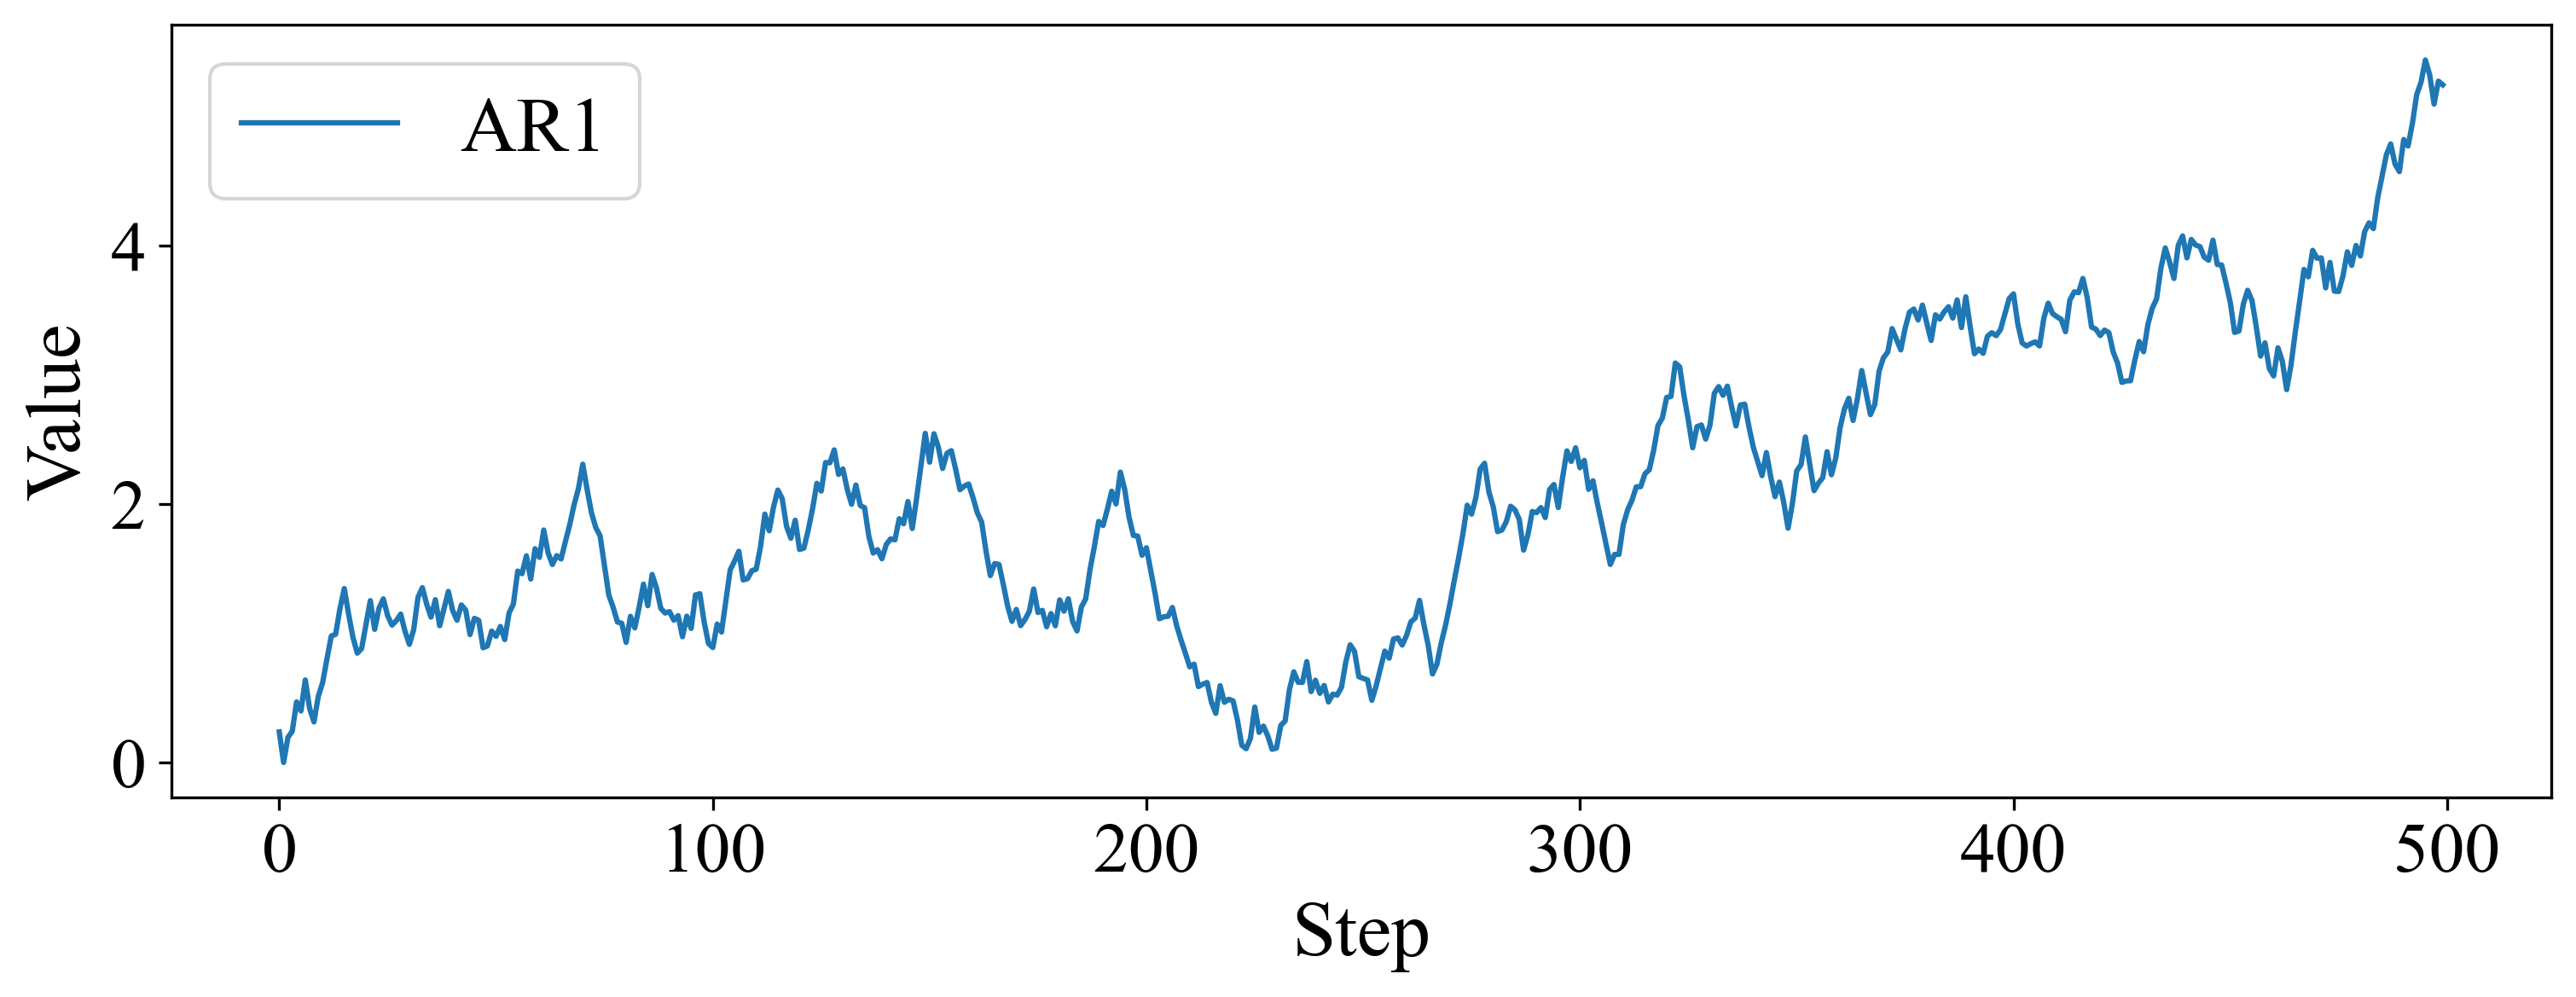
\includegraphics[width = 0.9\textwidth]{float/ch.app/ar1.png}
        \captionsetup{skip=2pt}
        \setlength{\belowcaptionskip}{-8pt}
        \caption{AR1合成数据\label{fig:app.ar1}}
    \end{figure}
    
\end{otherDatas}
% \phantomsection
% \input{body/chapter/univ.tex}

\end{appendix}

\end{document}
